% ===============================================================================
% $Id: R-2010-008 Higgs Manual.tex 2632 2011-09-28 17:06:29Z parjonilla $
% ===============================================================================
%
% Title: Higgs Manual
% Author:  C.Hernandez, A. Hernando, Paco Arjonilla and R.Sanz,
%
% Release: $Revision: 2632 $
% Author: $Author: parjonilla $
% Date:  $Date: 2011-09-28 19:06:29 +0200 (Wed, 28 Sep 2011) $
%
% Copyright (c) $Year$ ASLab
%
%=============================================================================== 

\documentclass{aslreport}

\usepackage{color}
\usepackage{url}
\usepackage[latin1]{inputenc}
\usepackage{graphicx} \graphicspath{{figures/}}

% Standard quote (text+reference)

\newcommand{\Quote}[2]{
\begin{quotation}
\noindent\textit{``#1''}\\
\cite{#2}
\end{quotation}
}

% Quote with additional information

\newcommand{\QuoteX}[3]{
\begin{quotation}
\noindent\textit{``#1''}\\
\cite[#3]{#2}
\end{quotation}
}

% Chapter introductory quote

\newcommand{\QuoteI}[3]{
\begin{quotation}
\noindent\textit{``#1''}\\
\cite[#3]{#2}
\end{quotation}
\begin{center}
$\clubsuit$\\[1cm]
\end{center}
}

% Standardised figure

\newcommand{\Figure}[4]{
\begin{figure}[!htb]\centering
\includegraphics[width=#2]{#1}
\emph{\caption{#3}\label{#4}}
\end{figure}
}


% Abreviatures

\newcommand{\xie}{\emph{i.e.}\ }
\newcommand{\xeg}{\emph{e.g.}\ }
\newcommand{\xcf}{\emph{cf.}\ }
\newcommand{\xetc}{\emph{etc.}\ }

\newcommand{\gcaterm}[1]{\textsf{#1}}

\hyphenation{
sour-ce
im-pas-ses
me-thod
en-vi-ron-ment
know-ledge
ge-ne-ral
be-ha-viours
con-di-tions
ex-pres-sing
a-dap-ta-tion
ar-chi-tec-tures
smal-ler}


\begin{document}


% Document Metadata ========================================================
\title{Higgs Manual}
\subtitle{A Platform for Autonomy Research}
\date{\today}
\reference{R-2010-008}
\docyear{2010}
\release{0.1}
\status{Draft}
\author{Carlos Hern\'andez, 
Adolfo Hernando, 
Ricardo Sanz and
Francisco Arjonilla}
\logo{ASys_Logo.pdf}
\URL{http://www.aslab.org/documents/controlled/ASLAB-R-2010-008.pdf}
\abstract{The target system selected for control is a Pioneer 2 ATX robot.}
\keywords{Higgs, cognitive architecture, perception, action, integrated control,
cognition, emotion, autonomy, autonomous systems} \acknowledgements{We acknowledge the support of the European Commission through
grant \emph{IST-027819-IP ICEA} of the IST-2004-2.4.8 Cognitive Systems domain
and of the Spanish Ministry of Science and Innovation through grant
\emph{TIN2008-02250-E-1}.}
% =====================================================================
\maketitle

\abstractpage

%=====================================================================
\chapter*{Revisions}

\newcommand{\Revision}[4]{\small #1 & #2 & \parbox{6cm}{\raggedright\rule{0mm}{5mm}#3\rule[-3mm]{0mm}{4mm}}& \parbox{2cm}{\rule{0mm}{5mm}#4\rule[-3mm]{0mm}{4mm}} \\
\hline}

\begin{table}[htdp]
\centering
\begin{tabular}{|c|c|l|l|}\hline\hline
%====================================================================
Release & Date & Content & Author \\ \hline\hline
%====================================================================
\Revision{0.1}{10/05/04}{Initial release.}{Sanz}\hline
%====================================================================
\Revision{0.2}{28/09/11}{User and developer manuals.}{Arjonilla}\hline
%====================================================================
\end{tabular}
\label{table:revisions}
\end{table}%

%=====================================================================

\tableofcontents

%===========================================================================
\chapter{Introduction}
\label{chapter:introduction}
%===========================================================================

\section{Document Purpose}

The ASys search for universal cognitive architectures generalises insights
gained in the study of animal brains, providing a model of cognition that effectively and
homogeneously integrates autonomic, emotional and cogniitive aspects.

This document describes the Higgs robot, part of the ASys Robot Control Testbed
(RCT) that has been selected as the target demonstration of the higher level cognitive dimensions into a physical
system. The SOUL cognitive architecture intends the exploitation of croscutting
design patterns to realise custom architectures targetted to specific uses.
While SOUL leverages detailed knowledge about mammal brains as of integration of
cognitive, emotional and autonomic aspects its main objective is to transcend the concrete brain
implementations improving engineering
capability for the construction of technical systems.

This implementation shall serve as vehicle for evaluating both the architecture
and the componental technologies generalising the components extracted from
biological models ---e.g. rat brain parts like the amygdala, the basal ganglia
or the hippocampus--- that are addressed in other research activities.

\section{Content}

This report describes the Higgs Robot Control Testbed.

\Figure{Higgs-01.png}{10cm}{The Higgs robot is the central objective of
development of the RCT, where the architecture for robust autonomy
is demonstrated.}{fig:higgs}

\section{Intended Audience}

This document is intended to provide a description of the concrete testbed for
all stakeholders involved in development and evaluation of the SOUL
architecture.

\section{Mandatory References}

The ASys project is the context for this work:

\begin{description}
\item [ASys Vision] includes a description of the long-term objectives of the research.
\item [OASys] contains the ontology under development for ASys.  
\end{description}

\section{Structure of the report}

This document purpose is to describe the implementation of a physical and
software asset. It consists of several chapters roughly organised in four
parts. Part 1 is dedicated to introductory materials that are useful to frame
the main content of the report. Part 2 describes the hardware. Part 3 is the
main content with the software and modelling description of the integrated architecture. 
Finally, Part 4 contains some appendices.

The content is as follows:

\begin{description}
  \item [Chapter 1] provides an overall description of the document
  and the context for this work. 
  \item [Chapter 2] contains the specification of the robot hardware.
  \item [Chapter 3] Describes the robot control software.
  \item [Chapter 4] contains an analysis of the mission.
\end{description}

\section{Format}

In the different chapters and section of this documents several systems or
devices are described, so as to make it perfectly clear, the description of
each one uses a tabular structure with the following formats: \\[2mm]
This is mandatory text\\ \texttt{this depends of each device}\\ \emph{this is a comment}.


\section{Acknowledgements}

This work has been partially supported by a European Commission grant to the
project ``Integrating Cognition, Emotion and Autonomy'' (ICEA IST-027819) and
by the ``Conscious Cognitive Control'' grant of the Ministry for Science and
Innovation.




%===========================================================================
\chapter{The Higgs Robot Control Testbed}
%===========================================================================
The Robot Control Testbed (RCT) is a collection of robot--based applications
under development in the research group ASLab. The robots include commenrcial
research platforms, simulated robotos and custom mobile robot
implementations. 

Higgs is a custom robot that is part of thr RTC developments. This is a mobile
robotic system which consists of a base platform and different interconnected
subsystems to cover a wide range of capabilities. The research aim is to
provide the mobile robot with the necessary cognitive capabilities and an
intelligent control system, as to perform complex tasks. 

This manual includes information concerning its software and
hardware description, specification, and use cases and additional information.
 The following sections summarise the key aspects of the testbed.

\section{Higgs Structural Description}

\subsection{Base Platform}
The base platform of Higgs is a mobile robot Pioneer 2--AT8 which has been
designed by ActivMedia Robotics (Fig. \ref{Higgs}). It is a robust platform which includes all the necessary elements to implement a control and navigating system, specially designed for outdoor applications.  Additional systems and elements can be attached to this platform. The base platform is given the ASLab name Higgs, as a reference to the Higgs' bosson.\\
 
\begin{figure}[htdp]
\begin{center}
 {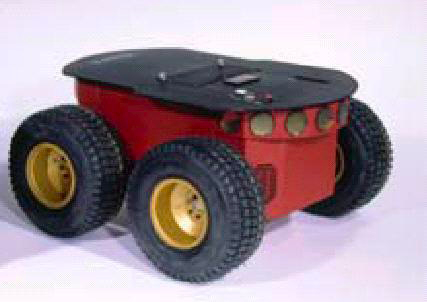
\includegraphics[width=0.75\textwidth]{Higgs.jpg}}
\end{center}
\caption{The Pioneer 2-AT8 platform used to implement the RCT Higgs robot.}
\label{Higgs}
\end{figure}


Higgs is a small size mobile robot, with a support structure made of aluminium. Its total weight is of 15 kg, being capable of carrying up to 40 kg. From a hardware viewpoint, the mobile robot consists of different elements: 

%AUG 2009 BE AWARE: each subsystem or element should have both an structural and a functional brief description!!
\begin{description}
\item Robot Panel: it is the superior platform of the robot, designed for a later assembly of new elements such as cameras or laser systems. 
\item Robot Body: it is a box--shaped element made of aluminium. It contains the batteries, the actuators, the electronic circuits and the rest of elements. It also allows to attach additional elements such as an onboard PC, a modem or additional sensors.
\item Control Panel: it is the access panel to the robot's microcontroller, placed in the robot panel. It consists of several control buttons, robot status leds (robot switch on, microcontroller status, battery charge) and a serial port RS--232 to be used as an input and output communication link with a external PC.
\item Sensors: the mobile robot is provided with two arrays of eight sensors each, which allow the detection and location of objects in the mobile robot environment. The arrays are placed at the front and at the rear part of the robot.
\item Actuators: the robots contains 4 Pittman motors GM9236E204. Each one includes an optical encoder to determine the robot's speed and position. 
\item Microcontroller: it is a Hitachi H8S microcontroller consisting of different elements (memories, serial ports, inputs, outputs, 8 bit bus) which carries out different operations such as trigger and register the sensors' signal, control the actuators, and some other low--level operations.
\item Bumpers: they are additional elements attached to the platform, 5 at the front and 5 at the rear.
\item Power: there are three batteries 12 VDC 7 Ah--h, located at the rear part of the robot. They provide 252 W--h, which assure several hours of autonomy movement to the robot. Their status can be checked in the corresponding led of the control panel.
\end{description}

% From HiggsManual. There is much more than the things written here
In addition to the hardware, the mobile robot has different software elements, either provided by the manufacturer or developed by ASLab team members. 
\begin{description}
\item AROS (ActivMedia Robotics Operating System): it is the operating system, consisting in server processes running on the Hitachi microcontroller in Higgs. It is a low--level software in charge of regulating the motors' speed, sonars' signal, encoders' signal and other low--level tasks. This software will also communicate the obtained information to other client software applications through the RS-232 serial interface.
\item ARIA: it is an applications--programming interface (API) based on C++ to control the robot. It acts as the client in the client--server topology. It allows to program high--level software applications, such as intelligent behaviour (obstacle avoidance, object recognition, wandering, exploration, etc). The robot control is based on direct commands, movement commands or abstract--level actions.
\item ASLab team software: there are a set of modules developed by the ASLab team members to extend or to add capabilities of Higgs. The modules developed are: communication \cite{Pareja2004}, synthetic emotions \cite{Conde2005}, SOAR integration \cite{Sanchez2005}, voice \cite{Panizo2005}, RT--CORBA control server \cite{Hernando2005}, RT--CORBA robot status register, Java based CORBA client, CORBA based remote operation \cite{Conejo2007}, and surface recognition \cite{Godoy2007}. 
\end{description}

%some of the last devices not included in Manual Higgs, so not much info!!
\subsection{Onboard Systems}

On the base platform, different devices have been attached to expand the original range of functionalities of the mobile robot (Fig. \ref{higgswithonboarddevices}).\\

\begin{figure}[htdp]
\begin{center}
 {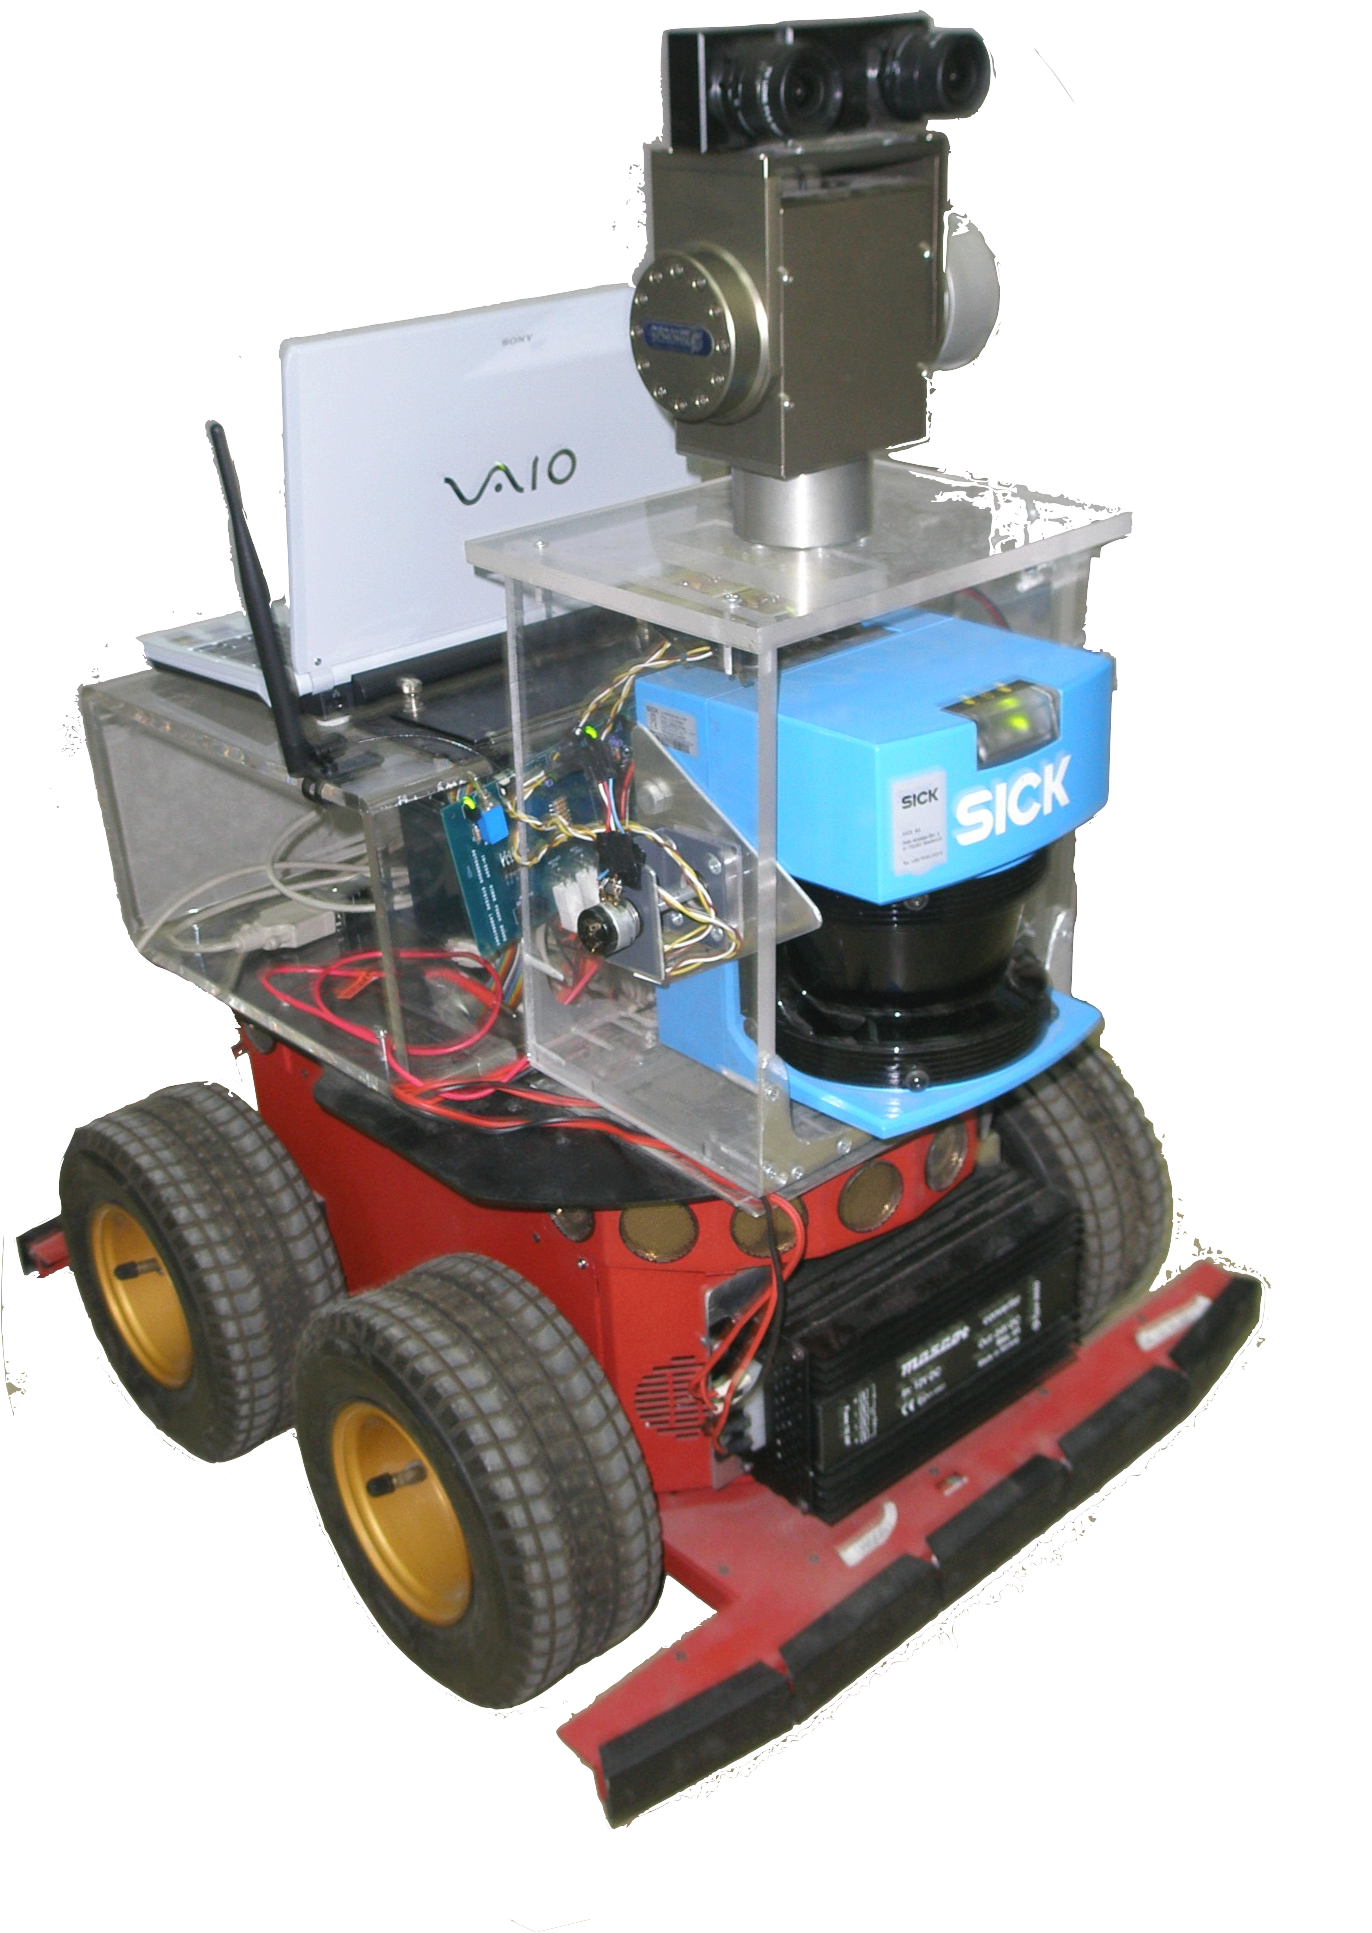
\includegraphics[width=0.65\textwidth]{higgs.png}}
\end{center}
\caption{Pioneer 2-AT8 (Higgs) with onboard systems}
\label{higgswithonboarddevices}
\end{figure}

\begin{itemize}
\item Onboard Computer:  it is a computer attached to the base platform whose mission is to facilitate the communication with the microcontroller, the control of the robot, the execution of complex navigation operations, and additional communication operations. Taking into consideration several requirements and operational constraints defined in \cite{ManualHiggs}, a GENE--6330 was chosen. Related to software, the onboard computer uses Linux as operating system, as well as having a real--time software RTAI and RT--CORBA server.
\item Laser: it is a laser scanner for mobile robotics applications, placed at the front part of the robot panel.
\item Wrist: it is a 2 DOF high precision and torque actuator for orientation of the camera. It is attached to the laser.
\item Camera: it is a stereo camera that will be used as the robot's vision system, attached to the wrist.
\item Radio: it is a radio system for DGPS.
\item Laptop: it is a lightweight high functional laptop.
\item GPS: it is a high performance GPS system.
\end{itemize}

\subsection{Supporting Systems} 
Along with the base platform and the onboard systems, Higgs includes some
additional supporting systems to complete its functioning.

\begin{enumerate}
\item Wireless Network: it is an additional subsystem included in the testbed to allow the communication with the wireless local network in the ASLab laboratory. It consists of a wireless card (placed in the onboard computer), an antenna necessary as the wireless card is placed inside the aluminium robot body (attached to the robot panel), and an access point (connected to the laboratory LAN).
\item Remote Control: it is a portable device to remote control the robot.
\item Server
\item User Terminal
\end{enumerate}

\section{Robot Functional Description}

The functional description of the Higgs robot Testbed has been made
through the specification of use cases and requirements (see Chapter
\ref{chapter:asyshiggs}). \emph{FunctionalRequirement} has been defined in the
ontology as a requirement that specifies an operation or behaviour a system must perform.\\

For the RCT, the functional requirements considered can be classified into primary  and secondary ones. A primary functional requirement refers to a main capability to be fulfilled by the system. In the case of the RCT, two primary functional requirements have been considered: navigation, and survival. \\

A secondary functional requirement refers to an additional capability desired in the system. For the RCT, these secondary functional requirements are: to explore the environment, to avoid an obstacle while moving or exploring, reactive movement, the identification of an object in the environment, and search. Some additional functional requirements expand or detail the former ones, such as autonomous navigation as an extended case of the navigation one.\\




%===========================================================================
\chapter{Physical System Specification}
%===========================================================================

The RCT testbed is a mobile robotic system intended as platform to test the
technology developed in ICEA. The RCT platform is a pioneer mobile robot for
research that is specially designed for outdoors applications. The aim of the
RCT testbed is to purvey the system with the neccessary cognitive abilities so
as to fulfil complex task. This abstract aim is grounded in the specification of a high level mission and the evaluation of the OM consciousness architecture as to enhenace mission level robustness.

In this document the overall situation of the RCT platform of the ICEA Project
is presented. The purpose of the document is double:

\begin{itemize}
  \item Report the current state of the platform.
  \item Provide a short description of the platform.
\end{itemize}

The specification section is presented in the form of tables of specifications to capture the
main characteristics of the different devices that compose the RCT platform. For
much more detailed information on the RCT platform please refer to Higg's Manual ?poner enlace?






%------------------------------------------------------------------------------

	
	

\section{Base Platform: Pioneer 2-AT8}

%------------------------------------------------------------------------------
\begin{table}
\centering
\hspace{-4cm}
\begin{tabular}{|l|l|}
\hline

\textbf{RCT Identifier}: & RCT-Higgs \\
\hline

\textbf{RCT Name}: & Higgs \\
\hline

\textbf{Description}: & mobile robot for outdoors use \\
\hline

\textbf{Functionality role}: & Robot base \\
\hline

\textbf{Model}: & Pioneer 2AT-8 \\
\hline

\textbf{State}: & fully operative \\
\hline

\textbf{Serial number}: & AT8CDBB1722 \\
\hline

\textbf{Purchase date}: & 200302 \\
\hline

\textbf{Physical Characteristics}: & 
\parbox{8cm}{
	\begin{tabular}{l l}
    	\multicolumn{2}{l}{Alluminium body}\\
		\textbf{Dimensions} & 50x49x24 cm\\	
		\textbf{Weight} & 15 kg\footnote{one battery onboard}\\	
		\textbf{Payload} & 40 kg\\		
	\end{tabular}
}
 \\
\hline

\textbf{Physical links}: & 
\parbox{8cm}{
	\begin{tabular}{l l}
	\textbf{} & \\
	
	\textbf{} & \\
	
	\textbf{} & \\
		
	\end{tabular}
}

 \\
\hline

\textbf{Informational links}: & 
\parbox{8cm}{
	\begin{tabular}{l l}
	\textbf{In} & 5 analog\\
	
	\textbf{Out} & 2 analog\\
	
	\textbf{In\&Out} & 3 RS-232 ports, 8 bits bus\\
		
	\end{tabular}
}

 \\
\hline

\textbf{Power}: &  3 batteries 12VDC 7A-h (252W-h) \\
\hline

\textbf{Features}: & 

\parbox{10cm}{
	\begin{tabular}{l p{6.5cm}}
	\textbf{Microcontroller} & Hitachi H8S\\
	\textbf{Actuators:}	& \textbf{Skid steering:} \small{4 pittman motors
	GM9236E204}\\
	\textbf{Sensors:}	& \textbf{Sonar:} \small{2 arrays (front\&rear)  each of 8
	sensors, 20�}  \\
	& \textbf{Encoders:} \small{1 per wheel-- 34,000 conts/rev}\\
	& \textbf{Bumpers:} \small{5 front and 5 rear}\\
	\end{tabular}
	\\
	}
	\\

\textbf{Tech. doc.}: & \\
\hline

\end{tabular}
\end{table}
%-------------------------------------------------------------------------------


\section{Onboard Systems}

\subsection{Gene-6330}

%------------------------------------------------------------------------------
\begin{table}[ht!]
\centering
\hspace{-4cm}
\begin{tabular}{|l|l|}
\hline

\textbf{RCT Identifier}: &  RCT-Gene\\
\hline

\textbf{RCT Name}: &  placa Gene\\
\hline

\textbf{Description}: &  This is the onboard computer\\
\hline

\textbf{Functionality role}: & On board computer \\
\hline

\textbf{Model}: &  GENE-6330\\
\hline

\textbf{State}: &  Obsolete and retired\\
\hline

\textbf{Serial number}: &  \\
\hline

\textbf{Purchase date}: &  \\
\hline

\textbf{Physical Characteristics}: & 
\parbox{8cm}{
	\begin{tabular}{l l}
    	\textbf{Dimensions} & 146x101.6x26mm mm\\	
		\textbf{Weight} & 0.4 kg
	\end{tabular}
}\\
\hline

\textbf{Physical links}: & 
\parbox{8cm}{
	\begin{tabular}{l l}
		\textbf{} & attached inside Higgs\\			
	\end{tabular}
}\\
\hline

\textbf{Informational links}: &
\parbox{10cm}{
	\begin{tabular}{l p{7.5cm}}
		1 ethernet (RJ-45)	&	not used \\
		1 configurable port	RS-232/422/485 & not used\\
		1 port RS-232 (need to put a conector) & not used\\
		Wifi (purveyed by Compact PCMCIA) & main external interface\\
	\end{tabular}
}
\\
\hline

\textbf{Power}: &  typical 0.7W / Max 6.4W (+5V and +12V AT) from higgs
batteries\\
\hline

\textbf{Features}: & 
\parbox{10cm}{
	\begin{tabular}{l p{6cm}}
		\textbf{Microprocessor} & Transmeta Crusoe TM5400, 600MHz\\
		\textbf{Memory} & 64MB SDRAM + 256MB SDRAM\\
		\textbf{Flash Memory} & CompactFlash I type 4GB\\
		\textbf{Wifi} & purveyed by a Compaq WL110 PCMCIA + antenna\\
	\end{tabular}
}\\
\hline

\textbf{Tech. doc.}: & \\
\hline

\end{tabular}
\end{table}
%-------------------------------------------------------------------------------







\newpage
\subsection{Laptop}
%------------------------------------------------------------------------------
\begin{table}[ht!]
\centering
\hspace{-4cm}
\begin{tabular}{|l|l|}
\hline

\textbf{RCT Identifier}: &  RCT-laptop\\
\hline

\textbf{RCT Name}: &  vaio\\
\hline

\textbf{Description}: &  a lightweith high functional laptop\\
\hline

\textbf{Functionality role}: & On board computer \\
\hline

\textbf{Model}: & Sony Vaio TX2HP \\
\hline

\textbf{State}: &  Fully operative \\
\hline

\textbf{Serial number}: &  \\
\hline


\textbf{Purchase date}: &  \\
\hline

\textbf{Physical Characteristics}: & 
\parbox{8cm}{
	\begin{tabular}{l l}
		\textbf{Dimensions} & \\	
		\textbf{Weight} & \\	
	\end{tabular}
}\\
\hline

\textbf{Physical links}: & The Vaio is attached to the back part of Higgs' top \\
\hline

\textbf{Informational links}: & 
\parbox{8cm}{
	\begin{tabular}{l p{8cm}}
		\textbf{In\&Out} &  2 USB 2.0, wifi IEEE 802.11b/g, 1 ethernet, Bluetooth
		2.0\\
	\end{tabular}
}\\
\hline

\textbf{Power}: &  from its internal battery (7.5 hour)\\
\hline

\textbf{Features}: & 
\parbox{10cm}{
	\begin{tabular}{l p{6.5cm}}
		\textbf{Processor} & Intel Pentium M 1.1GHz\\
		\textbf{Memory} & 510 MB DDR2 SDRAM\\
		\textbf{OS} & Windows XP and Fedora ??\\
		\textbf{Hard drive} & 80 GB -4200 rpm\\
		\textbf{Display} & 11.1'' LCD\\
		\textbf{DVD+RW} & \\
	\end{tabular}
}\\
\hline

\textbf{Tech. doc.}: & \\
\hline

\end{tabular}
\end{table}
%-------------------------------------------------------------------------------

\newpage
\subsection{Arduino}
%-------------------------------------------------------------------------------
\begin{table}[ht!]
\centering
\hspace{-4cm}
\begin{tabular}{|l|p{10cm}|} 
\hline

\textbf{RCT Identifier}: &  RCT-arduino\\
\hline

\textbf{RCT Name}: &  arduino\\
\hline

\textbf{Description}: &  a simple board to conect some simple devices\\
\hline

\textbf{Functionality role}: & I/O board \\
\hline

\textbf{Model}: &  \\
\hline

\textbf{State}: &  Fully integrated \\
\hline

\textbf{Serial number}: &  \\
\hline

\textbf{Purchase date}: &  2007\\
\hline

\textbf{Physical Characteristics}: &
\parbox{8cm}{
	\begin{tabular}{l l}
		\textbf{Dimensions} & 175x55x50 \\
	\end{tabular}
}\\
\hline

\textbf{Physical links}: & Attached to the left side of the laser support\\
\hline

\textbf{Informational links}: &
\parbox{8cm}{
	\begin{tabular}{l l}
		USB & connected to laptop\\
		3-wire & connected to various sensors\\
	\end{tabular}
}\\
\hline

\textbf{Power}: & 6-12 VDC \\
\hline

\textbf{Features}: &
\parbox{10cm}{
	\begin{tabular}{l p{6.5cm}}
		\textbf{Sensors} & 2 accelerometers, 1 compass, 2 current and voltage sensors,
				1 servo, 1 potentiometer, 2 switches.
	\end{tabular}
}\\
\hline

\textbf{Tech. doc.}: & \\
\hline

\end{tabular}
\end{table}
%-------------------------------------------------------------------------------




\subsection{Laser}

%------------------------------------------------------------------------------
\begin{table}[ht!]
\centering
\hspace{-4cm}
\begin{tabular}{|l|l|}
\hline

\textbf{RCT Identifier}: &  RCT-Laser\\
\hline

\textbf{RCT Name}: &  Laser\\
\hline

\textbf{Description}: &  laser scanner for mobile robotics applications, SLAM,
navigation, etc\\
\hline

\textbf{Functionality role}: & Scan device \\
\hline

\textbf{Model}: &  Sick LMS-200\\
\hline

\textbf{State}: &  Integrated\\
\hline

\textbf{Serial number}: &  \\
\hline

\textbf{Purchase date}: &  \\
\hline

\textbf{Physical Characteristics}: & 
\parbox{8cm}{
	\begin{tabular}{l l}
		\textbf{Dimensions} & 155x156x265mm\\	
		\textbf{Weight} & 4.5kg\footnote{without the support}\\	
	\end{tabular}
}\\
\hline

\textbf{Physical links}:
& The laser support is screwed to the front part of Higgs' top. \\
& Includes a mechanism for tilting the laser by means of a servo.\\
& The RCT-Wrist is screwed to the top of the laser support
\\
\hline

\textbf{Informational links}: & 
\parbox{8cm}{
	\begin{tabular}{l l}
		RS-232/\textbf{422} & connected to vaio through USB/RS-232 converter\\	
	\end{tabular}
}\\
\hline

\textbf{Power}: & 24VDC 40 W\\
\hline

\textbf{Features}: & 
\parbox{10cm}{
\begin{tabular}{l p{5cm}}
  \textbf{Scanning angle} & 180� \\
  \textbf{Res\/typ. meas. accuracy} & 10mm$/\pm$35mm  \\
  \textbf{Accesories} & Metacrilate support $\pm$45� tilt with a Futaba servo \\	
\end{tabular}
} \\
\hline

\textbf{Tech. doc.}: & \\
\hline

\end{tabular}
\end{table}
%-------------------------------------------------------------------------------
\newpage

\subsection{Camera}
%------------------------------------------------------------------------------
\begin{table}[ht!]
\centering
\hspace{-4cm}
\begin{tabular}{|l|l|}
\hline

\textbf{RCT Identifier}: &  RCT-Camera\\
\hline

\textbf{RCT Name}: &  Camara\\
\hline

\textbf{Description}: &  Stereo camera for Higgs' vision system\\
\hline

\textbf{Functionality role}: & Camera \\
\hline

\textbf{Model}: &  Videre STH-MDCS2-C\\
\hline

\textbf{State}: &  available, already controlled independently but not
integrated\\
\hline

\textbf{Serial number}: &  \\
\hline

\textbf{Purchase date}: &  \\
\hline

\textbf{Physical Characteristics}: & 
\parbox{8cm}{
	\begin{tabular}{l l}
		\textbf{Dimensions} & 44x132x73 mm\\	
		\textbf{Weight} & 330 g\\	
	\end{tabular}
}\\
\hline

\textbf{Physical links}: & 
		Screwed to RCT-Wrist\\
\hline

\textbf{Informational links}: & 
\parbox{8cm}{
	\begin{tabular}{l l}
		\textbf{In\&Out} & ieee 1394 (firewire)\\	
	\end{tabular}
}\\
\hline

\textbf{Power}: &  $<$ 1W - 12 VDC\\
\hline

\textbf{Features}: & 
\parbox{10cm}{
	\begin{tabular}{l p{6.5cm}}
		\textbf{Accesories} & RCT-Wrist\\	
	\end{tabular}
}\\
\hline

\textbf{Tech. doc.}: & \\
\hline

\end{tabular}
\end{table}
%-------------------------------------------------------------------------------
\newpage
\subsection{Wrist}
%------------------------------------------------------------------------------
\begin{table}[ht!]
\centering
\hspace{-4cm}
\begin{tabular}{|l|p{9cm}|}
\hline

\textbf{RCT Identifier}: &  RCT-Wrist\\
\hline

\textbf{RCT Name}: &  Wrist \\
\hline

\textbf{Description}: &  2 DOF high precision and torque actuator for
orientation (pan\&tilt) of the RCT-camera\\
\hline

\textbf{Functionality role}: & Wrist \\
\hline

\textbf{Model}: &  SCHUNK PW-070\\
\hline

\textbf{State}: &  Fully integrated \\
\hline

\textbf{Serial number}: &  B3844 \& B3844\\
\hline

\textbf{Purchase date}: &  \\
\hline

\textbf{Physical Characteristics}: &
\parbox{8cm}{
	\begin{tabular}{l l}
    	\multicolumn{2}{l}{}\\
		\textbf{Dimensions} & 165x70x160 mm aprox\\
		\textbf{Weight} & 1.8 kg\\
	\end{tabular}
}\\
\hline

\textbf{Physical links}: &
\parbox{8cm}{
	\begin{tabular}{l l}
		\textbf{axis2 appendix} &  attached to laser support\\
		\textbf{axis1 appendix} &  camera is attached here\\
	\end{tabular}
}\\
\hline

\textbf{Informational links}: &
\parbox{8cm}{
	\begin{tabular}{l l}
		\textbf{In\&Out} & RS-232\\
	\end{tabular}
}\\
\hline

\textbf{Power}: & 24 VDC, nomical power current 4 A per axis \\
\hline

\textbf{Features}: &
\parbox{10cm}{
	\begin{tabular}{l p{6.5cm}}
		\textbf{Sensors} & 1 encoder per axis\\
		\textbf{Nominal torque} & 12 Nm axis1, 2 Nm axis2 \\
		\textbf{Algle of rotation} & 120� axis1, 360� axis2 \\
		\textbf{Resolution} & 5'' axis, 6'' axis2
	\end{tabular} 
}\\
\hline

\textbf{Tech. doc.}: & \\
\hline

\end{tabular}
\end{table}
%-------------------------------------------------------------------------------


\newpage
\subsection{GPS}
%------------------------------------------------------------------------------
\begin{table}[ht!]
\centering
\hspace{-4cm}
\begin{tabular}{|l|l|}
\hline

\textbf{RCT Identifier}: &  RCT-GPS\\
\hline

\textbf{RCT Name}: &  GPS\\
\hline

\textbf{Description}: &  high performance GPS system\\
\hline

\textbf{Functionality role}: & GPSd \\
\hline

\textbf{Model}: &  OEMV-2-RT2\\
\hline

\textbf{State}: &  ready to install\\
\hline

\textbf{Serial number}: &  \\
\hline

\textbf{Purchase date}: &  2007\\
\hline

\textbf{Physical Characteristics}: &
\parbox{8cm}{
	\begin{tabular}{l l}
		\textbf{Dimensions} & 60x100x13 mm\\
		\textbf{Weight} & 56 g\\
	\end{tabular}
}\\
\hline

\textbf{Physical links}: &
\parbox{8cm}{
	\begin{tabular}{l l}
		\textbf{} & \\
	\end{tabular}
}\\
\hline

\textbf{Informational links}: &
\parbox{8cm}{
	\begin{tabular}{l l}
		\textbf{1 USB} & connected to laptop\\
		1 RS-232/422\\
		1 CAN bus & not used\\ 
	\end{tabular}
}\\
\hline

\textbf{Power}: &  1.6W typ. \/ 12 VDC\\
\hline

\textbf{Features}: &
\parbox{10cm}{
	\begin{tabular}{l p{6.5cm}}
		\textbf{Accuracy} & \\
		\textbf{Accesories} & RCT-radio \\
							& Antenna	\\
	\end{tabular}
}\\
\hline

\textbf{Tech. doc.}: & \\
\hline

\end{tabular}
\end{table}
%-------------------------------------------------------------------------------

\subsection{Power Board}
%------------------------------------------------------------------------------
\begin{table}[ht!]
\centering
\hspace{-4cm}
\begin{tabular}{|l|l|}
\hline

\textbf{RCT Identifier}: &  PowerBoard\\
\hline

\textbf{RCT Name}: &  Power Board\\
\hline

\textbf{Description}: &  A simple board for controlling power to other devices\\
\hline

\textbf{Functionality role}: & Power board \\
\hline

\textbf{State}: &  Fully operative\\
\hline

\textbf{Serial number}: &  \\
\hline

\textbf{Manufacturing date}: &  October 2009\\
\hline

\textbf{Physical Characteristics}: &
\parbox{8cm}{
	\begin{tabular}{l l}
		\textbf{Dimensions} & 260x86x16 mm\\
	\end{tabular}
}\\
\hline

\textbf{Physical links}: & Attached to the front of the Vaio support \\
\hline

\textbf{Informational links}: &
\parbox{8cm}{
	\begin{tabular}{l l}
		\textbf{Ribbon cable} & attached to arduino board\\
		\textbf{Input 12V} & connected to Inst. batteries\\
		\textbf{12V-24V} & to connect a 12V to 24V converter\\
		\textbf{Input 24V} & connected to 12V to 24V converter\\
		\textbf{6x12V} & Power for 12V devices\\
		\textbf{3x24V} & Power for Wrist, Laser and 1 free slot\\
		\textbf{Power Jack} & Battery charger\\
	\end{tabular}
}\\
\hline

\textbf{Power}: &  negligible, 12V to 24V \\
\hline


\textbf{Tech. doc.}: & \\
\hline

\end{tabular}
\end{table}
%-------------------------------------------------------------------------------

\newpage
\subsection{Radio}
%-------------------------------------------------------------------------------
\begin{table}[ht!]
\centering
\hspace{-4cm}
\begin{tabular}{|l|p{10cm}|} 
\hline

\textbf{RCT Identifier}: &  RCT-radio\\
\hline

\textbf{RCT Name}: &  radio\\
\hline

\textbf{Description}: &  a radio system for DGPS (GPS + difference with a
known base = more precisssion)\\
\hline

\textbf{Functionality role}: & GPSd radio \\
\hline

\textbf{Model}: &  Pacific Crest PDLRVR\\
\hline

\textbf{State}: &  not installed\\
\hline

\textbf{Serial number}: &  \\
\hline

\textbf{Purchase date}: &  2007\\
\hline

\textbf{Physical Characteristics}: &
\parbox{8cm}{
	\begin{tabular}{l l}
		\textbf{Dimensions} & 21.0 cm L x 6.1 cm diameter\\
	\end{tabular}
}\\
\hline

\textbf{Physical links}: &
\parbox{8cm}{
	\begin{tabular}{l l}
		\textbf{} & \\
	\end{tabular}
}\\
\hline

\textbf{Informational links}: &
\parbox{8cm}{
	\begin{tabular}{l l}
		\textbf{} & \\
	\end{tabular}
}\\
\hline

\textbf{Power}: &  0.3W 9-16 VDC (from its own external battery)\\
\hline

\textbf{Features}: &
\parbox{10cm}{
	\begin{tabular}{l p{6.5cm}}
		\textbf{} & \\
		\textbf{Weight} & 0.34 kg\\
		\textbf{Accessories} & Antenna \\
							 & Battery \\
	\end{tabular}
}\\
\hline

\end{tabular}
\end{table}
%-------------------------------------------------------------------------------

\section{Supporting Systems}

\subsection{PSP Remote Control}
%------------------------------------------------------------------------------
\begin{table}[ht!]
\centering
\hspace{-4cm}
\begin{tabular}{|l|p{10cm}|}
\hline

\textbf{RCT Identifier}: &  RCT-PSP\\
\hline

\textbf{RCT Name}: &  psp\\
\hline

\textbf{Description}: &  a portable device with screen and controls to 
control remotely the RCT platform\\
\hline

\textbf{Functionality role}: & Remote controller \\
\hline

\textbf{Model}: & Sony PSP-1004 \\
\hline

\textbf{State}: &  available, not integrated\\
\hline

\textbf{Serial number}: &  \\
\hline

\textbf{Purchase date}: &  \\
\hline

\textbf{Physical Characteristics}: & 
\parbox{8cm}{
	\begin{tabular}{l l}
		\textbf{Dimensions} & 170x23x74 mm\\	
		\textbf{Weight} & 280 gr\\	
	\end{tabular}
}\\
\hline

\textbf{Physical links}: & none (it's portable) \\
\hline

\textbf{Informational links}: & 
\parbox{8cm}{
	\begin{tabular}{l l}
		\textbf{In\&Out} wifi (IEEE 802.11b), USB, infrared port\\	
	\end{tabular}
}\\
\hline

\textbf{Power}: &  from its internal batteries\\
\hline

\textbf{Features}: & 
\parbox{10cm}{
	\begin{tabular}{l p{6.5cm}}
    	\textbf{Screen} & LCD 4.3'' (16:9) \\
		\textbf{Wifi Security} & WEP, WPA (both AES \& TKIP)\\
		\textbf{Video Compression} & H.264/MPEG-4 AVC \\
	\end{tabular}
}\\
\hline

\end{tabular}
\end{table}
%-------------------------------------------------------------------------------


\newpage
\subsection{Remote Server}
% el servidor de nombres etc

\subsection{Wireless Network}

%------------------------------------------------------------------------------
\begin{table}[ht!]
\centering
\hspace{-4cm}
\begin{tabular}{|l|p{10cm}|}
\hline

\textbf{RCT Identifier}: &  aslab\_wireless \\
\hline

\textbf{RCT Name}: &  aslab\_wireless \\
\hline

\textbf{Description}: &  ASLab's wifi network at DISAM and its surroundings\\
\hline

\textbf{Functionality role}: & Wi-fi connection \\
\hline

\textbf{Access point}: & Linksys WAP54G \\
\hline

\textbf{State}: &  fully operative \\
\hline

\textbf{Serial number}: &  \\
\hline

\textbf{Purchase date}: &  \\
\hline


\textbf{Situation}: & the access point is currently situated in the library \\
\hline

\textbf{Encryption}: & None \\
\hline

\textbf{Features}: & \\
\hline

\textbf{Other}: & config: usr= ; psswd= \\
\hline

\end{tabular}
\end{table}




%===========================================================================
\chapter{User Manual}
%===========================================================================
\section{Functionality description}
\label{sec:usermanual_func}
The Robotic Control Testbed is a Mobile Robot built from a commercial robot base with added funcionality.
The robot base consists of a four wheel vehicle with position and speed control embedded, integrated power and control
electronics and 16 ultrasonic sensors that give readings on the distance to close obstacles. Additionally front and
rear bumpers have been installed for safeguarding the robot while operating it
in very constrained areas and for manual stopping.

The Laser range reader can measure distances from 8mm up to 80m, depending on configuration. Typically it will function
with a resolution of 1mm and a range of 8mm to 8m. It is the main sensor along with the odometer readings in SLAM
navigation. It can be rotated with the servo to make three dimensional maps. The mechanism operates in open loop
mode, which gives a low precision angular rotation, given the mechanical hystheresys and the thermal and age deviations
of set.

Next to the laser the I/O board, or data acquisition board, is a general purpose input output board that connects to a compass, a two axis accelerometer,
the servo that controls the laser's tilt movement, and two current and voltage sensors one for monitoring the consumption of the robot base and the other for the power board and related devices. These sensors and actuators are controlled through the I/O board module.

For outdoor applications there is a global absolute position sensor which consists of a GPS antenna,
Radio receiver and battery for receiving differential corrections from a base station and a GPS receiver that
processes the data and converts it to an easier format readable by the onboard computer.

Vision applications can make use of the binocular camera, that in combination with the wrist, which gives pan and
tilt movement to the camera with respect to the robot base and is located on top of the laser, can direct the
focus of the attention in almost any direction. The wrist is internally controlled in position, speed and acceleration,
which gives precise and accurate motion control to the camera.

The onboard computer runs a full capable operating system and is the communications hub for controlling remotely
all the devices on the robot. Software controlling the devices may be installed onboard or in a remote computer.

\subsection{Visual identification of devices}


\begin{figure}[ht]
\centering
 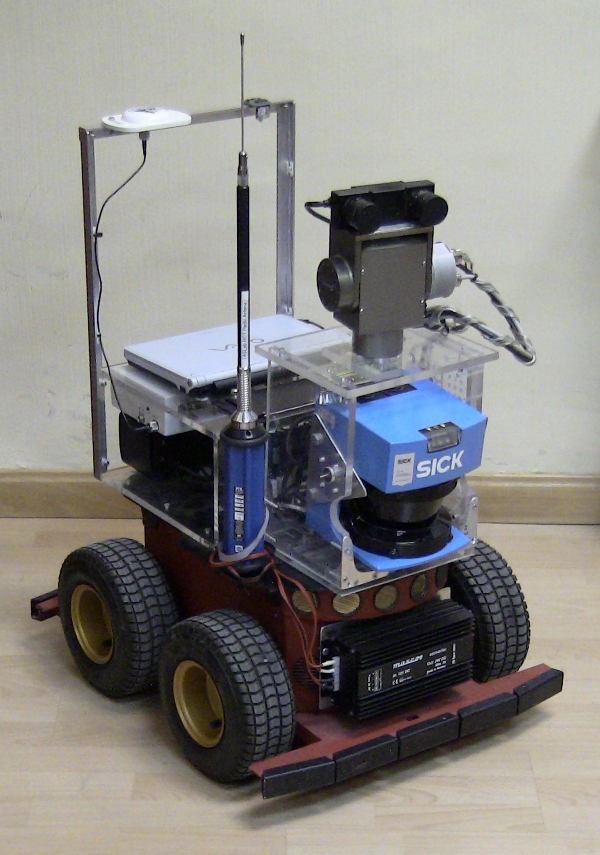
\includegraphics[width=0.4\textwidth]{figures/device_photos/higgs.jpg}
\caption{General view of Higgs.}
\end{figure}

\begin{figure}[ht]
\centering
 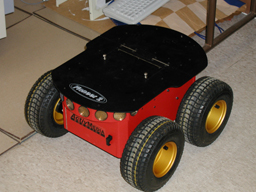
\includegraphics[width=0.4\textwidth]{figures/device_photos/p2at.jpg}
\caption{Robotic base Pioneer 2AT.}
\end{figure}

\begin{figure}[ht]
\centering
 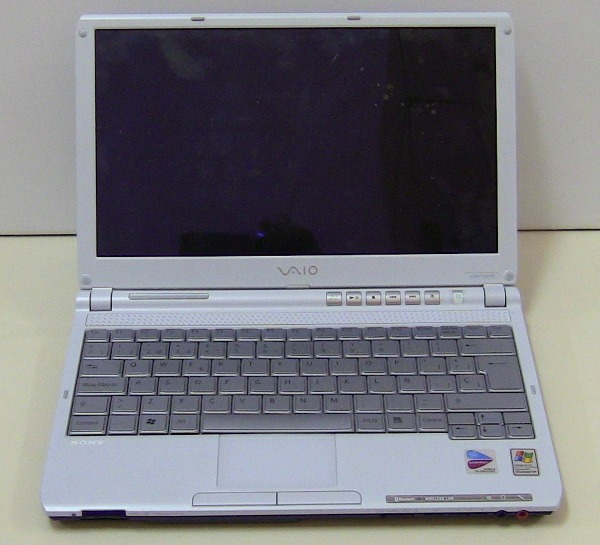
\includegraphics[width=0.3\textwidth]{figures/device_photos/vaio.jpg}
\caption{On board computer: VAIO laptop.}
\end{figure}

\begin{figure}[ht]
\centering
 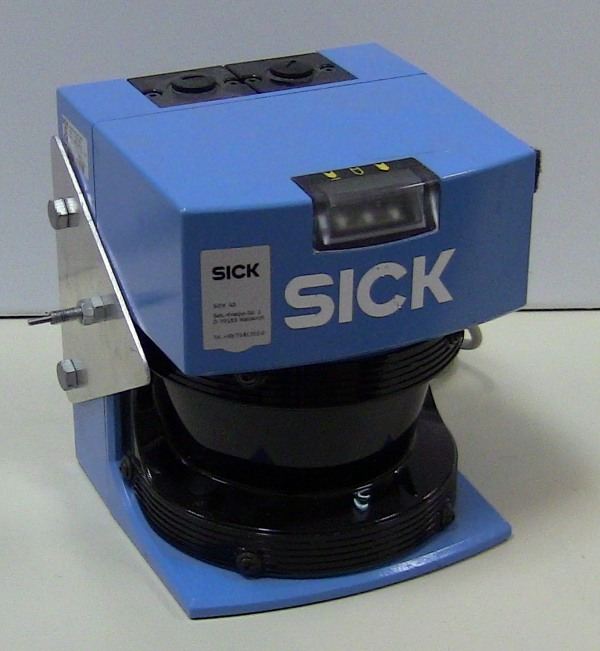
\includegraphics[width=0.3\textwidth]{figures/device_photos/laser.jpg}
\caption{Laser sensor.}
\end{figure}

\begin{figure}[ht]
\centering
 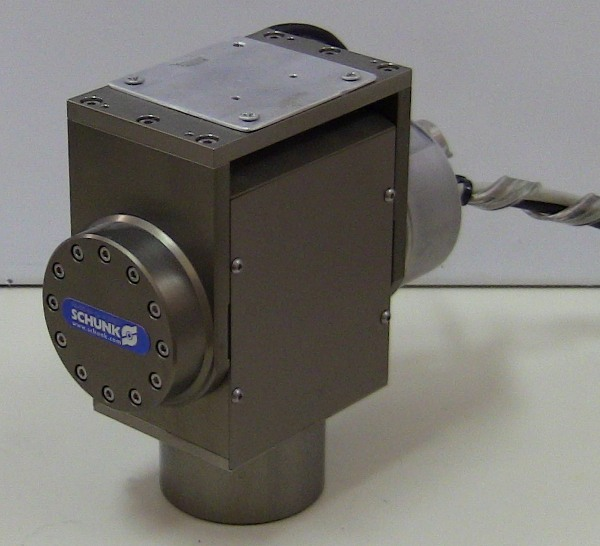
\includegraphics[width=0.4\textwidth]{figures/device_photos/wrist.jpg}
\caption{Wrist.}
\end{figure}

\begin{figure}[ht]
\centering
 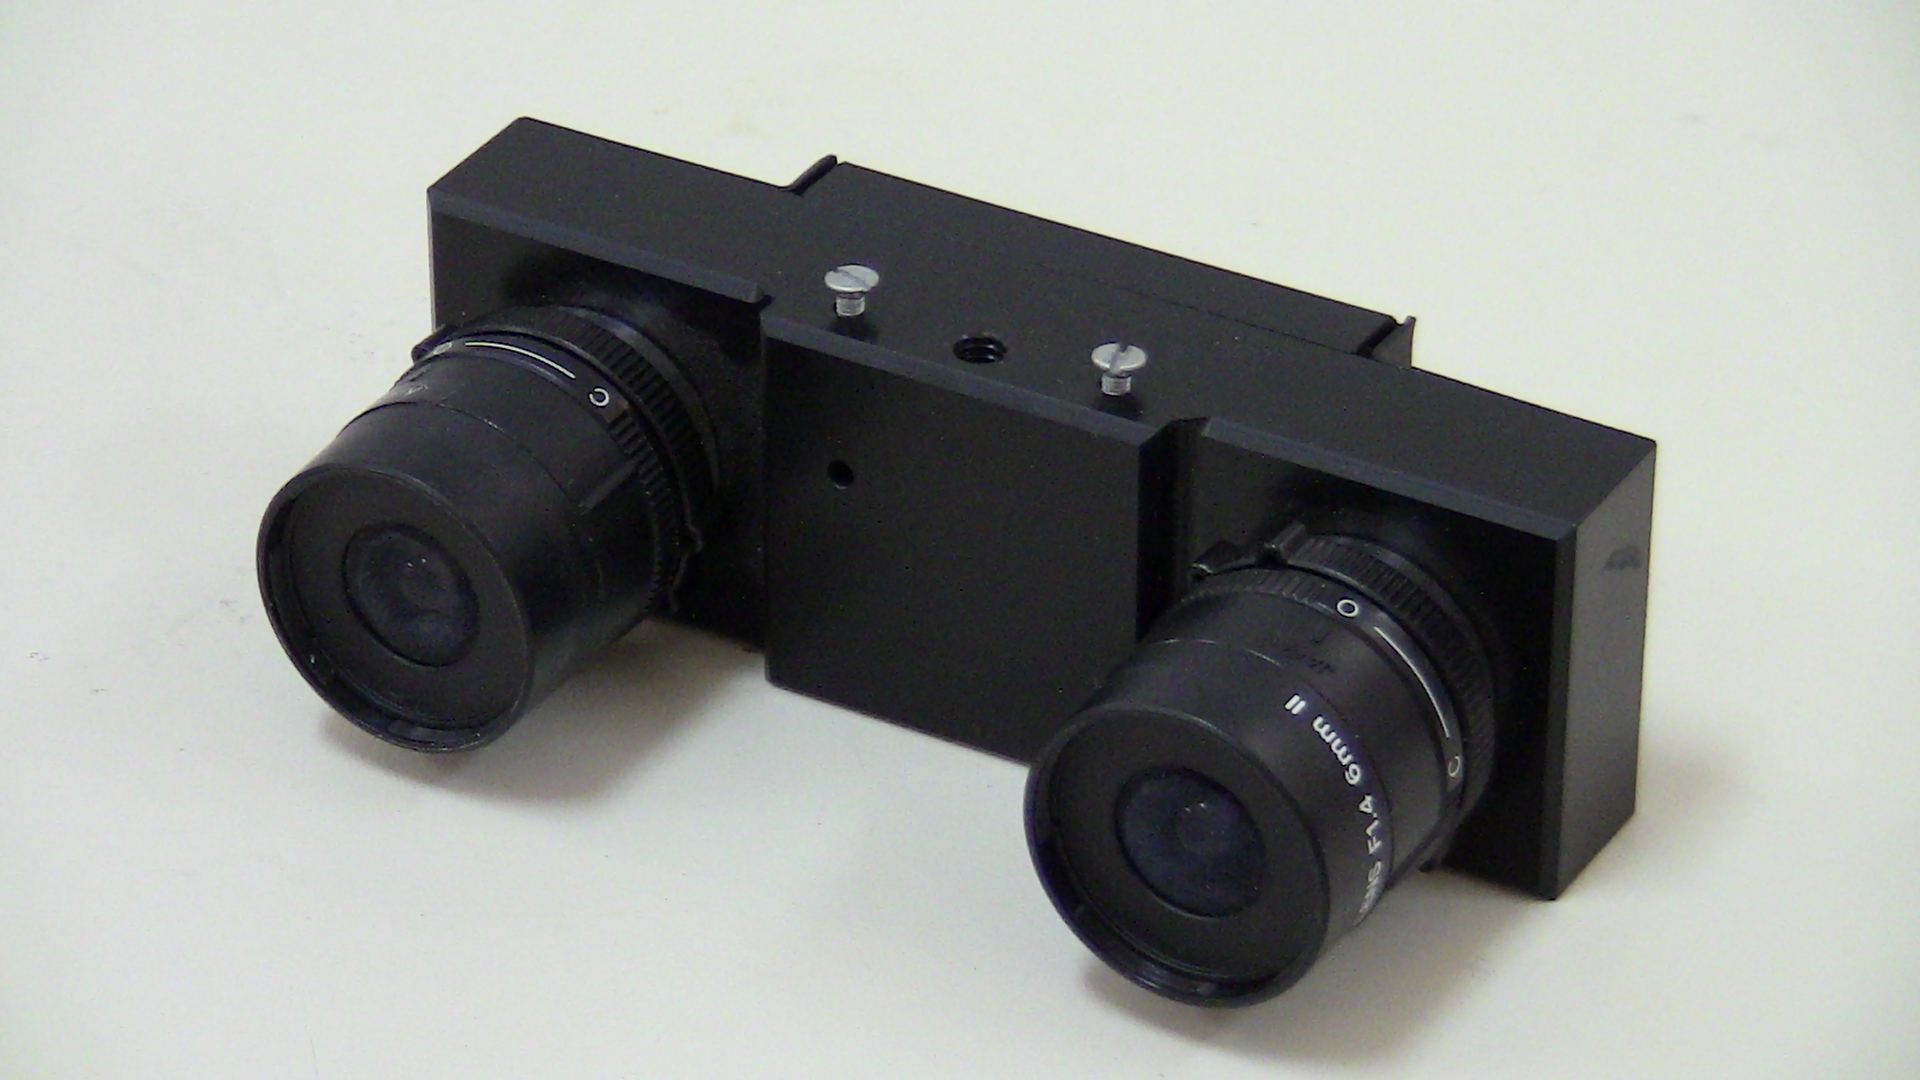
\includegraphics[width=0.4\textwidth]{figures/device_photos/camera.jpg}
\caption{Camera.}
\end{figure}

\begin{figure}[ht]
\centering
 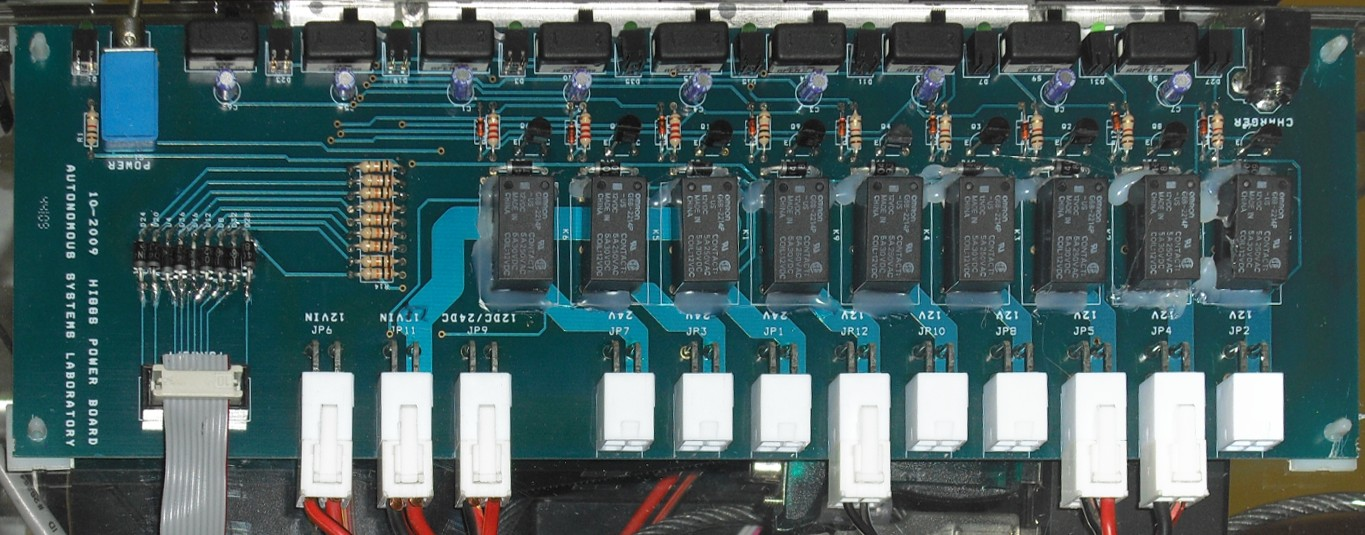
\includegraphics[width=0.5\textwidth]{figures/device_photos/powerboard.jpg}
\caption{Power board.}
\end{figure}

\begin{figure}[ht]
\centering
 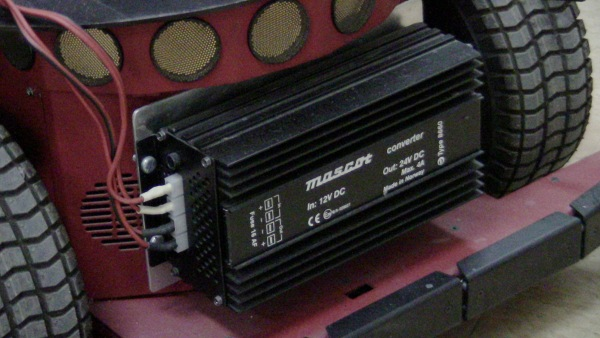
\includegraphics[width=0.5\textwidth]{figures/device_photos/converter.jpg}
\caption{12V to 24V converter.}
\end{figure}

\begin{figure}[ht]
\centering
 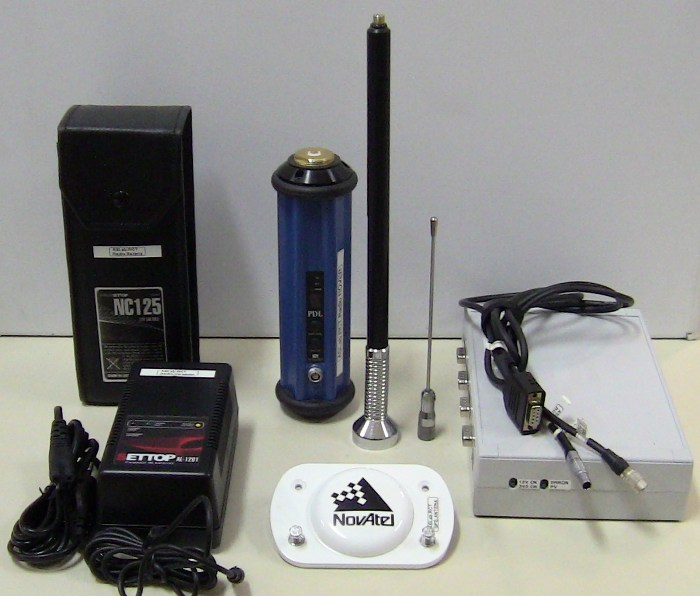
\includegraphics[width=0.6\textwidth]{figures/device_photos/gps_rover.jpg}
\caption{Differential GPS set. Rover station parts.}
\end{figure}

\begin{figure}[ht]
\centering
 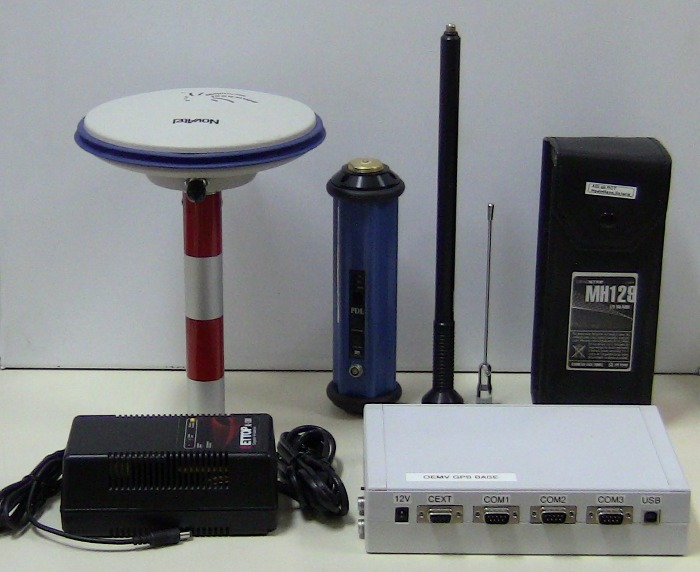
\includegraphics[width=0.6\textwidth]{figures/device_photos/gps_base.jpg}
\caption{Differential GPS set. Base station parts.}
\end{figure}

\begin{figure}[ht]
\centering
 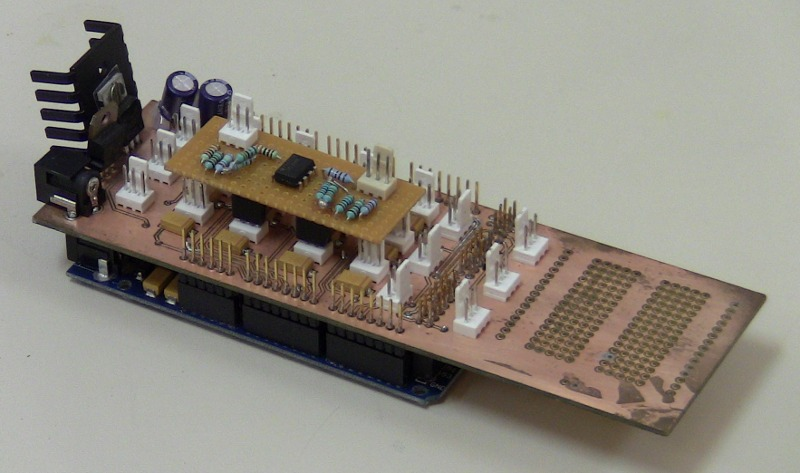
\includegraphics[width=0.5\textwidth]{figures/device_photos/ioiv.jpg}
\caption{Input/Output board: Arduino.}
\end{figure}

\begin{figure}[ht]
\centering
 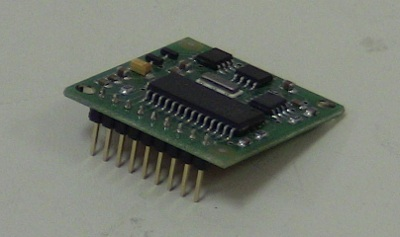
\includegraphics[width=0.3\textwidth]{figures/device_photos/compass.jpg}
\caption{Compass.}
\end{figure}

\begin{figure}[ht]
\centering
 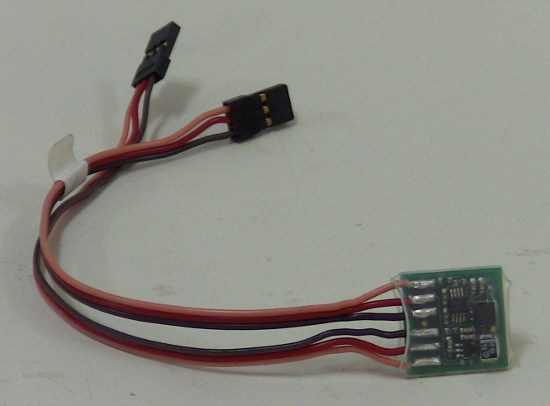
\includegraphics[width=0.4\textwidth]{figures/device_photos/accel.jpg}
\caption{Accelerometer.}
\end{figure}

\clearpage


\subsection{Data connection diagram}

\begin{figure}
\centering
 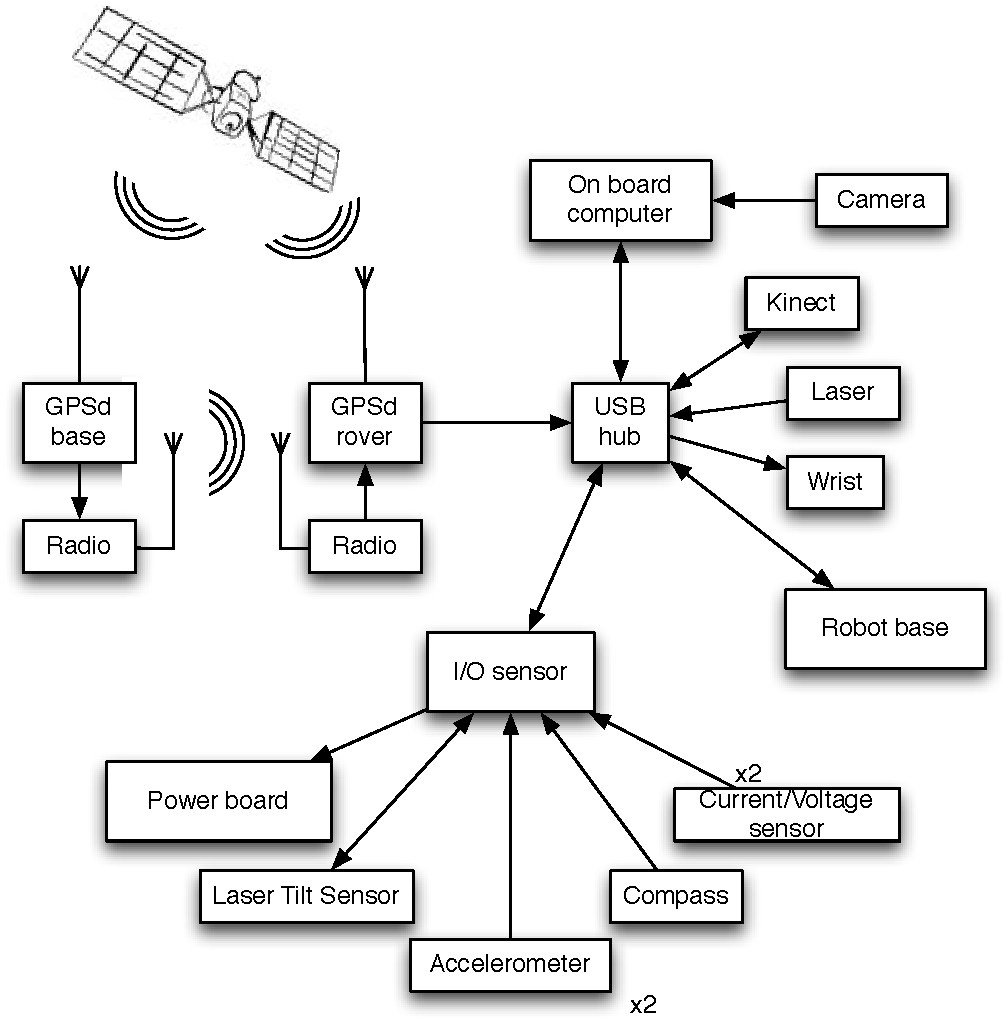
\includegraphics[width=\textwidth]{diagrams/RCT_datalines.pdf}
\caption{General data connection diagram}
\label{fig:higgs_data_connections}
\end{figure}

Arrows indicate the direction of valuable information flow.


\section{Basic maintenance}
\label{sec:usermanual_maintenance}

There is little maintenance to do with the robot. The batteries are the most important matter to be aware, followed
by the wheels.

\subsection{Wheels}
Once every two months or so, the wheels will loose pressure
and they must be inflated evenly, this way the odometry will not loose precision. It can be noticed
when the wheels have deinflated by looking to the tread pattern: Two separate bands of moist will indicate underinflation,
one on the middle overinflation, and correct inflation when moist is evenly distributed. There is a manual pump with
manometer in the ``sala F'' closet.

\subsection{Battery management}
The robot has 3 battery packages. One of them is inside the Pioneer2AT8, the other one powers the radio receiver
for the differential GPS and the laptop has its own.

\subsubsection{Robot base batteries}
There are three lead battery packages inside the Pioneer2AT8 that powers the motors, the internal electronics and
the external power board. To access them, lift the small black lever on the back side of the robot and turn it to the left.
This will loosen the battery door. Open it to 135$^{\circ}$. You may have to pull the door up to get the door over the
bump sensors. Once it is open, pull the batteries with the black sucker, or carefully with the hands do not get yourself
pinched. When inserting the new batteries, remember that \textbf{the battery terminals go last}. Failure to introduce
them correctly will cause short circuits and damage the electronics.

\begin{figure}[ht]
\centering
 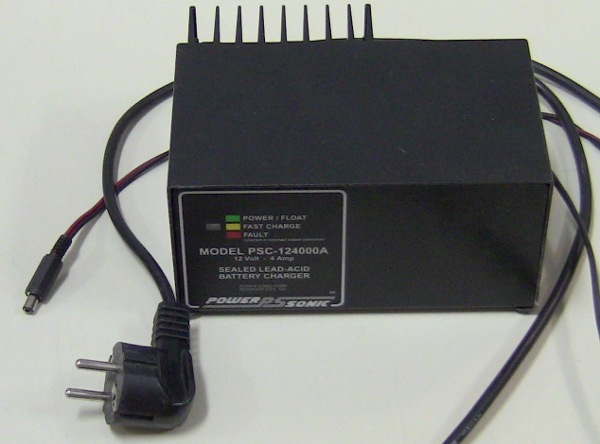
\includegraphics[width=0.6\textwidth]{figures/device_photos/rover_charger.jpg}
\caption{Robot base charger.}
\label{fig:base_battery_charger}
\end{figure}

Recommended voltage when using the batteries is between 11.5V and 12.5V. If the batteries are too low the robot
will indicate it with continuous short beeps. You can check the battery status through the battery LED in the
Pioneer2AT8 panel: Green when fully charge through orange downto 11.5V, finally red. You may find more information in the manual of the Pioneer2AT8 To keep the batteries in good
conditions, do not discharge them completely. Doing so will decrease the charge capacity. It is better to
fully charge them after each use.

To charge the batteries, connect the charger to the robot through the power jack connector to the
left of the battery door. Its charger is model PSC-124000A and is shown in figure \ref{fig:base_battery_charger}. You may leave the charger connected
for as long as you want, but remember to \textbf{switch off the robot after use}, as electricity in the
laboratory is turned off and the robot will fully discharge the batteries in this time, damaging them.

\subsubsection{GPSD radio battery}
There are two radio batteries, one for the GPS base station and the other for the GPS mobile station. Both batteries
are interchangeable, and are 8x9x23cm in size with a black leather cover.
Ni-MH batteries have memory effect, so you must discharge them completely before charging them again.
There are two chargers. you may found them in the yellow suitcase in the ``F room'' or in a white long box next to
the suitcase. Remember that the ``F room'' is the name for the ASLab cabinet in the computer rack room.
To charge it, open the battery tab and connect the charger. Press the button for discharging it fully, then wait until the
charger finishes the operation. Detailed instructions are printed on the charger. 

\begin{figure}[ht]
\centering
 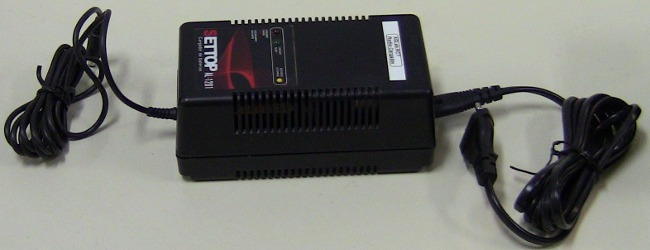
\includegraphics[width=0.7\textwidth]{figures/device_photos/gps_charger.jpg}
\caption{GPSD radio charger.}
\end{figure}

\subsubsection{VAIO laptop battery}
The VAIO laptop manages automatically its own battery. You may check its status with the command
\texttt{acpi -b} when running a UNIX based OS. On linux RTAI, ACPI is not supported by the kernel and it will not work so this command
is unavailable.

\begin{figure}[ht]
\centering
 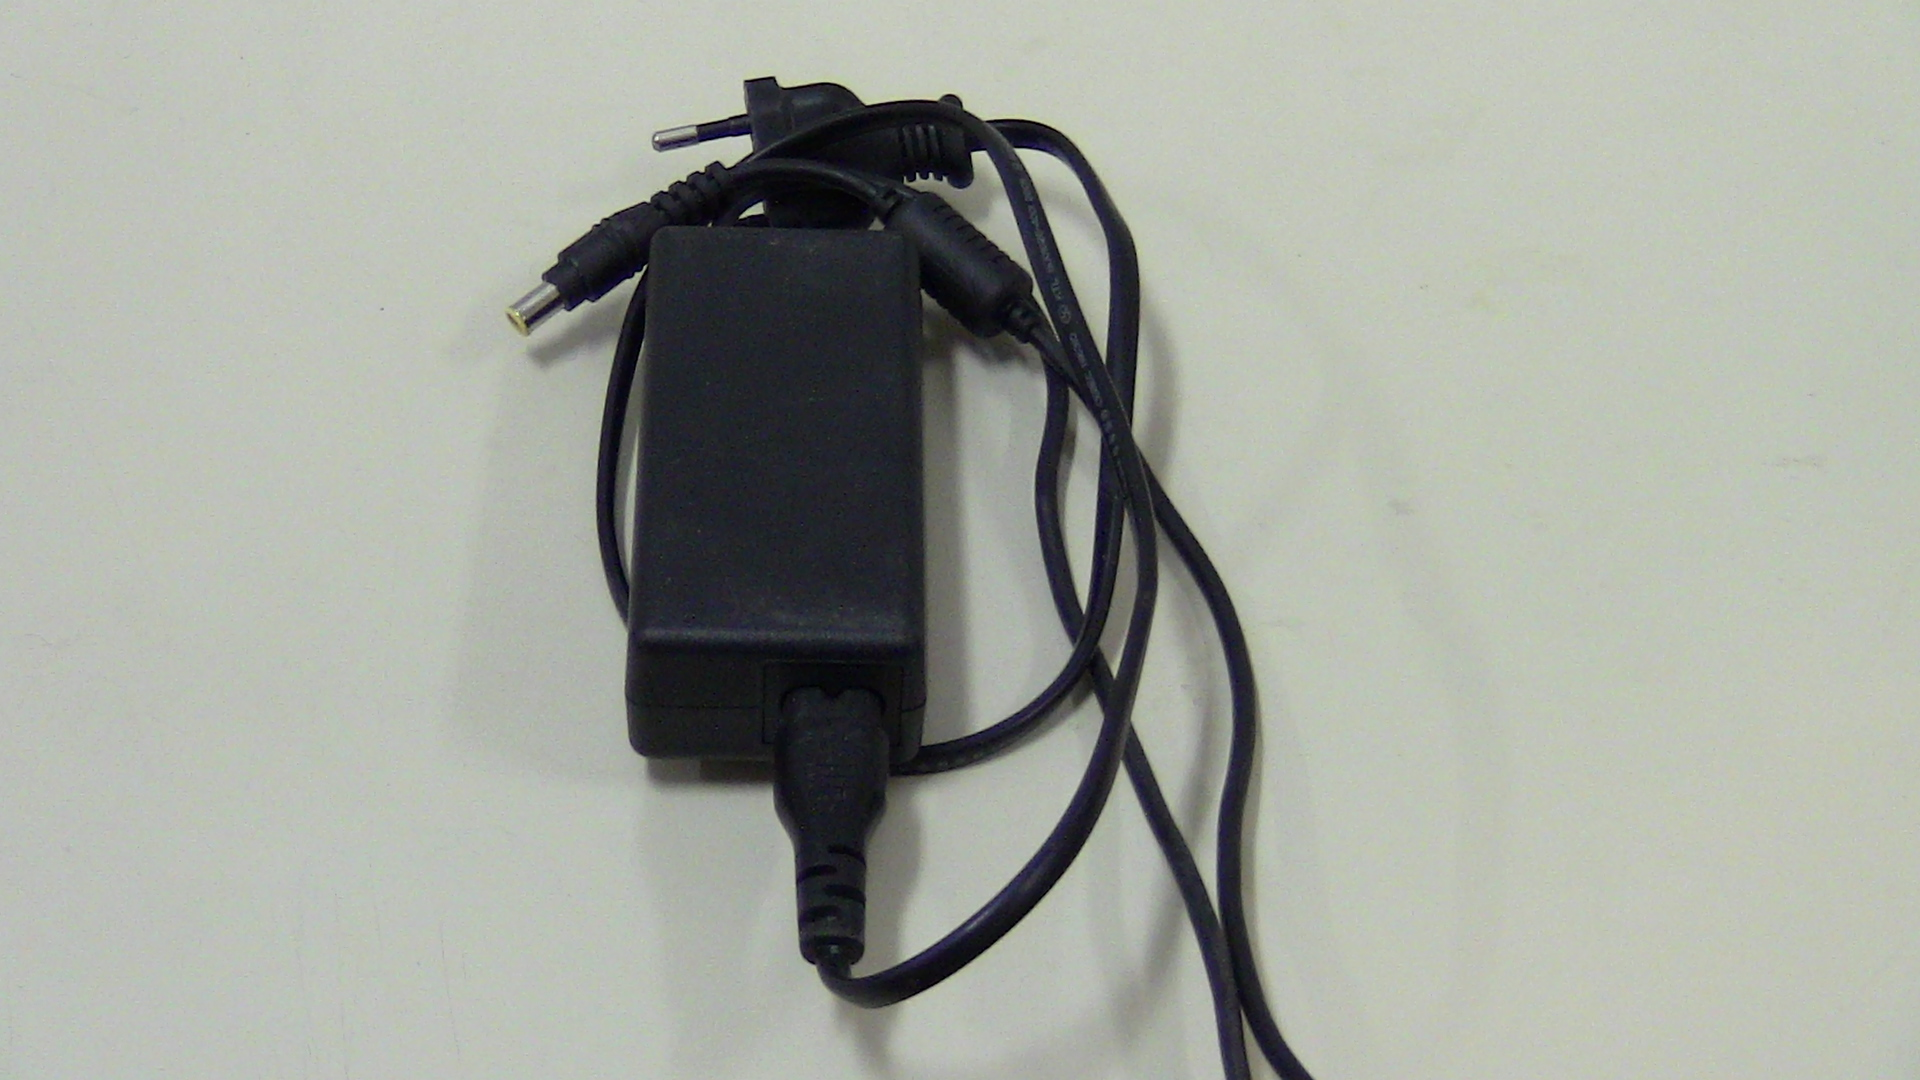
\includegraphics[width=0.7\textwidth]{figures/device_photos/vaio_charger.jpg}
\caption{VAIO laptop charger.}
\end{figure}

\subsection{Diagnostics}

\subsubsection{Power}
There are several indicators of malfunction that can ve verified in case the robot does not work properly.
In the first place, look for correct power in each device. This is how you can check it:
\begin{description}
 \item[Pioneer2AT] There is a red LED inside the Pioneer when it is powered, but can only be verified
indirectly through reflections in the methacrylate structure that covers the top hole of the base.
Alternatively, There is a dedicated red LED for this purpose in the Control Panel with the label \textit{PWR}.
\item[Laptop] The VAIO laptop lights a green LED when it is on.
\item[Laser] When it is powered on, a green LED or two orange and red LEDs will be lighted in the front of the
laser device. Green means powered and prepared, orange and red means powered and initializing.
\item[Arduino] When it is powered a little orange LED can be find behind the USB connector. A fast sanity check
is to power the arduino and the servo. If everything is OK, the Laser will rotate to look upwards in a small angle.
\item[Wrist] There is no way to verify this device externally. However, it is quite robust and will normally work
as supposed to. If everything is running ok, it will make a little calibration
movement on startup.
\item[Camera] Depends on the camera used. The black stereoscopic one has a red LED that blinks when the driver is
reading it and the Minoru3D lights up in white when the driver is reading it.
\item[GPS] There are two LEDs on the side. One of them indicates that power is OK and the other lights when enough satellites for position calculation are being tracked.
\item[Power Board] There is a green LED for the general switch and one for each device.
 \end{description}




\section{Setting up the system}
\label{sec:usermanual_setup}

Preparing the robot for operation is easy. Power it on and all systems will start automatically.
On next sections it will be discussed how to command it.

\subsection{Powering the robot}

There are three switches that must be turned on to enable the robot with full capabilities. The first one is
at the back of the robot, next to the wheels. This switch powers the Pioneer2AT8 robot base and the power board.
The power board has a general switch for all 6V and 12V devices and one more for each of these devices for manual disabling. The
power board is placed between the two big methacrylate structures. Each switch has a label with the device
it enables. The last device that should be powered is the VAIO laptop.

\textbf{Note:} The devices powered by the power board can be also disabled automatically by the
Arduino. When the Arduino is not correctly powered on, the voltage levels at its pins are undefined, and
may disable the power to some devices. Be sure to \textbf{power the arduino if you} are going to \textbf{use any other device
from the power board}.

Only the laptop is mandatory to power on. The other switches may stay off if you are not going to use the device
associated to that switch. However you will have to start at least one device to make it useful.

The Arduino does not disable any device by default.
Both the manual switches and the Arduino may force the shutdown of any device, so to use a device,
be sure that none of them disables it. The automatic switches are remotely controlled through the Arduino module.

\begin{figure}
\centering
 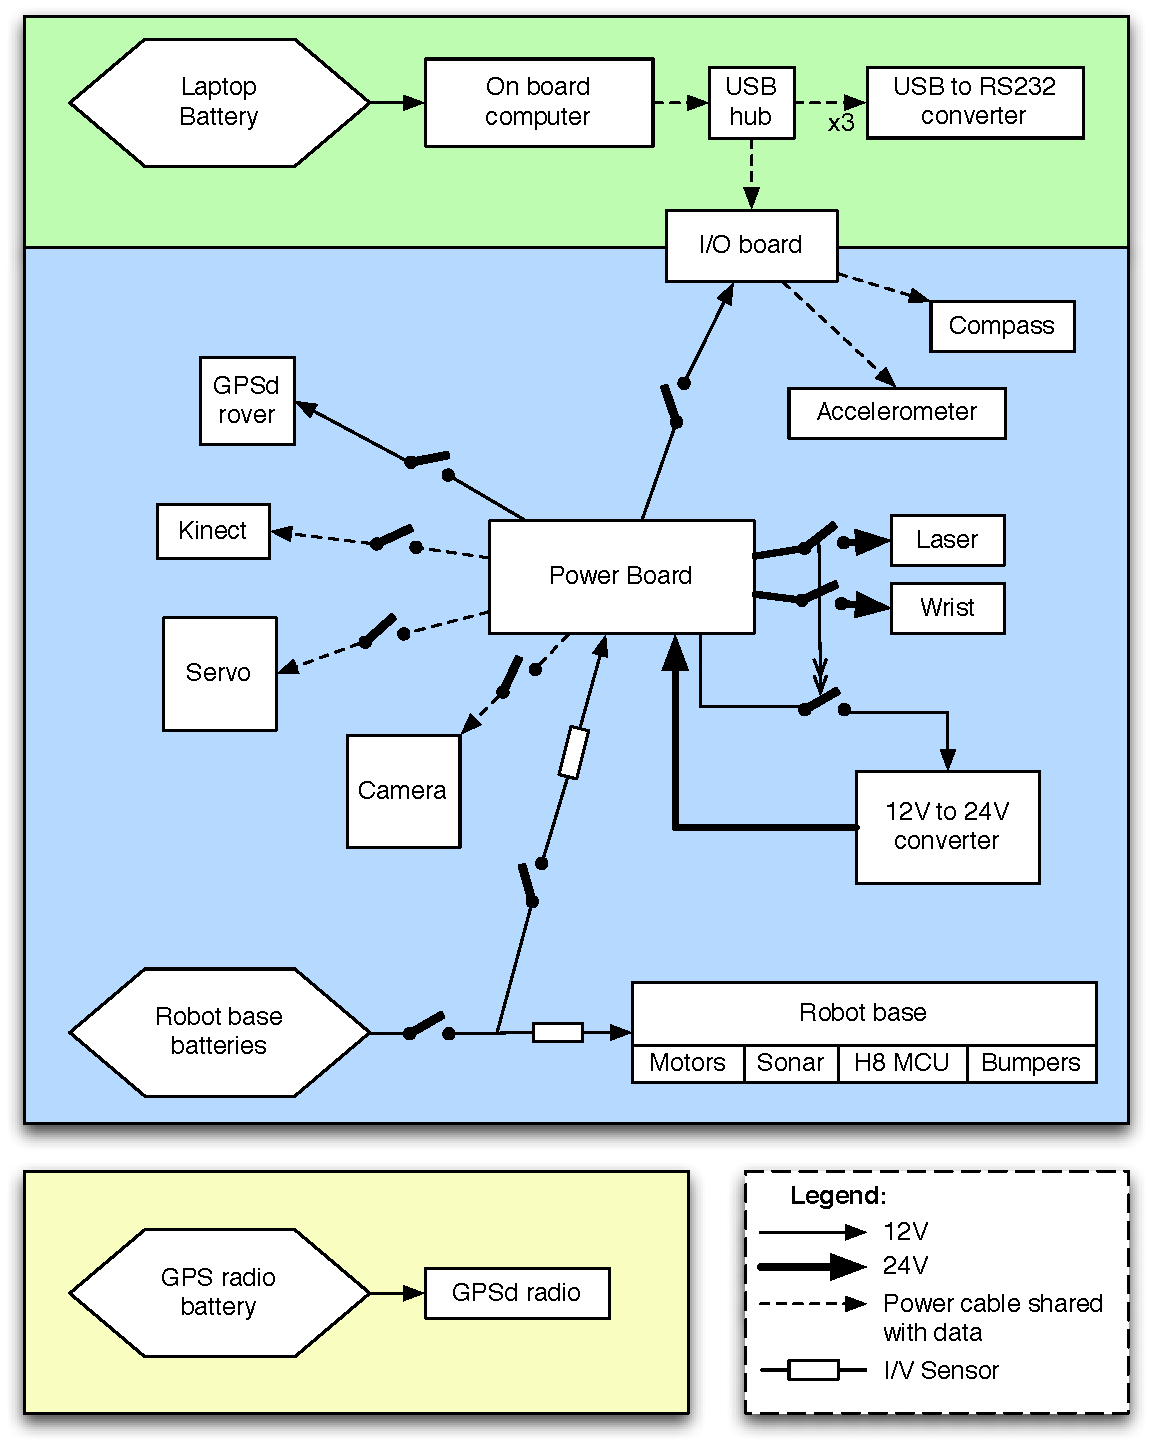
\includegraphics[width=1.1\textwidth]{diagrams/RCT_powerlines.pdf}
\caption{General power connection diagram}
\label{fig:higgs_power_connections}
\end{figure}



\section{Operating the robot}
\label{sec:usermanual_operating}

\subsection{Booting the onboard computer and choosing the OS}

The onboard computer has several operating systems installed:
\begin{description} 
 \item[WindRiver OS] \texttt{/dev/sda1} (1GB). This was once used as a testbench for the WindRiver OS. It is several years old
and is not used any more.
 \item[Windows XP Professional] \texttt{/dev/sda2} (25GB). The original Windows OS prepackaged with the laptop. The NovAtel GPSD
utilities have been installed here for quick GPS diagnostics.
 \item[Ubuntu 10.04 Long Term Service] \texttt{/dev/sda3} (14GB). This is the current
   working environment, with Real Time Application Interface (RTAI) kernel.
 \item[Fedora 13] \texttt{/dev/sda5 (29GB)}. Has the previous working environment, with CORBA modules set up and relying on the CORBA NameService in the old onboard computer. It aldo has a custom driver for supporting the FireWire camera.
 \item[Swap partition] /dev/sda6 (100MB).
 \end{description}
On bootup there is a selection of the operating system to start. It includes Ubuntu with and without real time kernel,
a RAM memory test and the other three OSs. The default OS is Ubuntu with the RTAI kernel.
Note that only the current working OS, that is, the Ubuntu with RTAI kernel, is documented here.
The other operating systems are old but kept for backup and compatibility with old software.

\subsubsection{Shutting down.}
The correct procedure to shut down the onboard computer is to log in as root and request shutdown:
\begin{verbatim}
root@higgs2:/root# halt
\end{verbatim}
Forcing instant shutdown using the power button is not recommended, however, normally there has been no problem with the OS afterwards.

\subsection{Loggin in to the onboard computer through SSH}

The Secure SHell server is run in the onboard computer by default and open to everyone that has a user account
or the root password. The root password is the same as the root password for all the computers in the laboratory.
Ask your tutor for a local account on higgs or the root password. Access can be obtained by opening a terminal
and executing the command
\begin{verbatim}
your-pc:/$ ssh account_in_higgs@higgs2
\end{verbatim} 
and root access by changing \texttt{account\_in\_higgs} with \texttt{root} or changing user to root after logging in..
If you want to execute programs that use a graphical interface, create a ssh tunnel for X with the option \texttt{-X}:
\begin{verbatim}
your-pc:/$ ssh -X account_in_higgs@higgs2
\end{verbatim}
This way the program will execute in the onboard computer and display in your local screen remotely.
In case you get this error while trying to connect:
\begin{verbatim}
 ssh: Could not resolve hostname higgs2:\
	Name or service not known
\end{verbatim}
then you have a problem with the name resolution on your computer. Copy these lines to your \texttt{/etc/hosts}
as root to solve it:
\begin{verbatim}
138.100.76.251  sagan.aslab.upm.es		sagan
138.100.76.247	higgs.disam.etsii.upm.es	higgs
138.100.76.246	higgs2.disam.etsii.upm.es	higgs2
\end{verbatim}
Now your computer knows how to translate the hostnames of the laboratory to IP's.
Alternatively, if in a rush substitute \texttt{higgs2} with its IP, as in
\begin{verbatim}
your-pc:/$ ssh local_account@138.100.76.246
\end{verbatim} 

The machine with name \texttt{higgs} corresponds to the old on board computer which was embedded inside the robot base.

Once logged in to higgs2, applications can be run as in a standard linux distribution.
Linux RTAI runs a normal kernel with standard functionality ontop of the realtime features.
For using realtime, the programs must be loaded directly into the kernel as modules. All other programs 
run in soft real time.

On bootup, the onboard computer will connect automatically to the wireless
accesspoint \texttt{aslab\_wireless}.
This accesspoint is in the same network as the  other computers. The connection is configured using the ESSID of the wi-fi hotspot and the MAC address too.


\section{Testing the CORBA modules}

The CORBA servants\footnote{A CORBA servant is an executables that provides the functionality described by the IDL file that implements.} access the NameService to publish their services\footnote{If appropriate module is installed and running.}. The table \ref{tab:names_ID_CORBA} shows the ``\texttt{id}'''s used by each module, being the ``\texttt{kind}'' parameter empty for all of them.

\begin{table}
\begin{center}
\begin{tabular}{ccc}
\textbf{Description} & \textbf{IDL} & \textbf{Name Service ID} \\ 
\hline
Camera & Camera.idl & CAMERA \\ 
I/O Board & Arduino.idl & Arduino \\ 
Robot base & Pioneer2AT.idl & PIONEER \\ 
Wrist & wrist.idl & wrist \\ 
Battery Model & BatteryModel.idl & BatteryModel \\ 
Current Monitor & BatteryModel.idl & CurrentAverage \\ 
Laser & Laser.idl & LASCOR \\ 
GPS & gps.idl & GPS
\end{tabular}
\end{center}
\caption{Names of the CORBA objects registered in the NameServer.}
\label{tab:names_ID_CORBA}
\end{table} 

\subsection{Subversion.}
The device modules have test programs that can be run either locally from the onboard computer or remotely
without needing to log in. This section and the next one are a quick guide for reconfiguring and troubleshooting easy problems with the devices. Any problem not solved here requires further understanding of the robot software mechanisms and are described in the developer manual.

The first thing to do is download the source code. Supposing you already have installed the necessary programs and libraries, type
\begin{verbatim}
svn co svn+ssh://sagan/home/svn_repositories/Higgs
\end{verbatim}
to check out the source. Again, replace \verb"sagan" with 138.100.76.251 if your hosts.conf is not correctly configured and prepend it with your user name and an @ if your server user is not the same as the local user.

There is a second repository with modules and code that have not yet been ported to the new CMake - subversion schema.
\begin{verbatim}
svn co svn+ssh://sagan/home/svn_root[/Higgs]
\end{verbatim}
If you need to search for older code there is also an obsolete CVS repository.

\subsection{Subversion directory hierarchy}

Once finished, three directories will be available:
\begin{description}
\item[\texttt{trunk}] The latest code available using the technology currently in development in the robot, which is ROS at the time of this writing.
\item[\texttt{branches}] Alternative code using other technologies, which currently is only CORBA.
\item[\texttt{docs}] The source code of this document.
\end{description}

This is the resumed directory tree inside \texttt{branches/CORBA}:
\begin{verbatim}
code
|-- LowLevelControl
|-- WorldModel
|-- batteries
|-- control_libraries
|-- devices
|   |-- arduino
|   |-- camera
|   |-- gps
|   |-- laser
|   |-- vaio_tools
|   `-- wrist
|-- idl
`-- lib
\end{verbatim}
The directories to consider when programming new clients are:
\begin{description}
\item[\texttt{code/idl}] Contains the IDL definition files of all the modules necesary for controlling the robot. You may open it for accessing the documentation for the interfaces and you will have to link to it for generating the stubs and skeletons.
\item[\texttt{lib}] C++ macro and CMake files (See section \ref{ssec:cmake}) for fast client development.
\end{description}


\subsection{Checking the environment for starting test programs.}

\subsubsection{Configuration files}

The next sections describe how to run the test programs contained in the CORBA branch for testing the devices.
The server is the onboard computer and the clients may refer both to the onboard computer or any other remote computer,
wherever the client software is running. Typically this computer will be from where the human operator is testing the modules.

Before running the test clients the configuration files must have been installed for proper operation.
Clients only need one configuration file:
\begin{verbatim}
/etc/higgs/nameservice.ip
\end{verbatim}
containing the address and port of the Naming Service that the servants are using for publishing themselves:
\begin{verbatim}
higgs2:9876
\end{verbatim}

\subsubsection{Configuring serial port links}
\label{sec:serial_links}

On the server side there are a few more entries inside \texttt{/etc/higgs}, the most important one for configuration issues being \texttt{devices}. This directory contains soft links to the character devices that represent the USB to RS-232 converters in \texttt{/dev}. The servants open these files instead of the real devices so they can be reconfigured without having to recompile. Usually you will modify these links when swapping the serial cables of the devices or changing the arrangement of the USB to serial converters. Knowing which device file goes with which device is a matter of trial and error, starting the servants and testing wether they started or not. See \ref{sec:user_log} for more information on servant logging.


\subsubsection{Starting and stopping the CORBA servants}
The servants use upstart, the standard utility in Ubuntu for booting the system and running the daemons.
You may start or stop the servants in case you need the correspondant devices, i.e. when using the laser and the robot base with ROS, or they are not automatically started on boot.

To start a servant use:
\begin{verbatim}
$ start higgs_device
\end{verbatim}
and to stop it,
\begin{verbatim}
$ stop higgs_device
\end{verbatim}
where \verb"device" is one of laser, wrist, gps, arduino, pioneer or any other available CORBA servant.

There is one more daemon, the CORBA Naming Service, which opens the port 9876, It is always running and does not interfere with the devices.

\subsubsection{Logs and troubleshooting}
\label{sec:user_log}
Servants print their output to a log file in the on board computer placed at \texttt{/var/log/higgs}. You will have to consult these for debugging problems with the servants such as not starting, setting the device file and checking overall status.

\subsection{I/O board}
The next procedure is standard on all modules.
Enter the directory \\ \texttt{\$(HIGGS\_ROOT)/branches/CORBA/code/devices/arduino/client}.\\
Be sure to have the complete source tree, at least the code subdirectory, as many methods rely on files situated back in the tree.
Run:
\begin{verbatim}
cmake .; make
\end{verbatim}
This will generate the CORBA stubs and headers and then compile the client code. The binary \texttt{arduino\_client} will appear. Run it to read the parameters of the devices attached to the I\/O board and set or reset some of the devices.

\subsection{GPSd}
You may want to test the full GPSd equipment with differential corrections or only the rover part. The differential readings may not work in the campus because of interferences in the environment that blocks radio communications between the base station and the rover.

\subsubsection{Rover}
In the first place check that
 the serial cables are correctly installed. The USB to RS232 converter should be attached to the port labeled COM1 in the GPS electronics box. Turn on the GPS switch on the powerboard. Now to the software part: Go to \\ \texttt{\$(HIGGS\_ROOT)/branches/CORBA/code/devices/gps/src} and run \\
\texttt{cmake .; make}. Run \texttt{gps\_client}. A command line menu will be printed form where you can check the satellites used in the solution, the current position and speed, the standard deviation for the position and the type of differential corrections used, if any.
This will give you the GPS calculations without differential corrections. Set up the base station to improve precision.

\subsubsection{Receiving differential corrections from the base station}
The software part is the same as in the Rover part, with the standard deviation reducing to 0.02m or so if the differential correction is working. The preparation of the base station follows.

Go to the ASLab closet and locate a yellow bag. Take out the black leather battery, the blue radio transmitter with the antenna, the white box housing the electronics and the cables. The GPS antenna is located on the roof with the coaxial cable hanging down the facade to the back of the room where Higgs lives. Open a window and take it inside. Beware of your workmates in winter! Connect it to the electronics box. Power the electronics box with 12V, for example using Higgs charger, and the radio transmitter to the battery pack using the appropriate cable. Finally connect the electronics box to the battery pack with the serial terminal attached to COM2. The battery pack is internally wired to connect the serial data and the power to the cable attached to the serial transmitter. Press power in the serial transmitter. After a few minutes, the Tx led should start blinking every second. This is the indication that the differential readings are being transmitted.

In the \textbf{rover part}, attach the three terminal cable to the blue radio receiver, the battery pack and the COM2 port in the rover GPS electronics box. Press the power button in the radio receiver and proceed as in the rover section.

\subsection{Laser}
Procedure is similar to the I/O board one. Go to \\ \texttt{\$(HIGGS\_ROOT)/branches/CORBA/code/devices/laser/src}
and \\ \texttt{cmake .; make}. \texttt{laser\_client} will be generated. Power the laser in the robot, wait for it to go green and some more seconds for the laser servant to start up, and run the client. A list with the distances of the latest reading will be printed to the console.

\subsection{Wrist}
Again, the procedure is similar, only in this case the device is an actuator and so does not give sensor readings but obeys commands. Turn on the switch for the wrist and wait for a little calibration movement that indicates that it is ready. It will move to the reset position if not there before the calibration.
Go to \\ \texttt{\$(HIGGS\_ROOT)/branches/CORBA/code/devices/wrist/src}. \\ Two clients will appear. The first of them, \texttt{wrist\_client}, will move the two axis with incremental span around ten times then stop. The second one, \\ \texttt{wrist\_client\_mouse\_grab}, will let you control the two axis with the mouse. Once running, take the pointer to the center of the window to move the wrist to the starting position, then slowly move the pointer and the wrist will follow it. The range of movements is limited by the servant for secure operation whatever the input is. However, the batteries and converter may not be able to provide the required power if too fast movements are requested.

\subsection{Robot base}
TODO

\section{Developing a client}
\label{sec:dev_client}


\subsection{ASLab client utility functions for CORBA}
The methods for initializing the CORBA infrastructure and getting the object references is quite complicated and always the same. The file \\
\texttt{code/lib/CORBA\_utils.h} contains C++ macros that ease the procedures for setting up a client, managing the errors, reading the object references from the nameserver and configuring itself for reaching that nameserver.

The typical client would be something like:

\begin{verbatim}
#include <iostream>
#include "implementationC.h"
#include "CosNamingC.h"
#include "Higgs/branches/CORBA/code/lib/CORBA_utils.h"

int main(int argc, char* argv[])
{
    CORBA_BEGIN_CLIENT(argc, argv);
    CORBA_GET_REFERENCE(module::implementation, impl, "IMPL");

    impl->do_things();

    CORBA_END_CLIENT;
    return 0;
}
\end{verbatim} 

With the correct route to \texttt{CORBA\_utils.h}. The arguments for \texttt{CORBA\_GET\_REFERENCE()} are:
\begin{enumerate}
\item \texttt{module::implementation} The type of the object to fetch.
\item \texttt{impl} The identificator desired for the reference. It should not be defined nor declared, it is done inside the macro. Remember that references are used as pointers.
\item \texttt{"IMPL"} String with the name that the object is registered in the NameServer.
\end{enumerate}




\subsection{CMake}
\label{ssec:cmake}
It is encouraged to use CMake as the tool for managing the compilation of the proyects. There is a sample CMakeLists.txt in \texttt{Higgs/branches/CORBA/code/lib}  prepared for linking the CORBA libraries and generating the necessary dependencies for compiling. Substitute \texttt{\_module} with the name of your module. The file \texttt{IDL\_command.cmake} defines a macro for generating and managing the sources of the IDL interfaces. Include all interfaces that you need when calling the macro \texttt{MacroGenerateIDL}.
Use the command
\begin{verbatim}
SET(IDL_DIR path/to/idl)
\end{verbatim}
pointing to higgs' idl definition files to tell the macro where to find them.





%===========================================================================
\chapter{Developer Manual}
%===========================================================================
The RCT testbed has been designed and developed with the tools and libraries that are currently, as
the time of this writing, the state of the art. These tools are usually replaced by easier and more
powerful ones with time, and Higgs can benefit from these. When such a change is performed, normally
it will invalidate some of the documentation herein. Remember to write down the procedures and
descriptions to match the new devices and/or software.
When replacing a broken part, this chapter can be used as a guide for installing the new components.
The tools and libraries
in use are defined, as well as how they have been installed and configured, and a detailed description of the modules,
both hardware
and software.

%----------- 1 Mobile base ------------

\section{Mobile base}
\label{sec:devmanual_base}

\subsection{Disassembling the robot}
The main reason for disassembling the robot is to access the inside of the mobile base for repairs and updates. The remaining components can be accessed without major disassembling. The robot base has two black plates screwed to the red chassis with  a joint between them. This allows to access different parts of the robot without fully disassembling it. The front part of the robot is where the motors are placed and the inner on board computer can be fitted. No computer is currently installed inside so it will rarely need servicing. See section \ref{sec:disassembling_laser} to access it. The back part houses all power and control electronics and the batteries and can be reached disassembling the back methacrylate structure with the alluminium gantry. This is achieved by unscrewing all six bolts fixing it to the robot base. Be sure to unplug all necessary cords when taking it out. The robot base will power up but will not work correctly if the  multi-coloured ribbon cable is not properly connected to the black instrument panel of figure \ref{fig:photo_converter}.
\begin{figure}[ht]
\centering
 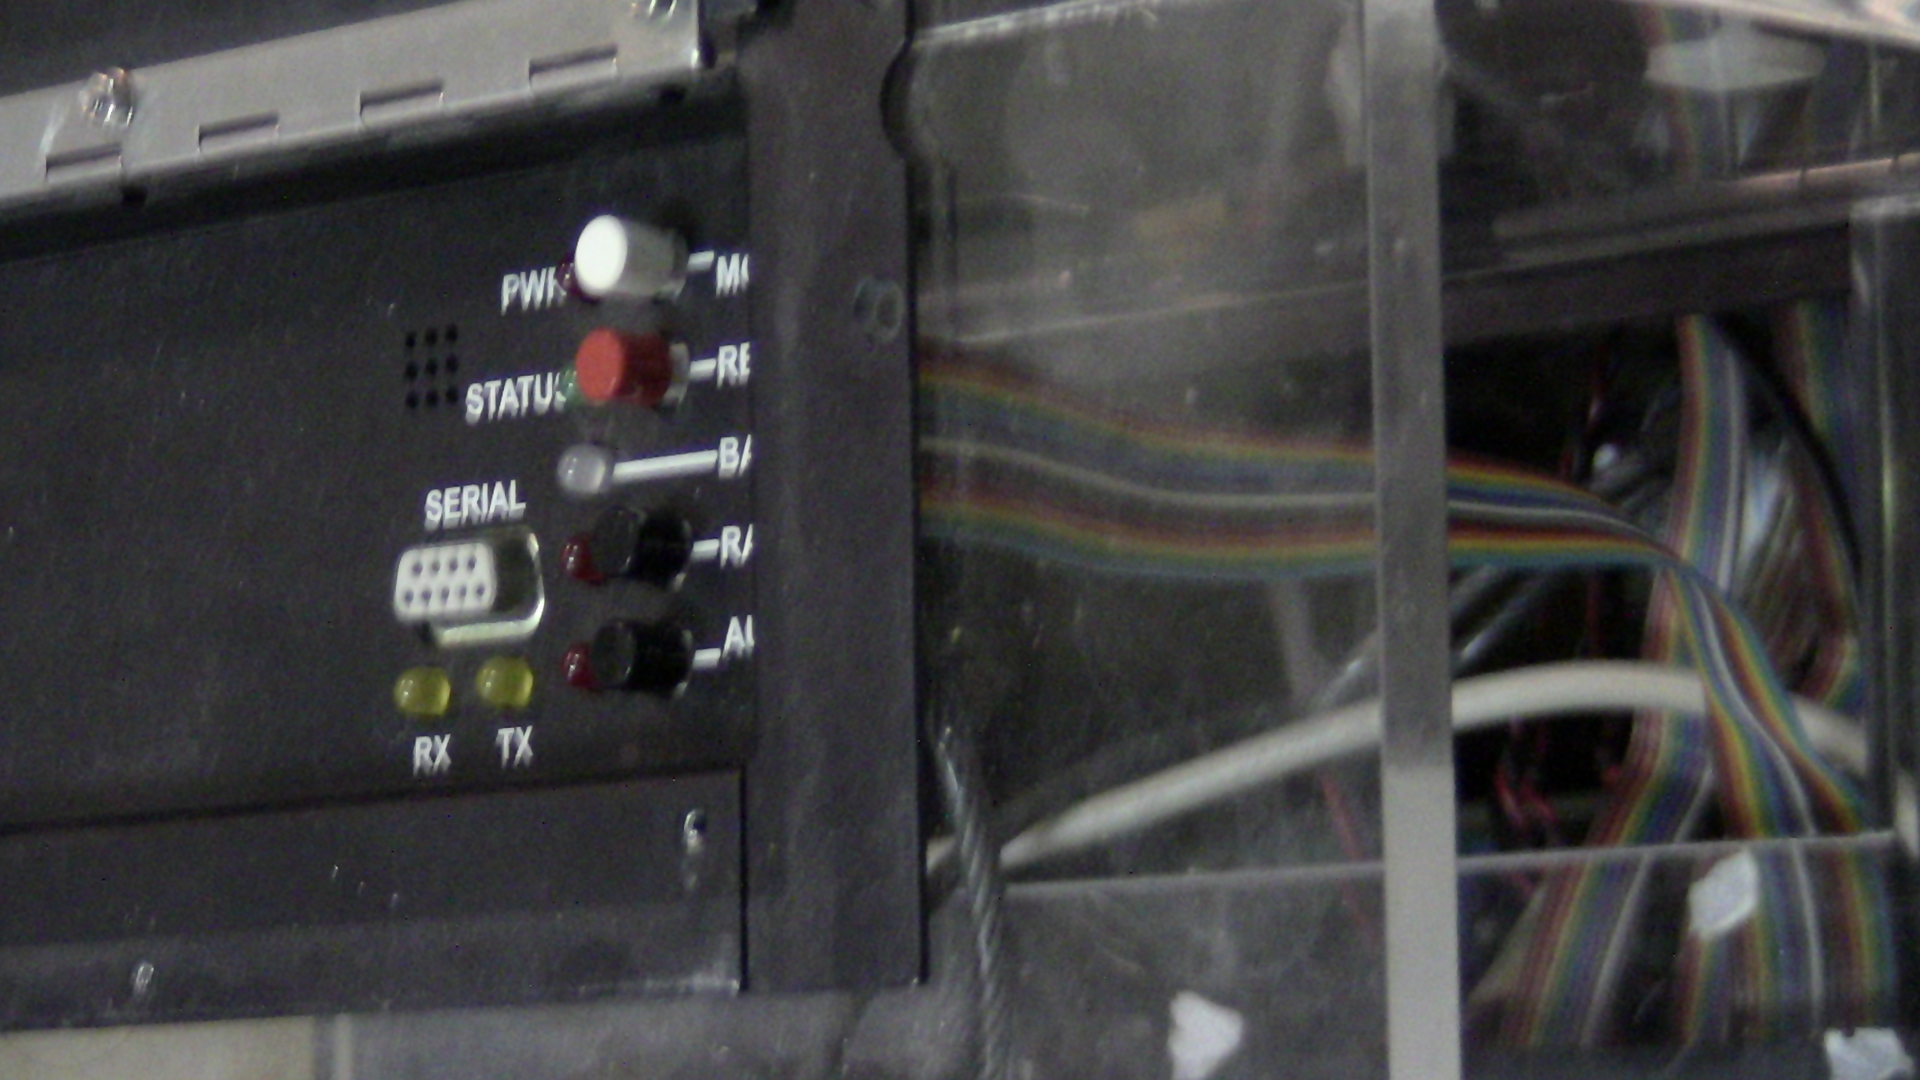
\includegraphics[width=0.8\textwidth]{figures/device_photos/multicolour_cable.jpg}
\caption{Robot base instrument panel.}
\label{fig:photo_converter}
\end{figure}


\subsubsection{Disassembling the laser}
\label{sec:disassembling_laser}
There are two ways to disassemble the laser. The first one removes the block composed of the laser sensor and the metacrylate structure that supports it. Get a number 5 allen wrench and unscrew the bolt placed under the laser, tiliting the latter upwards to reveal it. Then remove the two similar bolts on the other border of the alluminium plate that the first bolt was also holding. The methacrylate structure will be loose but do not take it off yet. Unplug the cords attached to the arduino board and the two data and power cords of the laser. Once all cables are released the structure can be lifted. Be careful not to damage the accelerometers when reassembling as its placement has been carefully crafted to fit between the laser structure and the arduino connection board. 

The second way allows for easier but more tedious disassembling. Remove the radio receiver of the GPS turning it as it was a huge bolt. Then unscrew the four bolts holding the upper methacrylate plate of the laser structure. Be careful with the weight of the devices fixed to this plate. This will leave the two walls standing to the sides of the laser. Looking from a robot point of view, the right wall can slide outwards releasing the laser from its side constraints. Take it out after unplugging the power and serial data cords. If further disassembling is required proceed as in the previous paragraph.

\subsubsection{Reaching the inside of the mobile robot.}
Once the top part of the mobile base is free from devices and structures both front and back inside parts of the robot can be reached unscrewing the littlest black bolts on the black plates. Additionally you can also remove the sonar sensors for reaching deeper inside the robot. There are four little vertical bolts inside the structure that holds each sonar array. Remove the ribbon cable prior to disassembling it.

In the back part of the robot reside the electronics in two layers. To access the bottom boards the top ones must be removed unscrewing the four small bolts situated behind the back wheels at the side of the robot and removing the sonar array so it can be slipped out.

\begin{figure}[htbp]
\begin{center}
 {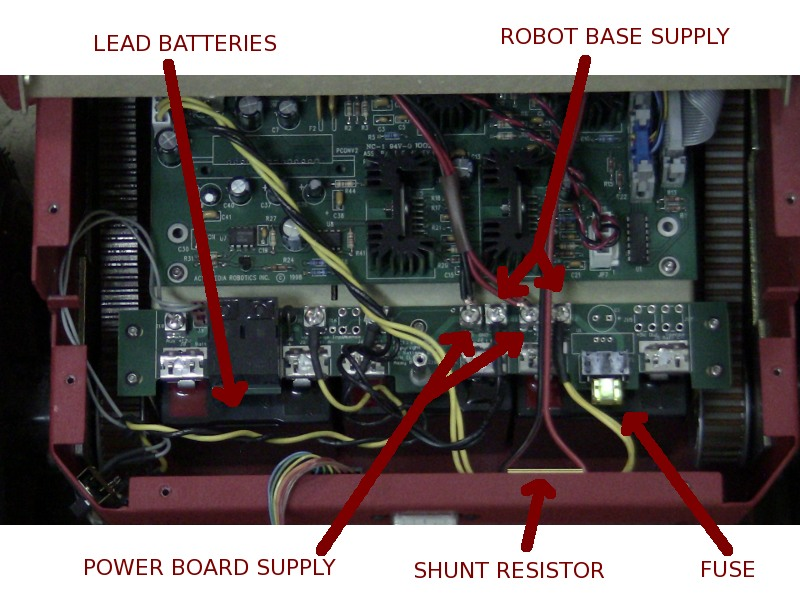
\includegraphics[width=\textwidth]{RCT_ModulesInsideRobotBase.jpg}}
\end{center}
\caption{Robot base front part disassembled.}
\label{fig:ModulesInsideRobotBase}
\end{figure}


\subsection{Firmware}
It is possible to update the firmware of the Mobile base, uploading it to the nonvolatile memory of the
Hitachi H8 microcontroller. Check the Pioneer 2 H8-Series Operations Manual. It is also possible to update
the tick count of the odometry.

%\subsection{CORBA servant}
%TODO


%----------- 2 Onboard computer ------------

\section{On-board computer}
\label{sec:devmanual_pc}

The onboard computer is the sony VAIO laptop running tUbuntu linux 10.04 with a RTAI kernel. The older onboard computer is a GENE board that was placed inside the mobile base with its own dc/dc regulator running WindRiver. See figure \ref{fig:RCT_old_gene}

\begin{figure}[htbp]
\begin{center}
 {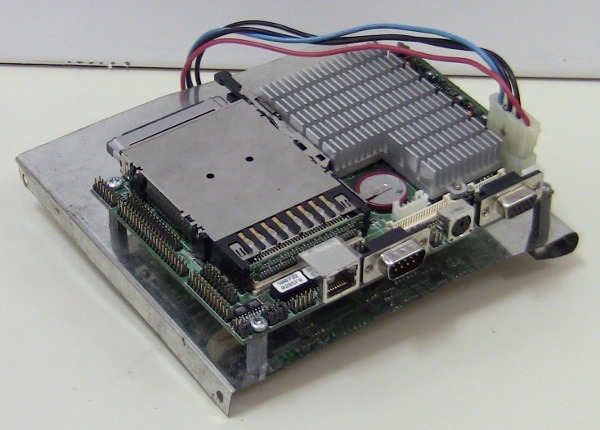
\includegraphics[width=0.7\textwidth]{RCT_ModulesVaioGene.jpg}}
\end{center}
\caption{The old onboard computer GENE}
\label{fig:RCT_old_gene}
\end{figure}

\subsection{Hubs and converters}
The onboard computer has two USB ports and one FireWire port among others. The FireWire port is used with the binocular camera. The arduino, GPS, laser, wrist and robot base all use serial RS-232 communication which is achieved using USB to RS-232 converters. There is a hub behind the power board with 4 USB ports to where the converters are plugged, either directly (two of them), with a short USB cable (i.e. the GPS) or has the converter chip embedded inside the device (i.e. the data acquisiton board). There is a lack of one serial converter for having all five devices working at the same time. Be sure to reconfigure the serial ports at \texttt{/etc/higgs/devices} when changing the connected devices, see \ref{sec:serial_links}.

\subsection{Real Time Operating System}
This section describes the steps that have been made for building and installing the Ubuntu RTAI operating system.
\begin{enumerate}
 \item Download and burn Ubuntu 10.04 LTS Desktop Edition, then install it like a standard Ubuntu installation.
The Long Term Support surname guarantees that this version will be supported for 3 years.
\item Install these packages: \texttt{libncurses-dev build-essential \\ kernel-package linux-source}
They are needed for building the kernel and generating a debian package.
\item Download and uncompress the vanilla linux kernel 2.6.32.11. The version must much exactly so the RTAI patch
can be applied smoothly. The linux kernel sources can be downloaded from \texttt{http://www.kernel.org/}.
\item Get the RTAI patch form \texttt{http://www.rtai.org/} As the time of this writing, the latest version was 3.8.1.
\item Apply the patch.
\begin{verbatim}
cd /pathtolinuxkernel2.6.32.11/
patch -p1 < /pathtortai/rtai-3.8.1/base/arch/x86/\
    patches/hal-linux-2.6.32.11-x86-2.6-0.3.patch
\end{verbatim} 
Be sure to use the patch for the exact kernel vanilla version, in this case 2.6.32.11, or errors and warnings
will arise. The \texttt{-p1} option removes the base directory form the path of the files inside the patch.
\item Configure the kernel. First, copy the ubuntu kernel config
\begin{verbatim}
 cp /lib/modules/`uname -r`/build/.config \
     /path_to_kernel-2.6.32.11
\end{verbatim} 
and run \texttt{make menuconfig} inside the root directory of the downloaded kernel sources. Look for the following options
and change them to the appropriate values: local version-append to -rtai.3.8.1-1; number of CPUs to 1; ACPI to no;
all power management features to no, module versioning support to yes, interrupt pipeline to yes.
The RTAI patch needs ACPI not to be supported by the kernel. As a consequence, no power management features will
work and the kernel will not be able to run the HALT instruction on shutdown.
\item Compile with \texttt{make}. This can last many hours.
\item Generate the debian package.
\begin{verbatim}
fakeroot
make-kpkg --initrd kernel_image kernel_headers
\end{verbatim} 
\item Go to the upper directory, where the packages are created, and install them with \texttt{dpkg -i *.dev}.
\end{enumerate}
Once the kernel is installed, reboot and start with the new kernel to check it con boot. Now it is time to
finish the installation compiling the realtime kernel modules and utilities.
\begin{enumerate}
 \item Go to the root directory of the RTAI source code and run \texttt{make menuconfig}. Select the number of
target cpu's with the same number as the kernel and write the path to the kernel sources.
\item \texttt{make} and as root \texttt{make install}.
\item Configure the libraries as root.
\begin{verbatim}
echo /usr/realtime/lib > /etc/ld.so.conf.d/rtai.conf
ldconfig
\end{verbatim} 
\item Add \texttt{/usr/realtime/bin} to the path of all users' .profile files.
\begin{verbatim}
 echo "PATH=$PATH:/usr/realtime/bin" > ~/.profile
\end{verbatim} 
\item Finally, check that the realtime extensions are working correctly. Go to \texttt{/usr/realtime/testsuite/kern/latency}
and run \texttt{./run}. If realtime is correctly installed, the last column should be all zeroes after 2-3 minutes.
\item Optionally, if space is low remove the packages and the source for the kernel and patch, or only the object files
with \texttt{make clean}.
\end{enumerate}


\subsection{OS Tweaks}
There are some modifications to be done to the Operating System to have Higgs' modules running flawlessly.

There must be a username called higgs and it must be a member of the dialout
group. Note also that by default the iptables firewall is enabled on many
distributions and it must be configured or disabled before CORBA clients can make calls to the
servants.

\subsubsection{Kernel modules}
\label{sssec:kernel_modules}
The linux kernel loads the serial modules for the converters at startup by default, but the order in which it does it is not the same on each bootup, so the serial device links must be checked on each bootup with this setup. The modules are the FTDI driver \texttt{ftdi\_sio.ko} and the pl2303 driver \texttt{pl2303.ko}. This inconvenience has been avoided by moving the kernel file objects from their standard placement at \texttt{/lib/modules/} to \texttt{/etc/higgs/modules}. The kernel tries to load the modules but fails because it can not find them where it expects them to be. The modules are loaded with the init scripts in a determined order. The following commands as root can be used to set up this behaviour on new installations:
\begin{verbatim}
cd /etc/init.d
echo "#!/bin/sh" > load_serial_modules
chmod a+x load_serial_modules
echo "insmod /etc/higgs/modules/pl2303.ko" \
 >> load_serial_modules
echo "insmod /etc/higgs/modules/ftdi_sio.ko" \
 >> load_serial_modules
ln -s /etc/init.d/load_serial_modules \
 /etc/rc3.d/S60load_serial_modules
\end{verbatim}
Replace \texttt{rc3.d} with the runlevel the OS starts with. You may instead prefer to modify the init script skeleton and give more functionality such as removal of the modules using the standard init V procedure such that loading and unloading the modules is done with \texttt{./load\_serial\_modules start/stop}.

\subsubsection{Daemon scripts}

The onboard portable computer is running many of the CORBA modules under
Linux. The base operating system has been modified slightly to run in an
unattended fashion.

Modifications made to the onboard computer:
\begin{itemize}
 % No more, as ACPI is disabled in linux RTAI.
  \item \texttt{/usr/bin/gnome\_power\_manager} has been renamed to \\
    \texttt{/usr/bin/gnome\_power\_manager.disabled}.
   This allows\footnote{This is not valid in Ubuntu RTAI as the ACPI subsystem is not functional. It is documented here in case other OS is used.} for the computer to run while it is on batteries and the screen is down.
   Otherwise the Vaio goes into suspend mode and no process can execute.
   To read the battery life do \\ \texttt{cat /proc/acpi/battery/BAT1/state} or
   \texttt{acpi -b}
 \item \texttt{/etc/init.d} The servants are configured to be managed by upstart. The config files determine which modules to load, when to restart and where to redirect the output (logs). See section \ref{ssec:module_config} for detailed description.
 \item \emph{restart\_servants} It is possible\footnote{This is not available when running the RTAI kernel.} to restart the servants by
   pressing the eject button on the Vaio, even with the lid down. This button
   will generate an ACPI event that will be processed by \texttt{acpid} using
   the configuration file \texttt{restart\_servants.conf} which in turn will
   call \\ \texttt{restart\_servants.sh} that will force the termination of the
   servants, which will be restarted by upstart. The
   configuration and script files go respectively under
   \texttt{/etc/acpi/events} and \texttt{/etc/acpi/actions}.
 \item The output of the commands are redirected to \\
   \texttt{/var/log/higgs/\$PROGRAM.log}
   Any problem associated to the execution of the modules may be diagnosed
   inspecting the logs in \texttt{/var/log/higgs/}, where all the output from the
   programs is registered. These files may grow big, so it has been created a
   logrotate config file for them (\texttt{higgslog}) placed in \texttt{/etc/logrotate.d/}.
\item MODULES: Removed pl2303 and ftdi\_sio kernel modules. They do not load with
   the same order on each bootup, so they are manually loaded by the inits scripts as described in \ref{sssec:kernel_modules}.
   The binaries have been moved from the original location to \texttt{/etc/higgs/modules}.
\end{itemize}


%----------- 3 Common libraries and module considerations ------------

\section{Common libraries and module considerations}
\label{sec:devmanual_common}
The RCT testbed may be controlled remotely by means of procedure calls to CORBA objects.
All of Higgs devices including the base platform have a CORBA interface definition that must be
used in order to remotely or automatically operate the robot. In this section these interfaces
are described in detail.

There are additional CORBA objects running in the on board computers that whilst not having direct control on Higgs'
physical devices, they do use the devices and provide useful, well-known and proved services.

\begin{figure}
\begin{center}
 {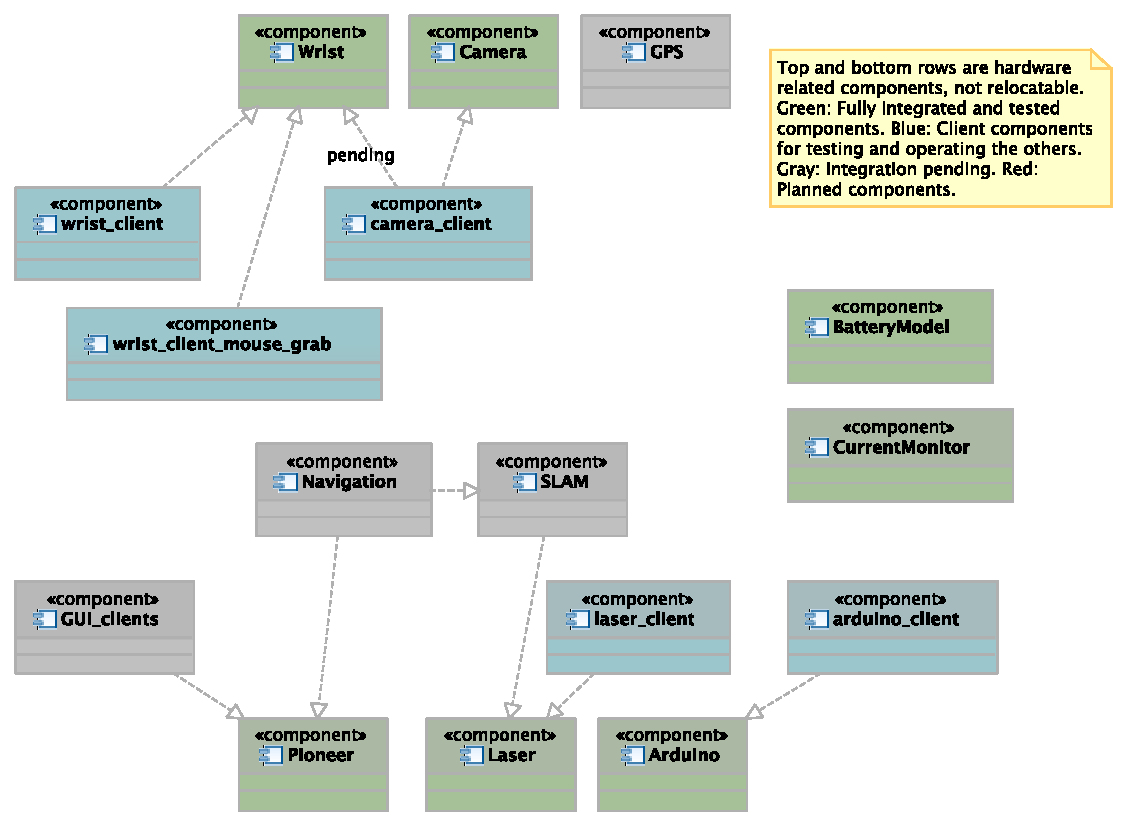
\includegraphics[width=1\textwidth]{RCT_ModulesCorbaComponents.pdf}}
\end{center}
\caption{General view of the CORBA modules in UML notation.}
\label{fig:ModulesCorbaComponents}
\end{figure}

The Java language requires that all CORBA interfaces are defined inside a module,
so all Higgs interfaces are defined inside the module \texttt{higgs}.


\subsection{ASLab servant utility functions for CORBA}
The same file \texttt{code/lib/CORBA\_utils.h} for easy creation of clients (see section \ref{sec:dev_client}) has also macros for servants.
A typical servant executable would be something like:

\begin{verbatim}
#include "implementation.h"
#include "CosNamingC.h"
#include "../../lib/CORBA_utils.h"

int main(int argc, char* argv[]) {
    CORBA_BEGIN_SERVER(argc, argv);

    implementation_t impl();
    higgs::implementation_t_var implvar = impl._this();

    CORBA_REGISTER_REFERENCE(implvar, "IMPL");
    CORBA_END_SERVER;
    return 0;
}
\end{verbatim} 
It is possible to use also \texttt{CORBA\_GET\_REFERENCE} in case other objects are needed.


\subsection{Module installation and configuration files}
\label{ssec:module_config}
The CORBA macros for the servants make use of the file
\begin{verbatim}
/etc/higgs/listen_endpoint.ip
\end{verbatim}
to configure the ip address where they should listen to, additionally to \\
the file \texttt{nameservice.ip} needed by clients.
Typically will contain the IPv4 address of the computer it is running in, in this case,
\begin{verbatim}
138.100.76.246
\end{verbatim}

Other config files are the device links at
\begin{verbatim}
/etc/higgs/devices
\end{verbatim}
Each module has this directory and the device file it uses hard coded in its source code.

Finally, they need an upstart config file. The upstart config file for the laser follows as example:
\begin{verbatim}
description "Upstart config file for the arduino servant"
author "Francisco J. Arjonilla Garcia"
start on started Naming_Service
respawn
script
	sleep 5
	date >> /var/log/higgs/laser.log
	su -l -c /usr/local/bin/laser_server higgs\
            >> /var/log/higgs/laser.log 2>&1
end script
\end{verbatim}
Other modules have different upstart config files. See each module source tree.
The Naming Service should start automatically. If not, an upstart config file must also be created for it. In either case, the endpoint must be specified in the parameters, i.e. manual execution:
\begin{verbatim}
./Naming_Service -ORBEndPoint\
    iiop://higgs2.disam.etsii.upm.es:9876
\end{verbatim}

The Java servant does not use the automatic NameService resolution mechanism provided by the C++ macros in \texttt{CORBA\_utils.h} and needs to have it specified as arguments when running it. Also, the next two lines must exist in the \texttt{.profile} file in the home directory of the user running the servant:
\begin{verbatim}
export PATH=/opt/jdk1.6.0_26/bin:${PATH}
export LD_LIBRARY_PATH=/usr/local/lib/
\end{verbatim}
Replace paths apropriately.

%----------- 4 I/O board ------------

\section{I/O board}
\label{sec:devmanual_io}

The I/O board manages the sensors and actuators that do not have a specific interface for connecting them to a computer. It has been implemented with an Arduino Mega board.
The devices controlled by the I/O board are:

\begin{itemize}
  \item Compass
  \item Accelerometers
  \item Battery sensors
  \item Laser pitch
  \item Power board
\end{itemize}

These devices are connected to the Arduino Mega commercial board through a
custom made extension board. The connector layout is shown in Figure
\ref{fig:ModulesArduinoExtensionPins}, and the connectors correspondence to
the devices in Table \ref{tab:ModulesArduinoExtensionPins}. The ribbon cable
connector  for controlling the powerboard is attached between the digital inputs 24 and 25.
Pin 0 (ground, red line on the ribbon cable) is closer to Pin22.

\begin{figure}[htbp]
\begin{center}
 {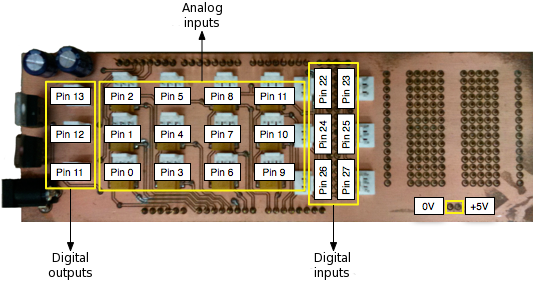
\includegraphics[width=1\textwidth]{RCT_ModulesArduinoExtensionPins.png}}
\end{center}
\caption{Connection diagram for compass board}
\label{fig:ModulesArduinoExtensionPins}
\end{figure}

\begin{table}
  \centering
  \begin{tabular}{|l|l|} \hline
    \textbf{Number} & \textbf{Device}\\ \hline \hline
    Pin0  & Not used \\ \hline
    Pin1  & Not used \\ \hline
    Pin2  & Not used \\ \hline
    Pin3  & Instrumentation current \\ \hline
    Pin4  & Instrumentation voltage \\ \hline
    Pin5  & Laser pitch potentiometer \\ \hline
    Pin6  & Motor current \\ \hline
    Pin7  & Motor voltage \\ \hline
    Pin8  & Accelerometer, X axis \\ \hline
    Pin9  & Not used \\ \hline
    Pin10 & Not used \\ \hline
    Pin11(Analog) & Accelerometer, Y axis \\ \hline
    Pin11(Digital) & Not used \\ \hline
    Pin12 & Not used \\ \hline
    Pin13 & Laser pitch servo \\ \hline
    Pin22 & Min pitch switch \\ \hline
    Pin23 & Max pitch switch \\ \hline
    Pin24 & Not used \\ \hline
    Pin25 & Compass \\ \hline
    Pin26 & Not used \\ \hline
    Pin27 & Not used \\ \hline
    Ribbon & Power board \\ \hline
  \end{tabular}
  \caption{Connector correspondence of the Arduino extension board with the
  devices.}
  \label{tab:ModulesArduinoExtensionPins}
\end{table}

\subsection{Tilt mechanism for the laser}
The laser sensor is housed inside a methacrylate structure with a joint that enables pitch movements on the laser. They are actuated by a servo placed just behind the laser, and by two end of stroke switches that limit the movements to safe values. To the left side of the laser, coaxial with the axis of rotation, there is a potentiometer that closes the loop for precise control of the rotation angle. The servo, switches and potentiometers are all controlled by the I/O board, which includes a PID control for the tilt programmed within its firmware. The details can be found in the PFC from Marcos Salom. % TODO: Falta cita bibliográfica.

Currently the PID feature has been disabled and the servo operates in an open loop fashion, using the end of stroke switches as a reference for rotation limits during initialization. The factors that motivated this decision are:
\begin{enumerate}
 \item The potentiometer is prone to errors due to mechanical hystheresis, worn out and temperature effects.
 \item There is a lot of functionlity that can be more useful than controlling the pitch of the laser. The effort has been so displaced elsewhere.
\item A better pitch angle sensor, such as an optic encoder, would justify buying a whole controlled actuator with integrated sensing and electronics.
\item The kinect sensor can partially substitute the laser.
\end{enumerate}


\subsection{Power board}
The I/O board and the power board have been connected with a ribbon cable that plugs to the doble row of pins of the extension board in the side of the I/O board. The ground connection has been stripped as the correspondent pin is not connected to ground in these pins. Common ground with the rest of the robot is achieved through the power connections that come from the batteries (Figure \ref{fig:ModulesInsideRobotBase}).


\subsection{Compass}
The compass is a solid state magnetism sensor placed next to the GPS antenna on
the aluminum bridge.
It was bought at www.superrobotica.com product reference CMPS03 S320160.
The connections are as follows, from bottom to top as shown
in figure \ref{fig:ModulesArduinoCompass}.
\begin{enumerate}
  \item VDD. To Arduino supply.
  \item SCL. To 5V with $47\Omega$ resistor.
  \item SDA. To 5V with $47\Omega$ resistor.
  \item PWM. To Arduino digital input.
  \item NC.
  \item Calibrate. To button in compass connector.
  \item 50Hz-60Hz. To GND.
  \item NC.
  \item GND. To Arduino supply.
\end{enumerate}

All connections including the calibration button are done inside the IDT
connector and protected by thermoadhesive. The button takes the calibration
input to ground when pressed.

\begin{figure}[htbp]
\begin{center}
 {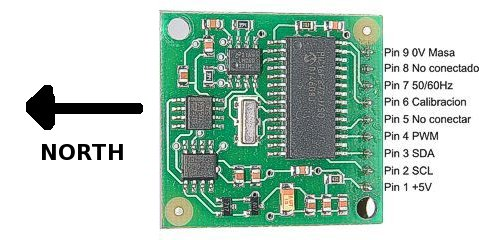
\includegraphics[width=.8\textwidth]{RCT_ModulesArduinoCompass.jpg}}
\end{center}
\caption{Connection diagram for compass board}
\label{fig:ModulesArduinoCompass}
\end{figure}

\subsubsection{Calibration instructions}
As noted in the manual of the compass, to calibrate it you have to press the
button  with the board heading perfectly well once in each direction:
North, West, South and East, no order required. It is already calibrated, so
there is no need to do it again.

The compass gives an output pulse of 1ms to 37 ms \@ VCC plus a fixed 65ms \@
GND. 1ms corresponds to $0^\circ$ and 37ms to $359^\circ$. 

The aluminum bridge does not interfere on the compass readings, but if the
robot is moving near steel structures they may be perturbed.


\subsection{Accelerometers}
There are two accelerometers encased on the same electronic board attached
horizontally with Velcro to the top cover of the robot base next to the I/O board.
They give a standard analog 0V to 5V signal and are connected directly to the
I/O board.

\subsection{Intensity/Voltage sensor}
There are two I/V sensors installed on board plus the battery status
indicator in Vaio accessible through the command line.
The two sensors can detect current and voltage of the Pioneer2AT batteries and
the instrumentation batteries. One operational amplifier per
battery has been used as a differential amplifier, as shown in Figure
\ref{fig:ModulesArduinoSensSch}. This design allows to detect small variations
in voltage of higher voltage than those of the working conditions of the
operational amplifier, specifically lower than $3.5V$, with the LM2904P
operational amplifier powered at $5V$. The voltage sensor is a scale down of the battery
voltage, which is then divided by the scale factor by software to recover the
true value. The gain is that of the differential amplifier. To read the
true current value, both the gain and the sensing resistor value must be
considered. See Table \ref{tab:ModulesArduinoDifferential} for the numerical values.
The printed circuit board is designed to fit into connectors 3,4,6 and 7 of the
Arduino extension board as an add-on module. The sensing resistors are placed
one inside the Pioneer2AT glued to the chassis under the back sonars
(figure \ref{fig:ModulesInsideRobotBase}) and the other one is in an aerial connection
on the battery cable immediately before the power board.


\begin{figure}[htbp]
\begin{center}
 {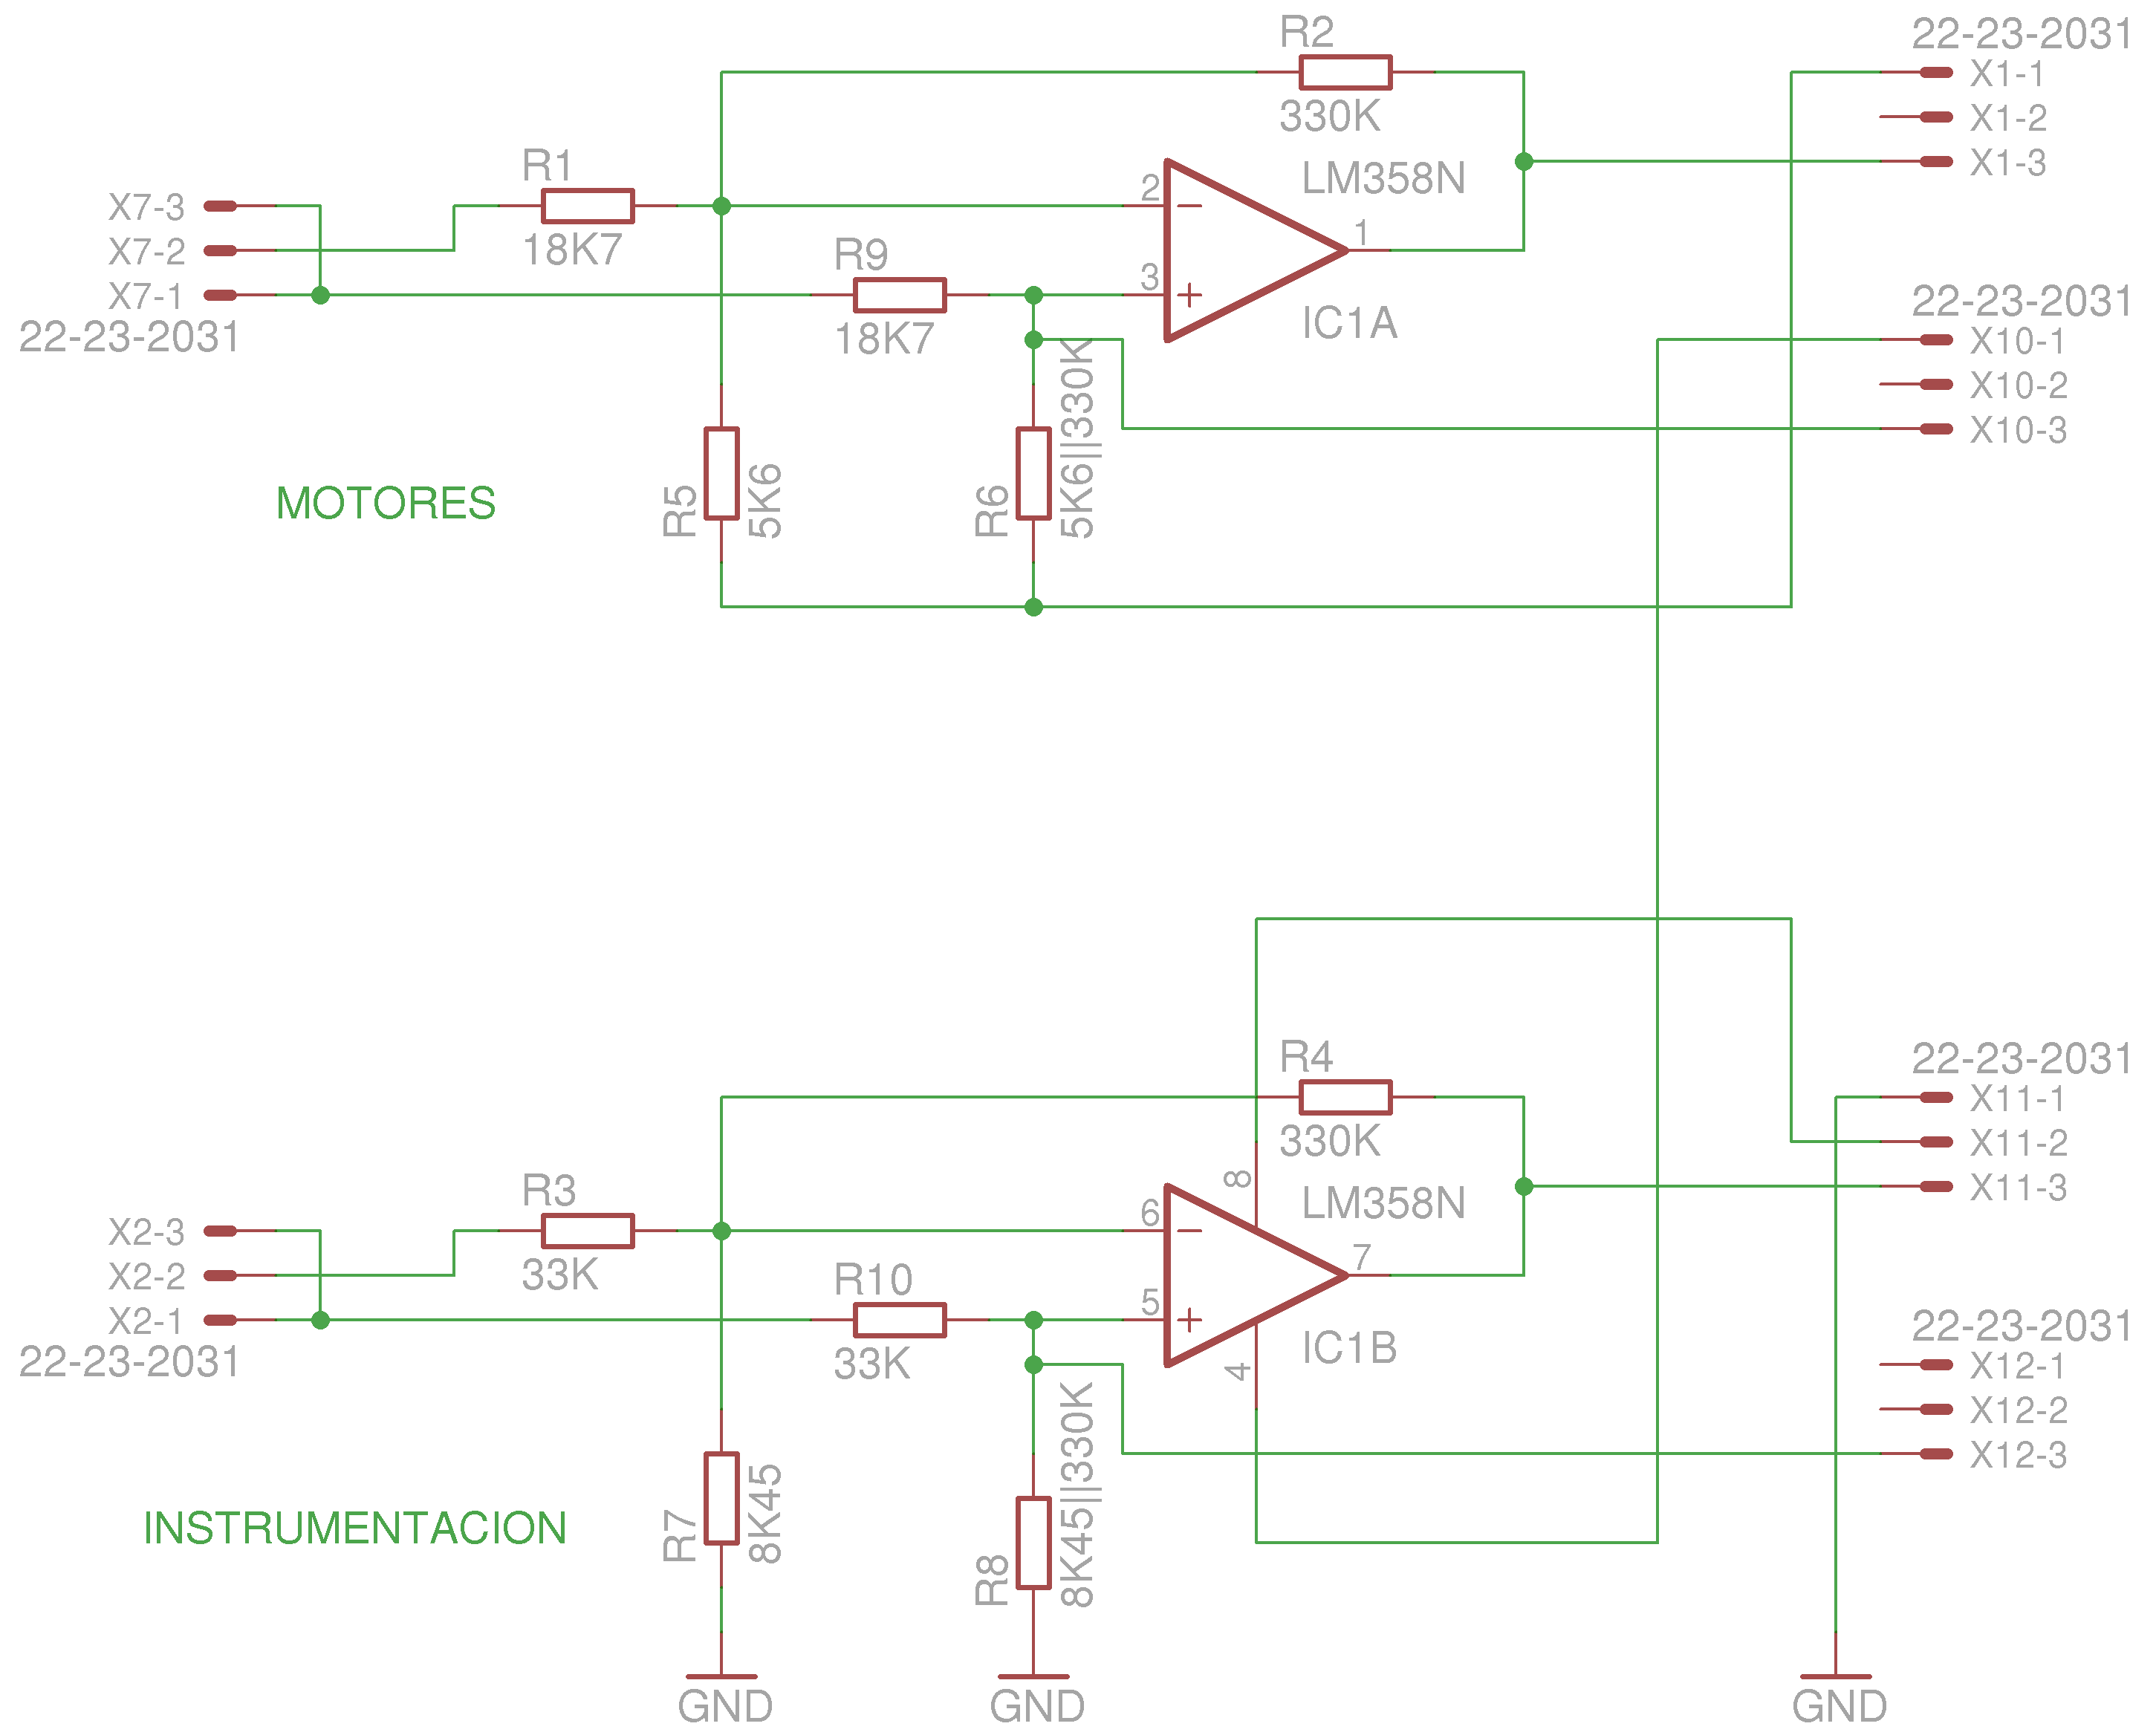
\includegraphics[width=.8\textwidth]{RCT_ModulesArduinoSensSch.png}}
\end{center}
\caption{Battery sensor schematic}
\label{fig:ModulesArduinoSensSch}
\end{figure}


\begin{figure}[htbp]
\begin{center}
 {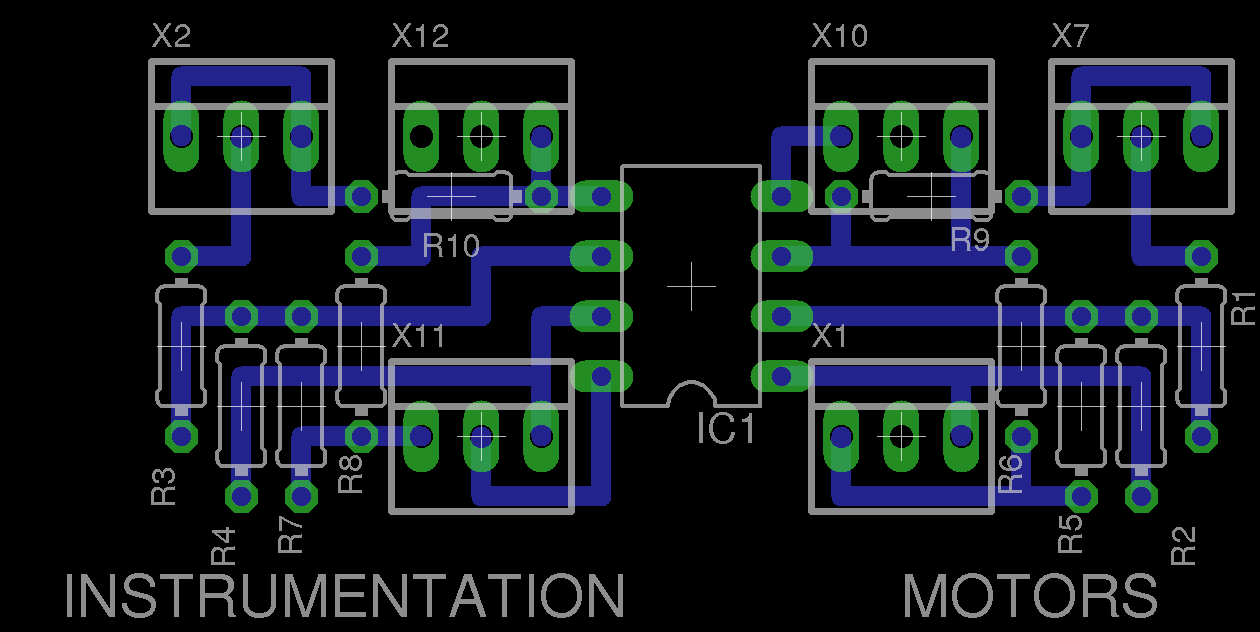
\includegraphics[width=.4\textwidth]{RCT_ModulesArduinoSensBrd.png}}
\end{center}
\caption{Battery sensor board layout}
\label{fig:ModulesArduinoSensBrd}
\end{figure}

Supposing ideal components, the output voltage given by the current sensor is
given by the formulae
\begin{equation}
U_0 = U^+\frac{R_{6}R_2}{R_9+R_6}(\frac{1}{R_1}+\frac{1}{R_2}+\frac{1}{R_5}) -
      U^-\frac{R_2}{R_1}
\end{equation} The condition that must be met for both references to be scaled down by the same
coefficient is that the relation of the resistor values
between the positive input and the negative input is
\begin{equation}
\frac{R_9}{R_6} = \frac{R_1}{R_2\parallel{}R_5}
\end{equation}
This way,
\[U_0 = \frac{R_2}{R_1}(U^+-U^-)\]
From this result we can observe that
there is great sensibility in the operation of the differential amplifiers. The
resistors from the negative input and the positive input must be of the same
value, of the same brand and of the same batch to give enough precision:
$R_9 = R1$ and $R_6$ physically being two
resistors in parallel: $ R_6 = R_2\parallel{}R_5 $.

\begin{table}
  \centering
  \begin{tabular}{|l||l|l|} \hline
    \textbf{Parameter} & \textbf{Instrumentation} & \textbf{Motors} \\ \hline \hline
	R1 & $33k\Omega$ & $18.7k\Omega$ \\ \hline
	R2 & $330k\Omega$ & $330k\Omega$ \\ \hline
	R5 & $8.45k\Omega$ & $5.6k\Omega$ \\ \hline
	R6 & $8.45k\Omega//330k\Omega$ & $5.6k\Omega//330k\Omega$ \\ \hline
	R9 & $33k\Omega$ & $18.7k\Omega$ \\ \hline
	Max sensing current & 6A & 17A \\ \hline
	Max differential input & 0.3V & 0.17V \\ \hline
	Gain & 10 & 17.647 \\ \hline
	Voltage scale factor & 0.1998 & 0.2275 \\ \hline
	Sensing resistor & $0.05\Omega$ & $0.01\Omega$ \\ \hline
  \end{tabular}
  \caption{Characteristics of the differential amplifiers for the battery
  sensors.}
  \label{tab:ModulesArduinoDifferential}
\end{table}

The current sensors will not work correctly while the batteries are charging.


\subsection{Servant and firmware}
The CORBA module for the I/O board has been written in the Java language whilst the test client in C++.
When the TurnOn and TurnOff methods are called, the appropriate device is turned
on/off and simultaneously, for the gps, laser, wrist and camera, the servant
that controls the device is killed from the arduino servant This only works if
the device servant is installed and running on the same machine as the arduino
servant, and will solve some issues on the protocol management that some of the
servants have with their device. The servant will then be restarted by the vaio
tools utility scripts.

Both the embedded program inside the I/O board and the Java servant communicate
through a USB data connection that gets converted to serial RS-232 by a FTDI chip in the Arduino board.
The I/O board starts the
communication protocol by sending all the parameters and sensor readings to the
servant, and then the servant optionally answers with the order.

The figures \ref{fig:ModulesArduinoClasses}, \ref{fig:ModulesArduinoInteraction},
\ref{fig:ModulesArduinoPC2A} and \ref{fig:ModulesArduinoA2PC} show the UML model
of the JAVA sources of the Arduino CORBA servant.

\begin{figure}[htbp]
\begin{center}
 {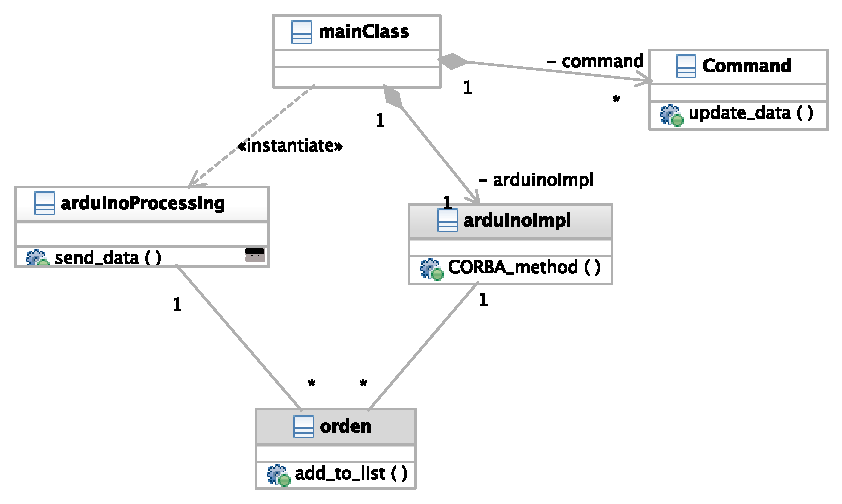
\includegraphics[width=1\textwidth]{RCT_ModulesArduinoClasses2.pdf}}
\end{center}
\caption{CORBA interface and classes used in the JAVA implementation.}
\label{fig:ModulesArduinoClasses}
\end{figure}

\begin{figure}[htbp]
\begin{center}
 {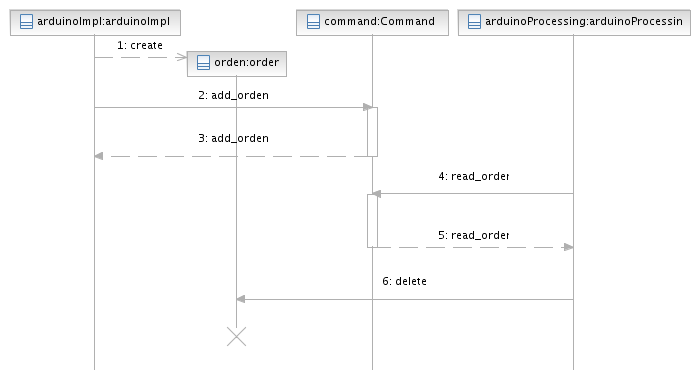
\includegraphics[width=1\textwidth]{RCT_ModulesArduinoInteraction.png}}
\end{center}
\caption{Interaction diagram for the Arduino CORBA module.}
\label{fig:ModulesArduinoInteraction}
\end{figure}

\begin{figure}[htbp]
\begin{center}
 {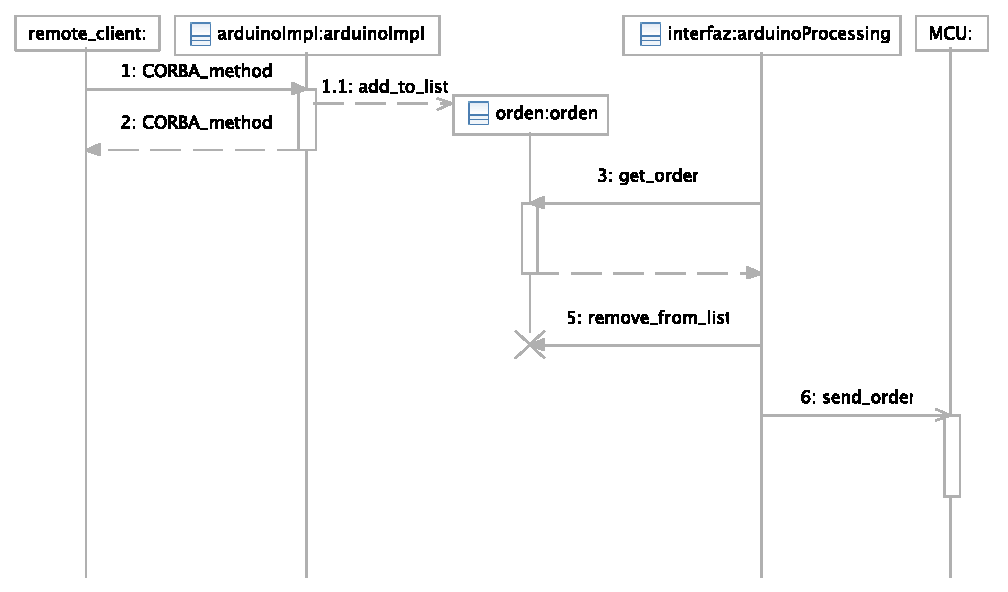
\includegraphics[width=1\textwidth]{RCT_ModulesArduinoPC2A.pdf}}
\end{center}
\caption{Sequence diagram for sending data to the i/o board.}
\label{fig:ModulesArduinoPC2A}
\end{figure}

\begin{figure}[htbp]
\begin{center}
 {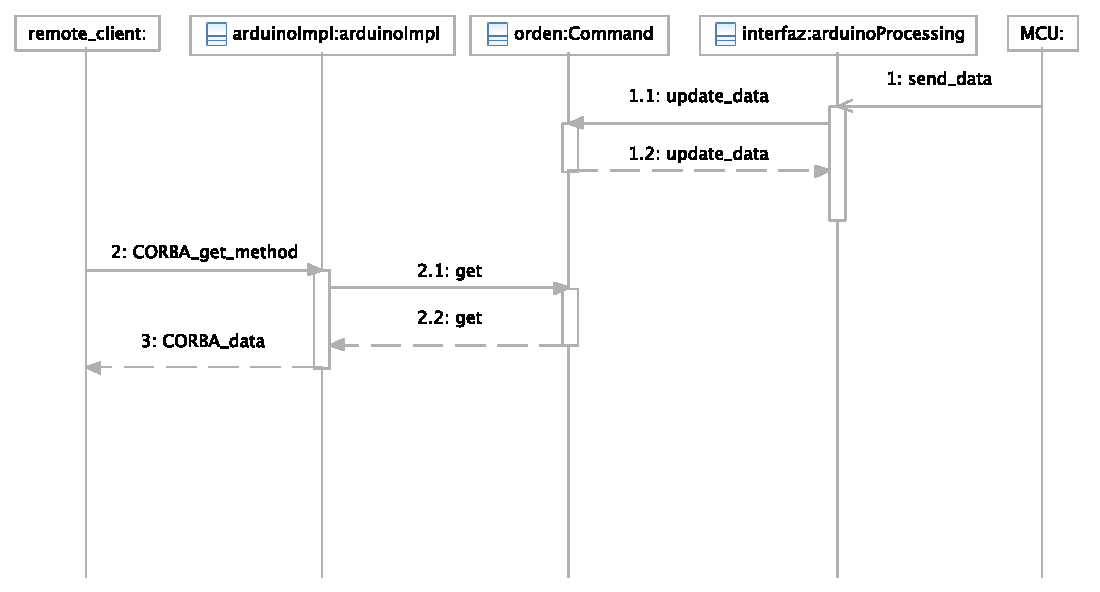
\includegraphics[width=1\textwidth]{RCT_ModulesArduinoA2PC.pdf}}
\end{center}
\caption{Sequence diagram for receiving data from the i/o board.}
\label{fig:ModulesArduinoA2PC}
\end{figure}

\subsubsection{Modifying and uploading the embedded C code}

The embedded program inside the Arduino has been developed using the official IDE
based on the \emph{processing} IDE and the libraries associated to it. A copy of this IDE
can be found inside the source code for the arduino module.

There are a few issues for remembering when installing this module on a fresh
linux installation.
The serial library RXTXcomm is included in the subversion directory \\
\texttt{svn+ssh://sagan/home/svnroot/Higgs/code/devices/arduino/lib}
The file librxtxSerial.so should be copied to \\ \texttt{/usr/\$JAVA\_BASE/jre/lib/i386} and
the three jar files \texttt{core.jar RXTXcomm.jar} and \texttt{serial.jar} to \\
\texttt{/usr/\$JAVA\_BASE/jre/lib/ext}.
Then make sure the user running the servant is in the groups \texttt{uucp}, \texttt{dialout} and
\texttt{lock}, and
that the package uucp is installed. Ensure the cross compilation environment for avr is installed. In Debian/Ubuntu these
are the packages \texttt{gcc-avr}, \texttt{avr-libc} and \texttt{binutils-avr}.

Now check for the embedded C source in the subversion directory
\begin{verbatim}
svn+ssh://sagan/home/svnroot/Higgs/code/\
devices/arduino/arduino\_embedded
\end{verbatim}
A copy of the Integrated Development Environment for the arduino is in
\begin{verbatim}
svn+ssh://sagan/home/svnroot/Higgs/code/devices/\
arduino/arduino-IDE
\end{verbatim}
or you can get the latest version from the web at \\
\texttt{http://arduino.cc/en/Main/Software}.
Start the IDE with \texttt{./arduino} and open the C source file \texttt{arduino\_embedded.pde}.
For the IDE to compile correctly, the name of the source file without the \texttt{.pde}
extension must have the same name as the directory it is in. Select the correct Board and Serial Port
\footnote{The MEGA Arduino board has an integrated USB to RS232 chip, so it will appear as a serial port
\texttt{\/dev\/ttyUSBx} when connecting the USB cable.}
under the \textit{Tools} menu, then Compile/Verify and Upload.

%----------- 5 Power Board ------------

\section{Power board}
\label{sec:devmanual_power}

\begin{figure}[htbp]
\begin{center}
 {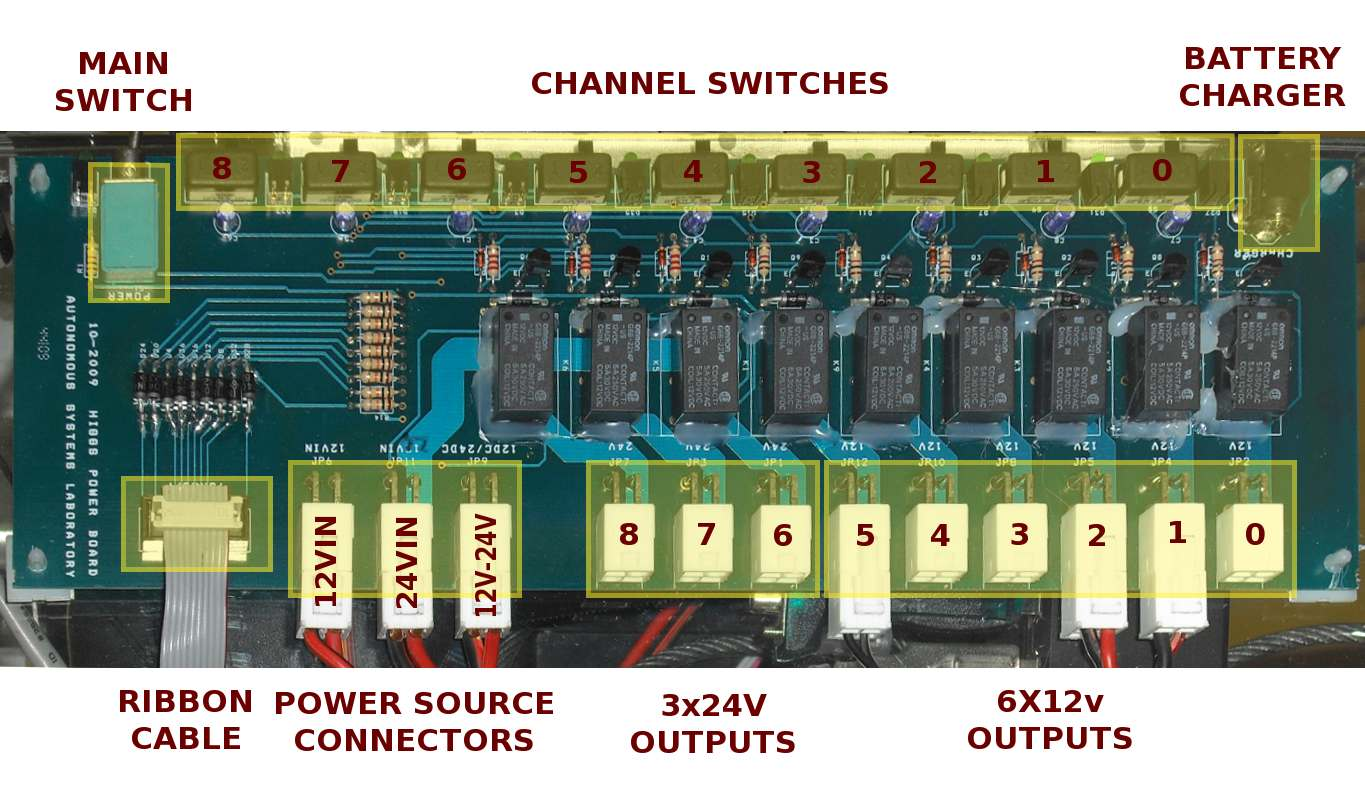
\includegraphics[width=1\textwidth]{RCT_ModulesPowerBoardPhoto.jpg}}
\end{center}
\caption{Photograph of the Power Board indicating each part.}
\label{fig:ModulesPowerBoardPhoto}
\end{figure}
The Power Board is a custom printed circuit board designed specifically for the
needs of the investigators at ASLab with which to test the algorithms in system
auto-reprogramming with partial malfunction of a robot.
The Power Board is in control of the power supply of up to nine devices in the robot. Each
of these channels may be manually shut down by means of a switch or
remotely/automatically using the ribbon cable connection to the Arduino board.
There is a LED power indicator for each channel plus and a switch and LED
indicator for all the board.
Three of the channels, the ones nearer to the general switch, can control 24V
devices whilst the other 6 are for 12V devices. On the back side there are 12
connectors, 6x12V relay controlled outputs, 3x24V relay controlled outputs, 12V
input, 24V input and a 12V output to be taken to the 12VDC to 24VDC converter
that will be powered on whenever any 24V output is enabled. Additionally, there
is a power jack connector for the battery charger\footnote{Originally there was a lead battery pack
for powering the devices on top of the robot base. This power jack connector is no longer neccessary as
the robot base has its own power jack connector for charging the batteries.}.
Thus, the Power Board needs a 12V power source and if the 24V channels are used,
it also needs a 12VDC to 24VDC converter.

\subsection{Power board pinouts}

Check figure \ref{fig:ModulesPowerBoardPhoto} for a visual description of the connectors.
The connector for the ribbon cable has the pinout indicated by table \ref{tab:ModulesArduinoPowerChannels}.
\begin{table}
  \centering
  \begin{tabular}{|c|c|l|} \hline
    \textbf{Channel / Ribbon cable pin} & \textbf{Voltage} & \textbf{Device} \\ \hline \hline
    0  & --- & Ground common \\ \hline
    1  & 12V & Not used \\ \hline
    2  & 12V & Arduino Extension Board (sensors) \\ \hline
    3  & 12V & Servo \\ \hline
    4  & 12V & Kinect \\ \hline
    5  & 12V & GPS receiver \\ \hline
    6  & 12V & Binocular Camera \\ \hline
    7  & 24V & Laser \\ \hline
    8  & 24V & Wrist \\ \hline
    9  & 24V & Not used \\ \hline
  \end{tabular}
  \caption{Distribution of devices in the channels.}
  \label{tab:ModulesArduinoPowerChannels}
\end{table}

The connectors for the devices are Molex MiniFit, RS references 670-5717 (PCB male), 679-5776
(female), 172-9134 (terminals).




\subsection{Electric interface}
The ribbon cable connector has 10 pins. Starting from pin 0, these are ground, the six
12V channels and the three 24V channels.
The channels are shut down writing a logical 0 (0V) to the corresponding pin, whilst
a 1 (5V), a high impedance or a no connection will allow for the channel to be
powered on. Both manual and remote switches must allow for the channel to be
powered on for having that channel powered.

\begin{figure}[htbp]
\begin{center}
 {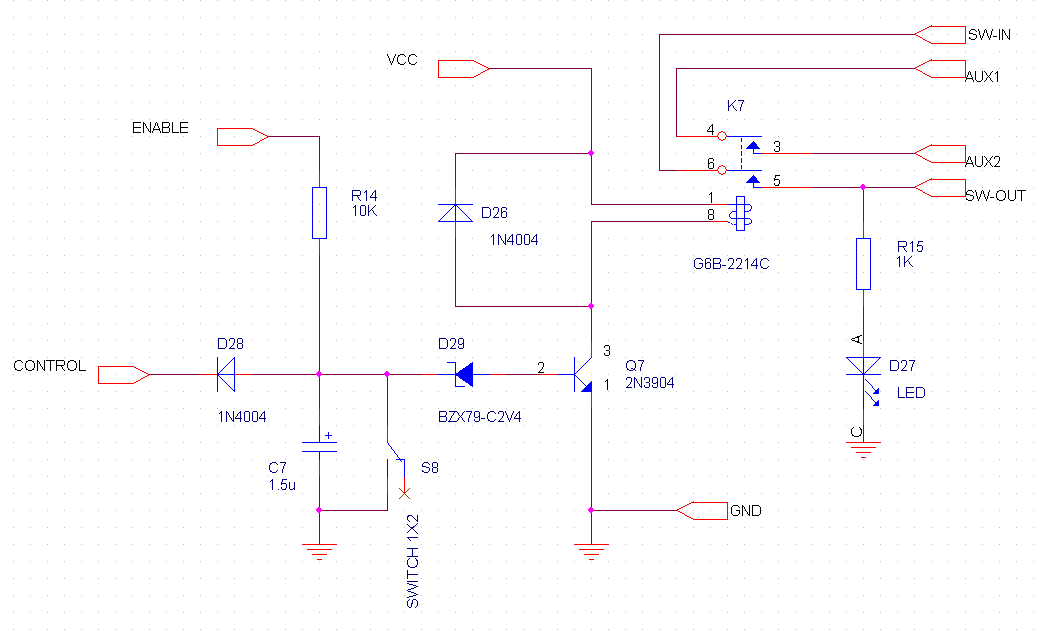
\includegraphics[width=0.9\textwidth]{RCT_ModulesPowerBoardChannelSchematic.png}}
\end{center}
\caption{Schematic for each of the channels.}
\label{fig:ModulesPowerBoardChannelSchematic}
\end{figure}

\begin{figure}[htbp]
\begin{center}
 {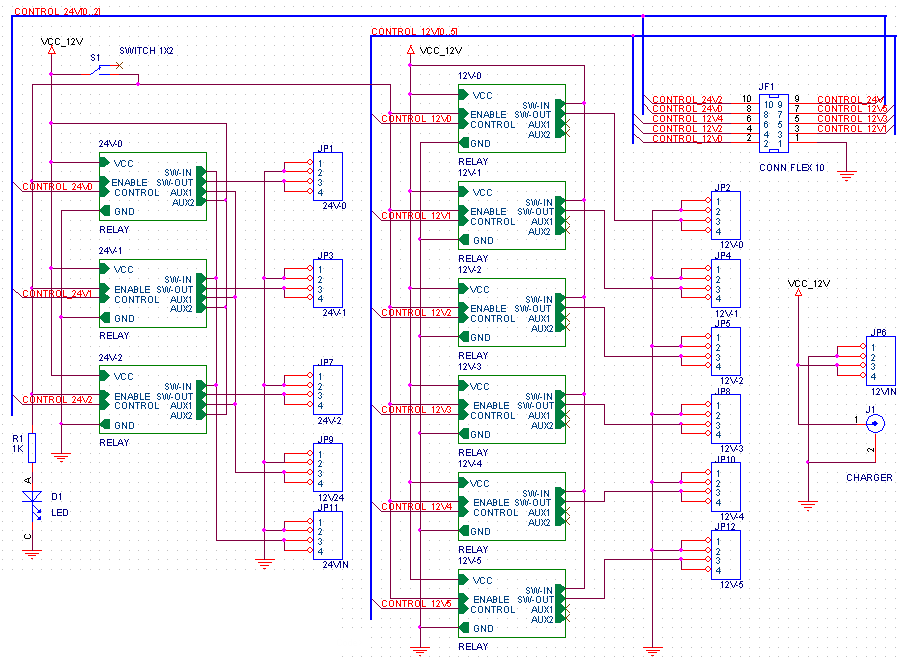
\includegraphics[width=1\textwidth]{RCT_ModulesPowerBoardBlockSchematic.png}}
\end{center}
\caption{Schematic for the Power Board.}
\label{fig:ModulesPowerBoardBlockSchematic}
\end{figure}



\subsection{Power Board Bugs}
During the design phase of the board there were some errors that passed the
internal tests. As the board was to be manufactured once, it was not
economically feasible to built it again and had to be repaired. These bugs
should be revised before sending the design in case the power board should
be manufactured again.
\begin{itemize}
  \item The holes for the diodes 1N4004 are too small. Can be repaired by
    drilling bigger holes and solding the diodes on both sides.
  \item The power jack has the positive pin disconnected. Solved with a bit of
    tin covering both the connected pin hole and the positive pin hole.
  \item The silkscreen of the connector for the 24V input is wrong, it has a
    duplicated 12VIN instead of 24VIN. Solved with a marker-pen.
  \item The relay hole distribution has the two rows of pins too far apart.
    Moreover, the coils had positive and negative pins and was not well
    documented in the datasheet, so the coil pins are swapped. Solved by
    manually separating the pins of the relays and extending the coil pins and
    securing the relays with termoadhesive. A second better approach would have been to
    solder all components on the other side of the board.
  \item Sometimes the relays do not activate correctly and/or the external radio
    emitter for the DGPS interfere with them and turns them off. Even though the
    calculations have been based on the components' specification, $R14$ and
    analogous have been reduced to $5K4\Omega$ for ensuring that enough current
    passes through the relay's coil.
\end{itemize}

%----------- 6 Wrist ------------

\section{Wrist}
\label{sec:devmanual_wrist}
The wrist \footnote{Note that even though the manufacturer calls this device
a powercube, internally we call it wrist.} is a two axis robotics kit module with pan and tilt
movements manufactured by Schunk\textregistered{}. It was
originally bought for use as the tilt mechanism for the laser, but as the center of gravity of
the laser does not match the center of rotation of either axis of the wrist, it
would be a very power hungry method for tilting the laser, given that the laser
is heavy and the power comes from a portable battery system. Moreover, one of
the axis from the wrist would be unused. It was finally decided to use the wrist
for controlling the motion of the camera, even thought it could be achieved with
a smaller controller with minor power requirements.

The manufacturer gives several interfaces for controlling the wrist: Profibus,
CAN and serial. The serial RS-232 bus was chosen over the others because of the
simplicity, the availability of drivers and the sufficient fulfillment of our
requirements. It is connected to the on board computer via a custom made
cable with an intermediate RS-2323 to USB converter. The wrist endpoint
has industry standard serial closings.
\subsection{Wrist servant}
All source code for controlling the wrist is located under
\begin{verbatim}
\$(SVN\_ROOT)/Higgs/branches/CORBA/code/devices/wrist
\end{verbatim} The programs and utilities found there include:
\begin{itemize}
\item Low level library with direct access to serial port.
\item Servant code for the CORBA object.
\item Simple CORBA client to test the functionality and status.
\item Graphical CORBA client for manually teleoperating the wrist with the mouse.
\item Compressed file with the obsolete source code for the wrist, starting
  point but fully rewritten code for the current library.
\item PDF file from the manufacturer describing the serial protocol to the wrist.
\end{itemize}

The sources are all under the \texttt{/src} directory and its documentation can be found
inside the source files.

\begin{figure}[htbp]
\begin{center}
 {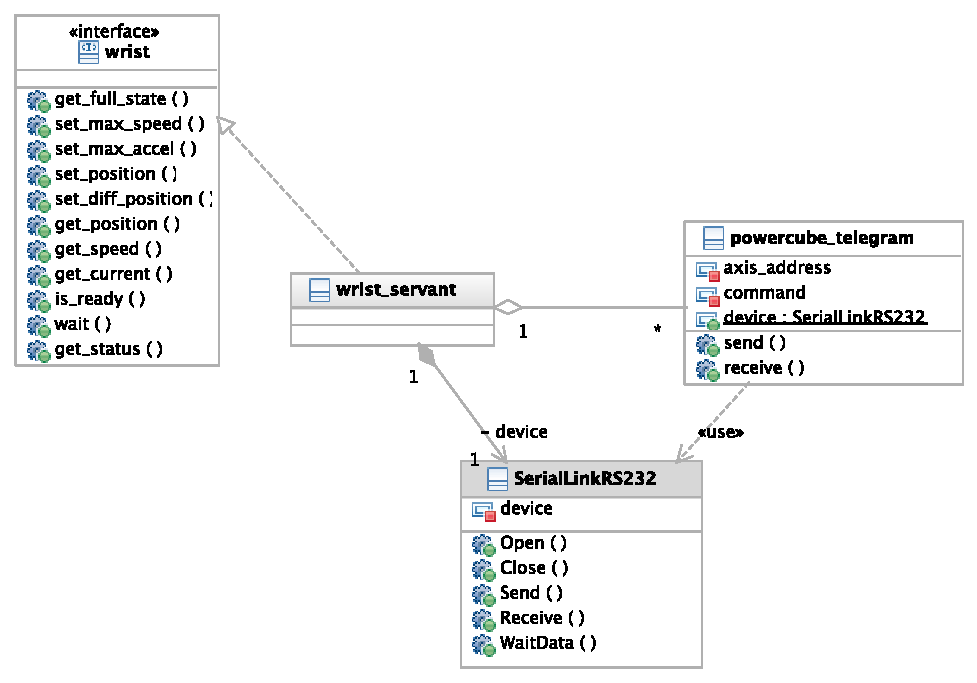
\includegraphics[width=0.95\textwidth]{RCT_ModulesWristClasses.pdf}}
\end{center}
\caption{Class diagram for wrist module and CORBA interface}
\label{fig:ModulesWristClasses}
\end{figure}

\begin{figure}[htbp]
\begin{center}
 {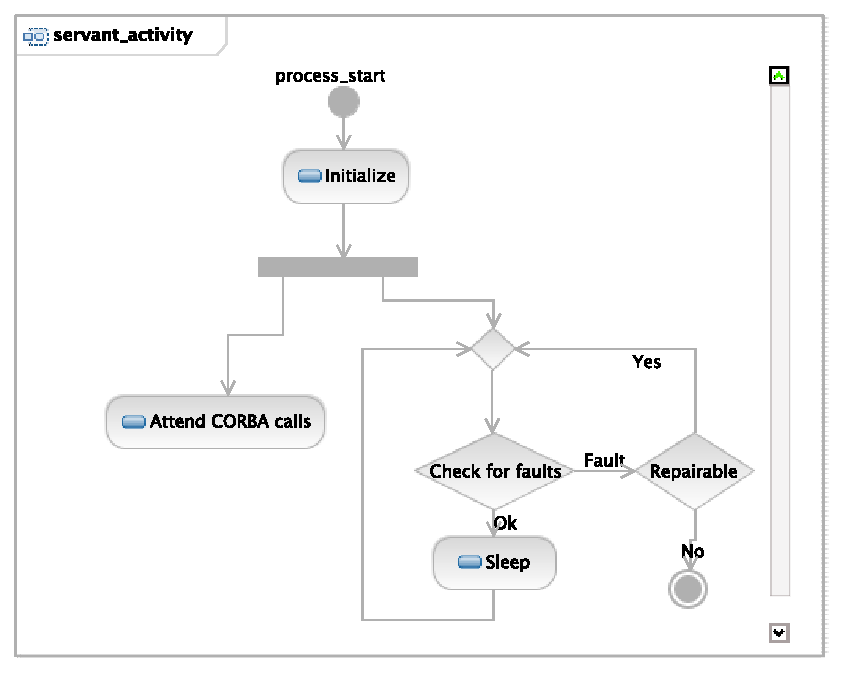
\includegraphics[width=0.95\textwidth]{RCT_ModulesWristActivity.pdf}}
\end{center}
\caption{Activity diagram for wrist servant}
\label{fig:ModulesWristActivity}
\end{figure}

When a CORBA client calls a method of this servant a new telegram is created with the parameters and format adequate to the call, passing the reference to the serial device already initialized. This telegram sends a message to the serial device and waits for the acknowledgement. This is valid for both directions of data flow. The telegram gets destroyed once the communication ends.

\begin{figure}[htbp]
\begin{center}
 {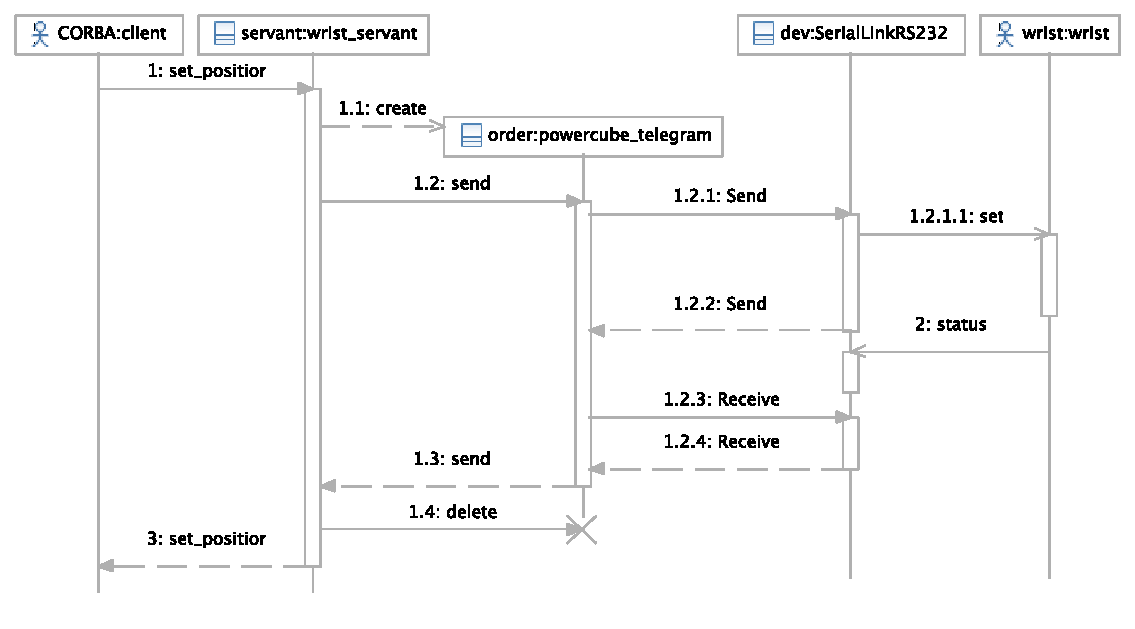
\includegraphics[width=\textwidth]{RCT_ModulesWristCorbaCall.pdf}}
\end{center}
\caption{Sequence diagram for transmitting data to the wrist.}
\label{fig:ModulesWristSequence}
\end{figure}

\subsection{Error recovery}
The wrist must be powered, as said in the official documentation, by  a 24V
power source, mobile or not. However, the fluctuations in voltage caused by
battery charge and the instant consumption of the devices make it difficult to
keep the voltage of the battery near this value. Because of this fact,
the wrist controller has been designed for high error tolerance.
A running thread in the servant polls periodically the wrist for error codes and
takes the appropriate actions when a failure is detected, as explained in each
considered fault.  These are the
possible faults that have been taken into consideration:
\subsubsection{Battery voltage out of bounds}
It has been detected empirically that the wrist will not function if the battery
voltage is under 22V or if it is over 27V, so it will not work if the battery is
either fully charged or next to empty. However, the control electronics are
still available. The status command may be issued to detect this anomaly and a
special status code will be sent by the wrist. The CORBA servant code is aware
of this fault and will abort execution to allow to complete device reset,
outputting a log and leaving the restart of the servant to the VAIO utility
programs. This fault can be prevented by periodically reading
the voltage sensor value from the I/O board, the Arduino CORBA servant.
\subsubsection{Overcurrent}
The internal current sensor will stop the axis when an overcurrent is detected
or a low voltage condition is met if the 12V to 24V converter can not supply
enough power. In this case, a reset and homing procedure is needed before
continuing operating the unit. The maximum speeds and accelerations before the
fault are saved and restored after the reset and homing procedure, but not the
position.
\subsubsection{Device not found}
This error may arise if the device is powered off, if the serial port is not
accessible or can not be found, or if the serial cable is not correctly connected.
In this case the servant will die and get restarted automatically by the init scripts.

%----------- 7 Laser ------------

\section{Laser}
\label{sec:devmanual_laser}

The data cable is a serial one prepared for RS-232 and RS-422 communications.
There is a jumper on the end connector to select which of the protocols to use.
With the jumper, RS-422. Without the jumper, RS-232. Note that the RS-422 has
not been successfully tested, maybe because the jumper should be inside the laser
connection black box instead of the serial cable endpoint.

\subsection{Laser servant}
The laser servant has been developed on top of the driver given by the people working in the mobile robotics lab. It has been modified to be able to resynchronize after a transmission error or a reboot of either the sensor or the servant. The original source code can be found in
\begin{verbatim}
$(SVN)/code/devices/laser/libreria_laser-paloma.zip
\end{verbatim}
The documentation for the Sick Laser Sensor both hardwre and protocol definition can be found under the \texttt{doc} directory of the laser sources. Inside the \texttt{src} directory you will find the modified sources for the laser driver, the servant implementation and a test client, like in other modules.


%----------- 8 Differential GPS ------------

\section{Differential GPS}
\label{sec:devmanual_gps}

The GPS module is based on two OEMV-2-RT2 receptors with capacity for Satellite Based
Augmentation System (SBAS) and Differential GPS (DGPS). Both receptors
communicate through a radio based modem capable of transmitting in half-duplex
mode through relatively long distances at 9600bps. The base radio has a transmitting power of 2W and the
rover radio 0.5W, however the latter is only used for receiving data. Both radios must be set to work in the same channel, use the button with the channel label to change it.
The electronics for each receptor have been encapsulated into plastic boxes with
these connectors and indicators available:
\begin{itemize}
  \item One double power LED indicator for checking 12V and 3.3V.
  \item One USB.
  \item Three RS-232 ports COM1 to COM3 with male DB9 connectors.
  \item One DB9 connector labelled CEXT.
  \item Power Jack connector, 12V nominal.
  \item Two TNC connectors.
  \item A reset button.
\end{itemize}
The connectors used on both base station and rover are the same. The antenna,
either the small one on the rover or the bigger circular one on the base station
is connected to the RFIN-labelled TNC connector. The other TNC connector is not
used and its purpose is to have an external high precission oscillator for the
GPS time measures. The power jack is used to power the unit. COM2 is connected
to the radio emitter/receptor for sending/receiving the differential corrections
from the base station to the rover. COM1 is connected to the VAIO laptop through
a USB to RS232 adaptor so the GPS receiver can send the position information to
the CORBA servant. On the base station, COM1 is only used when configuring the
parameters of the receiver and saving them to its internal non-volatile memory.


\subsection{Configuring the devices}
These procedures are not to be used while on normal operation of the robot. They
are only needed on first boot, then the configuration is saved permanently on
the non-volatile memory of each device. There is a little booklet inside the yellow bag where the station base is stored with the commands and parameters used by the stations.


The \texttt{minicom} command line application is best used. You may have to configure it. Open \texttt{/etc/minirc.ttyS1} and insert these lines:
\begin{verbatim}
 # Machine-generated file - use "minicom -s" to change parameters.
pu port             /dev/ttyS1
pu baudrate         9600
pu bits             8
pu parity           N
pu stopbits         1
pu rtscts           No 
\end{verbatim} 
Change the port as needed.
Run
\begin{verbatim}
 minicom ttyS1
\end{verbatim}
Now you should have access to a command line where you can send commands and check the status of the device.

\subsubsection{Base station}
Set up the base station with the RF input to the external antenna situated in the roof of the department of automatics. Get a serial cable and plug your personal computer to COM1. Start the \texttt{minicom} program to start a new session with the GPS device. These are commands were used to configure it:
\begin{verbatim}
FRESET
FIX POSITION 40.4397076 -3.6881482 744
INTERFACEMODE COM2 NONE CMR OFF
LOG COM2 CMROBS ONTIME 1
LOG COM2 CMRREF ONTIME 10
LOG COM2 CMRDESC ONTIME 10 1
SAVECONFIG
\end{verbatim} 
The meaning of the commands is as follows:
\begin{verbatim}
FRESET
\end{verbatim} 
Clears the non-volatile memory and sets the configuration to the default values. \texttt{RESET} does the same thing without clearing the non-volatile memory.
\begin{verbatim}
FIX POSITION 40.4397076 -3.6881482 744
\end{verbatim} 
This is the position measured for the base station after a period of several hours (Latitude, Longitude, Height). The command indicates the base station that it should calculate the GPS position for the corrections. All position reading after this command returns the fixed coordinates given.
\begin{verbatim}
INTERFACEMODE COM2 NONE CMR OFF
LOG COM2 CMROBS ONTIME 1
LOG COM2 CMRREF ONTIME 10
LOG COM2 CMRDESC ONTIME 10 1
\end{verbatim} 
Sets the COM2 port for sending the corrections using the message types \texttt{CMROBS}, \texttt{CMRREF} and \texttt{CMRDESC}. See the GPS manual for more information. \texttt{ONTIME 1} means to repeat the command every second. Use the \texttt{UNLOG log\_name} and \texttt{UNLOGALL} commands to stop transmitting automatic logs.  Omit \texttt{COM2} for sending the data your terminal.
\begin{verbatim}
SAVECONFIG
\end{verbatim} 
Stores the configuration to the non-volatile memory.

\subsubsection{Rover station}
Proceed as for the base station, except that the serial connection may be already available from the on board computer. In this case you may need to stop the GPS servant first to gain control of the serial device port. These commands were used to configure it:
\begin{verbatim}
FRESET
SBASCONTROL ENABLE EGNOS 0 ZEROTOTWO
INTERFACEMODE COM2 CMR NONE OFF
SAVECONFIG
\end{verbatim}
The \verb|SBASCONTROL| command line configures the GPS mobile station to use the EGNOS/SBAS satellites for better precision than GPS alone if the differential readings are not available.

\subsection{Servant}
The GPS module uses the convention for other module sources: installation and execution procedure, code placement inside the subversion repository and CORBA utilities such as in other modules are used.

The servant code uses non standard commands to receive the data from the rover station.
The commands
\begin{verbatim}
LOG BESTPOS
LOG BESTVEL
\end{verbatim} 
are sent on startup and used to retrieve the information about satellites, position, standard deviation and speed. This data is fetched by an independent thread to the CORBA one and stores it into a shared variable for the CORBA thread to read it each time a client asks for the data. There is also a timeout by which if no data is received after a fixed amount of time an error is issued.

\subsection{Radio signals and ETSII-UPM}
The ETSII-UPM is surrounded by many governmental sites. It is possible that radio transmissions with the differential corrections fail because from interference from these sites. Other investigation groups have had the same problem. In this case the dGPS will not work. Official service has anyway recommended us to use this configuration in the rover if the problem persists:
\begin{verbatim}
UNDULATION USER 0.0
FIX NONE
COM COM2 9600 N 8 1 N OFF
LOG COM2 GPGGA ONTIME logperiod
INTERFACEMODE COM2 CMR NOVATEL OFF
RTKSOURCE type any (ANY)
\end{verbatim}

%----------- 9 Binocular camera ------------

\section{Binocular camera}
\label{sec:devmanual_camera}
The binocular camera is attached to the top of the powercube, allowing for pan
and tilt movements.

The image data is transmitted in raw yuv format between the CORBA servant and the clients.

When restarting the servants, you should kill the process and call \\
\texttt{dc1394\_reset\_bus}, or else the servant will not succeed on starting
again.

\subsection{Compiling and running the CORBA module}
For installing the CORBA module on a fresh fedora linux system, you
must install these libraries which can be found in the repositories
provided by the package \texttt{atrpms}: \texttt{glut glui libavcodec} and
related. Inside the directory tree of the sources there are three scripts that help run the servant and test clients.
Compile and run the server with
\begin{verbatim}
\$ ./1-server.sh
\end{verbatim}
The test client with
\begin{verbatim}
\$ ./2-client.sh
\end{verbatim}
or, for the old client,
\begin{verbatim}
\$ ./3-client.sh
\end{verbatim}
The client runs best when configured to run with Xlib instead of OpenGL.
The user that runs the servant, higgs when running unattended, needs to be in the video group.

The source structure has not been adapted to the new tree configuration nor cmake.
\verb|idl| Contains the idl interfaces. \verb|generated| is where the skeleton and stub source files are generated to. \verb|obj| the binary files are compiled to this directory. \verb|text| contains code to test the camera without using CORBA.


%----------- 10 Other modules ------------

\section{BatteryModel and CurrentMonitor}
\textbf{Note:} Porting to the newer SVN repository is pending.

These two CORBA servants have been implemented into one JAVA binary and made an
unique module inside the VAIO on board computer. The BatteryModel is a component
that calculates the parameters related to the charge in a battery and estimates
the remaining life based on the power requirements. The CurrentMonitor is not
used in any other module but has been an utility component for developing the
BatteryModel. It periodically polls the current of the (currently
instrumentation) batteries and reports the mean consumption since it was
required to start monitoring.

Neither component reads or uses the peripherals on the computer. BatteryModel is
exclusively a CORBA servant and the clients must pass the data to it in order to
compute the estimations for the battery life, whilst CurrentMonitor is, besides
a servant, a client to the Arduino CORBA servant for reading the current values
of the batteries.

Installation of the module and automatic setup is achieved as in the other
modules.








%===========================================================================
\chapter{ASys Approach to Higgs}
%===========================================================================
\label{chapter:asyshiggs}

%\section{OASys--based Engineering Methodology Applied to RCT}

The \emph{ASys Engineering Methodology} developed in ICEA is based on the OASys ontology and has been applied to the Robot Control Testbed for its conceptual analysis. The following sections provide a description on how the different tasks were accomplished, with examples of the different workproducts obtained. The terms in italic that appear in the phases, tasks, subtasks and models descriptions are those defined in the Packages of OASys.\\

\section{RCT ASys Views Phase}
The purpose of this \emph{Phase} is to identify the different views of interest for the RCT considering the Perspective Package elements, specialised through the ASysPerspective Package concepts. \\

For example the \emph{RequirementViewpoint} especilises the concept of \emph{Viewpoint} to address the analysis of the RCT from a \emph{ASysRequirement} \emph{Concern}, to establish the different requirements to be defined in the system. Considering this viewpoint, a RCTRequirementViewpointModel can be instantiated (Fig. \ref{fig:RCTrequirementviewpointmodel}). The different concepts, relationships and attributes where chosen from the Perspective and the ASysPerspective Package. The original concepts have been ontologically instantiated into RCT related ones. For example, the concept RCTRequirement is an \emph{ASysRequirement} concern, which in turn is a\emph{Concern} from the Perspective Package. In a similar way, RCTPerformanceViewpoint is a \emph{Viewpoint}, as defined in the Perspective Package. \\

\begin{figure}[htbp]
\begin{center}
 {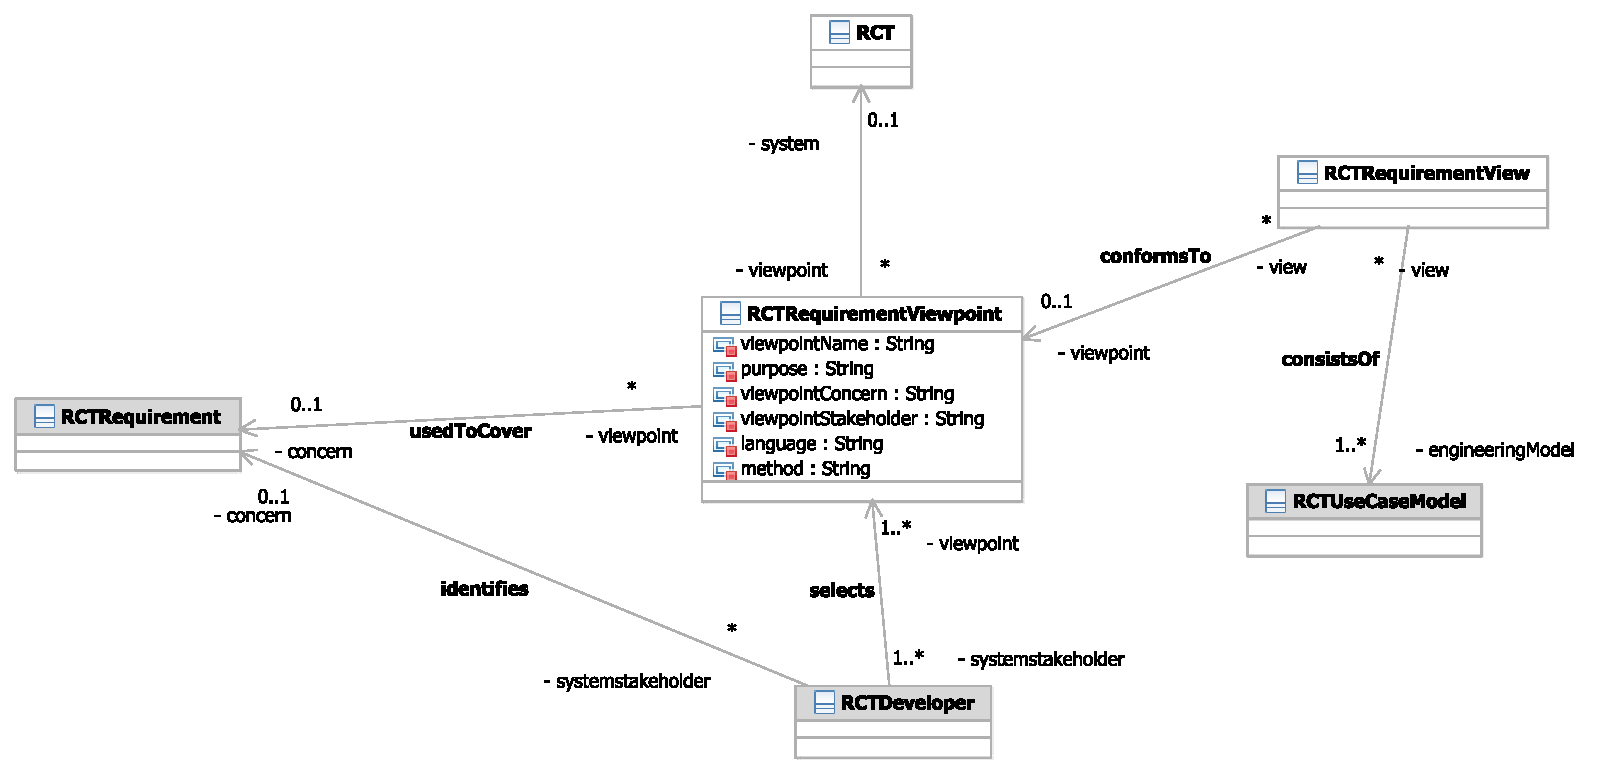
\includegraphics[width=0.95\textwidth]{RCT_RCTRequirementViewpointModel.pdf}}
\end{center}
\caption{RCT RequirementViewpoint Model}
\label{fig:RCTrequirementviewpointmodel}
\end{figure}

The \emph{StructuralViewpoint} pays attention to the au- 
tonomous system structure, as considering the \emph{ASysStructure} concern. A RCTStructuralViewpointModel can be obtained (Fig. \ref{fig:RCTrequirementviewpointmodel}) by instantiating the different concepts, relationships and attributes in the Perspective and the ASysPerspective Packages. In this model,  the RCTStructuralView is a \emph{View} that will consist of a RCTStructuralModel, which is the \emph{EngineeringModel} to be obtained as output of the StructuralAnalysis task.\\

\begin{figure}[htbp]
\begin{center}
 {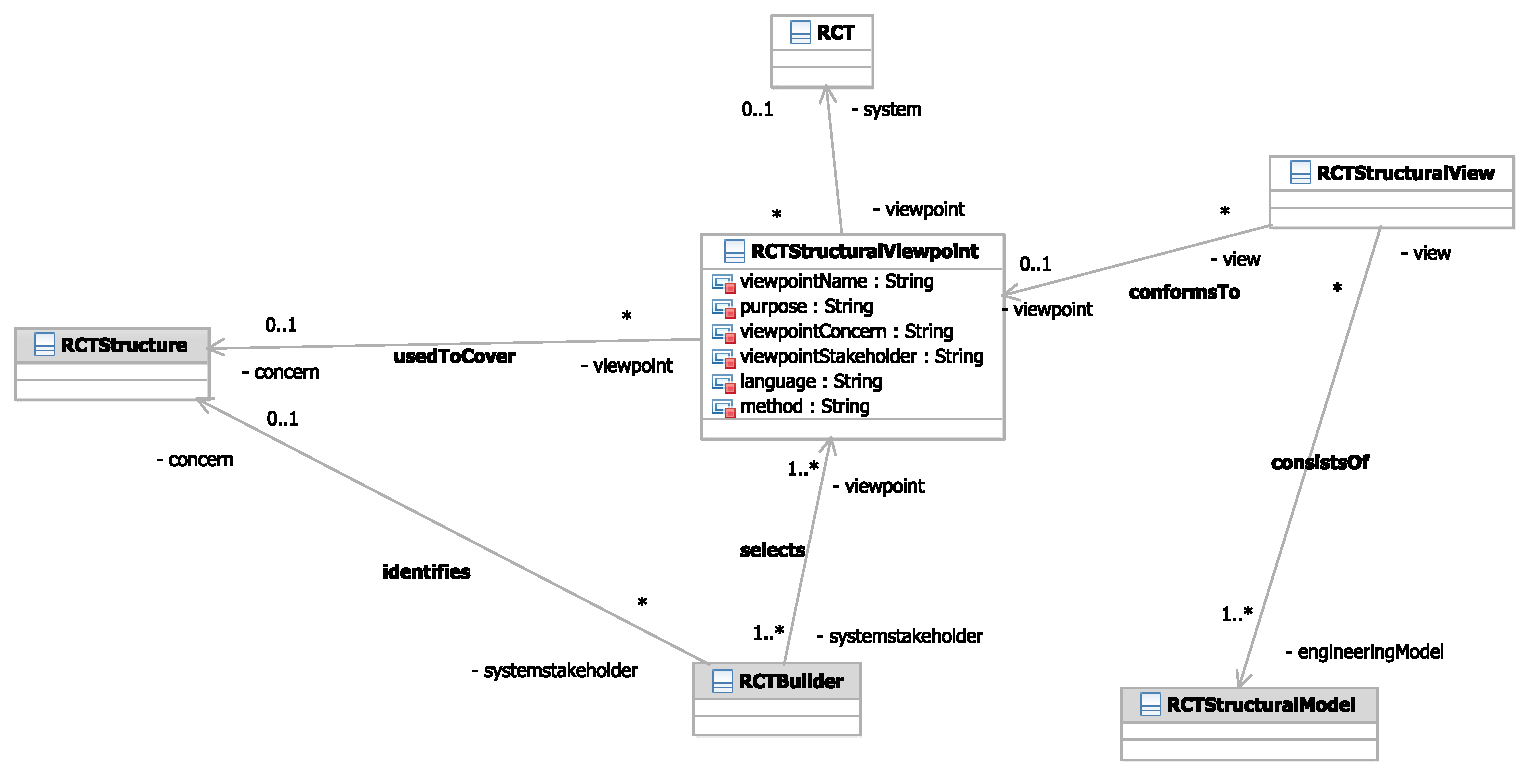
\includegraphics[width=0.95\textwidth]{RCT_RCTStructuralViewpointModel.pdf}}
\end{center}
\caption{RCT StructuralViewpoint Model}
\label{fig:RCTstructuralviewpointmodel}
\end{figure}

Additionally, the \emph{BehaviouralViewpoint} describes the autonomous system's behaviours, i.e., how the system operates under certain conditions. The RCTBehaviouralViewpointModel obtained (Fig. \ref{fig:RCTbehaviouralviewpointmodel}) instantiates the concepts and relationships in the Perspective and the ASysPerspective Packages. The different roles played for the concepts in the model are shown in each one of the relationships, which are given the same name as in the original package.\\


\begin{figure}[htbp]
\begin{center}
 {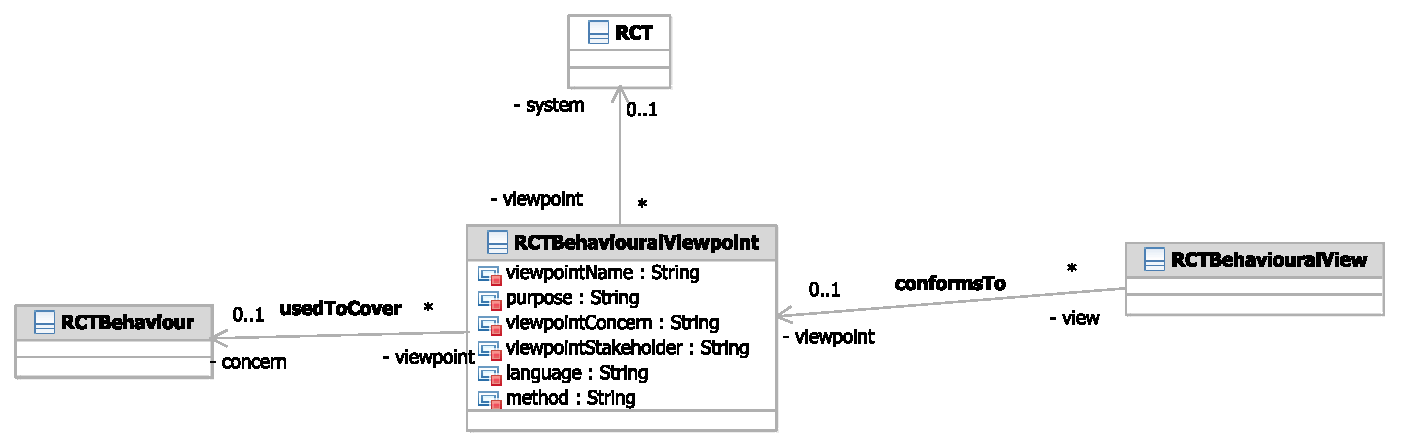
\includegraphics[width=0.95\textwidth]{RCT_RCTBehaviouralViewpointModel.pdf}}
\end{center}
\caption{RCT BehaviouralViewpoint Model}
\label{fig:RCTbehaviouralviewpointmodel}
\end{figure}

In turn, the \emph{FunctionalViewpoint} focus on the analysis of an autonomous system's functions, as desired or expected behaviours. The RCTStructuralViewpointModel (Fig. \ref{fig:RCTfunctionalviewpointmodel}) instantiates the  Perspective and the ASysPerspective Packages ontological elements, focusing on the functional aspects to consider for the RCT. In this model,  the RCTFunctionalView is a \emph{View} formalises as a RCTFunctionalModel, which is the \emph{EngineeringModel} consisting of different function related models, obtained as outputs of the FunctionalModelling subtask.\\

\begin{figure}[htbp]
\begin{center}
 {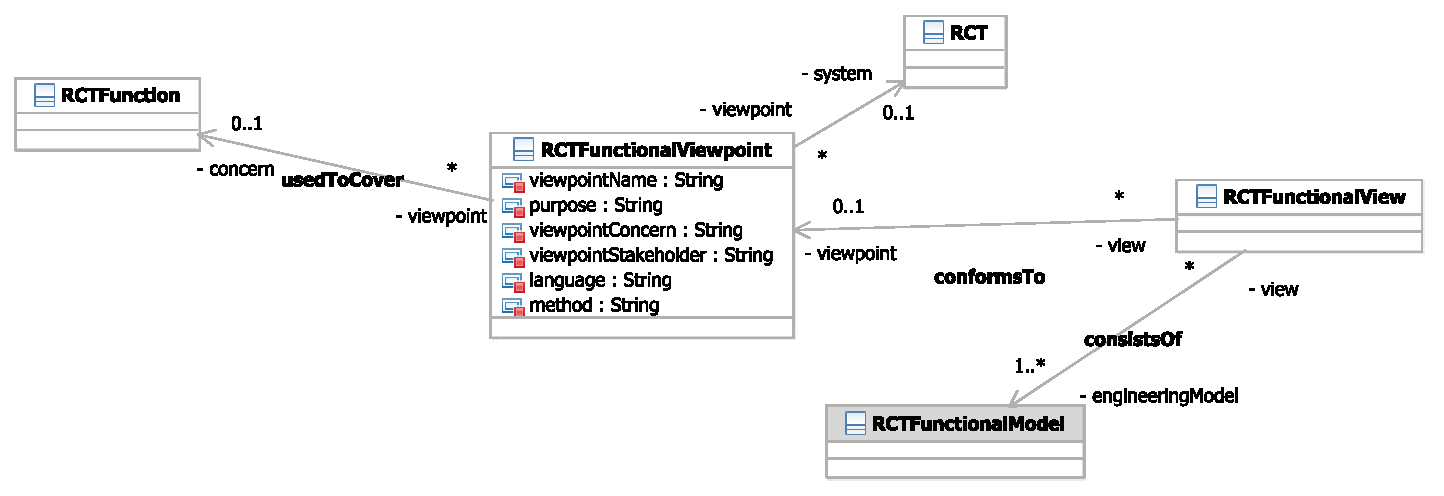
\includegraphics[width=0.95\textwidth]{RCT_RCTFunctionalViewpointModel.pdf}}
\end{center}
\caption{RCT FunctionalViewpoint Model}
\label{fig:RCTfunctionalviewpointmodel}
\end{figure}



During the RCT development, it will be necessary to address the \emph{PerformanceViewpoint}, to evaluate the performance requirements and benchmarking of the RCT once it is finally implemented. The PerformanceViewpoint addresses the performance aspects of the RCT. The Perspective and the ASysPerspective Package ontological elements were used to build up a PerformanceViewpointModel for the RCT (Fig. \ref{fig:RCTperformanceviewpointmodel}).\\

\begin{figure}[htbp]
\begin{center}
 {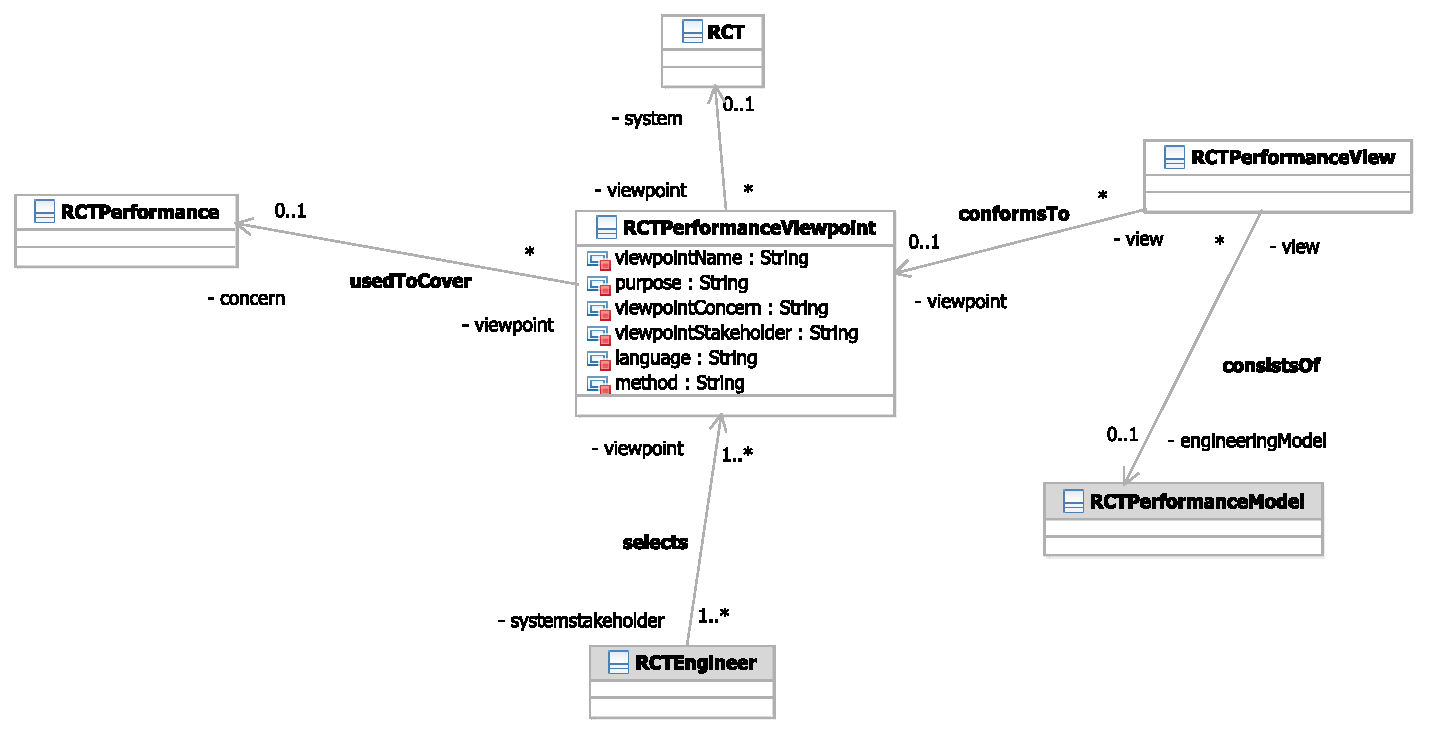
\includegraphics[width=0.95\textwidth]{RCT_RCTPerformanceViewpointModel.pdf}}
\end{center}
\caption{RCT PerformanceViewpoint Model}
\label{fig:RCTperformanceviewpointmodel}
\end{figure}


\section{RCT ASys Requirement Phase}

The purpose of this phase is to identify and elicit stakeholders' requirements for the RCT considering the RequirementViewpoint. The requirements are to be specified during this phase, by using traditional requirements engineering techniques.\\ 

\begin{itemize}
\item System UseCase Task

The first \emph{Task} during the \emph{ASys Requirement Phase} is to analyse the \emph{System UseCase}s, by instantiating the Requirement Package' ontological elements in the SystemEngineering Subontology. This \emph{Task} consists of the \emph{Subtask}s of \emph{UseCaseModelling} and \emph{UseCaseDetailing}, as defined in the ASys Engineering Subontology.\\

An \emph{UseCase} in OASys has been defined as a mean to capture a requirement of a system, as defined in the Perspective Package.To define the UseCase, the \emph{Subject} as system under consideration, and the different \emph{UseCaseActor}s as objects that interact with the system are also identified, among other aspects. As a result, a \emph{SystemUseCaseModel} is obtained, detailing the previous identified elements. The UML classes in the model are instantiation of the original OASys concepts, this fact being specified by the UML roles names in the shown associations. \\




When the \emph{Subject} under study is the Robot Control Testbed, an RCT \emph{UseCaseModel} shows the RCT's requirements by means of use cases. A system's requirements can be of different types (physical, functional, performance, interface, design) as defined in the Requirement Package.  An initial requirement analysis made by the RCT developers, identified the \emph{FunctionalRequirement}s for the RCT, where this concept has been defined as a ''requirement that specifies an operation or behaviour that a system must perform'' in OASys. Primary \emph{FunctionalRequirement}s for the RCT are to navigate, as well as to survive.\\

The navigation requirement is captured by means of the \emph{UseCase} Navigation, which \emph{include}s the secondary \emph{FunctionalRequirement}s of being able to explore the environment, identify elements in the environment, and to avoid obstacles. These requirements are captured in the \emph{Usecase}s of EnvironmentExploration, Identification and ObstacleAvoidance respectively (Fig. \ref{navigationusecasemodel}). In turn, the \emph{FunctionalRequirement} of surviving is captured in the Survival \emph{UseCase}, which \emph{include}s the SubsystemFailure and Recharge \emph{UseCase}s (Fig. \ref{survivalusecasemodel}).  \\

\begin{figure}[htbp]
\begin{center}
 {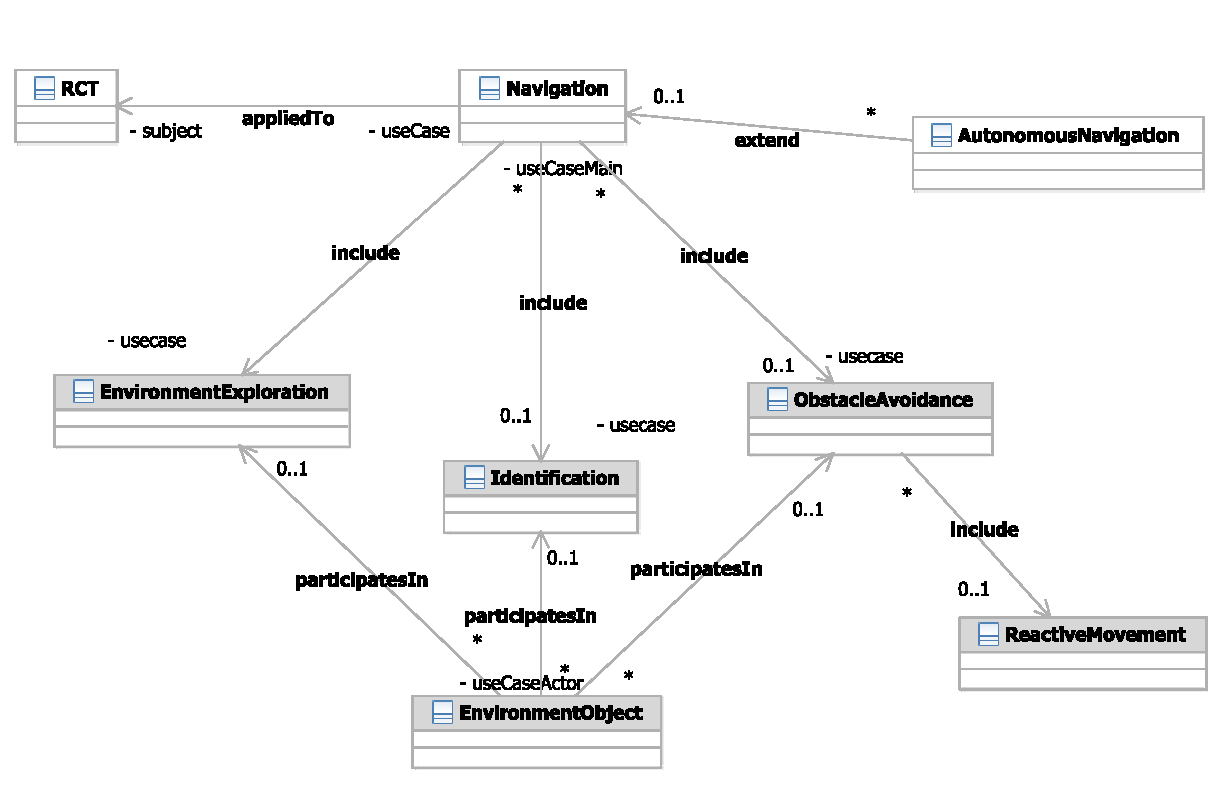
\includegraphics[width=0.95\textwidth]{RCT_RCTNavigationUseCaseModel.pdf}}
\end{center}
\caption{RCT Navigation UseCaseModel}
\label{navigationusecasemodel}
\end{figure}

\begin{figure}[htbp]
\begin{center}
 {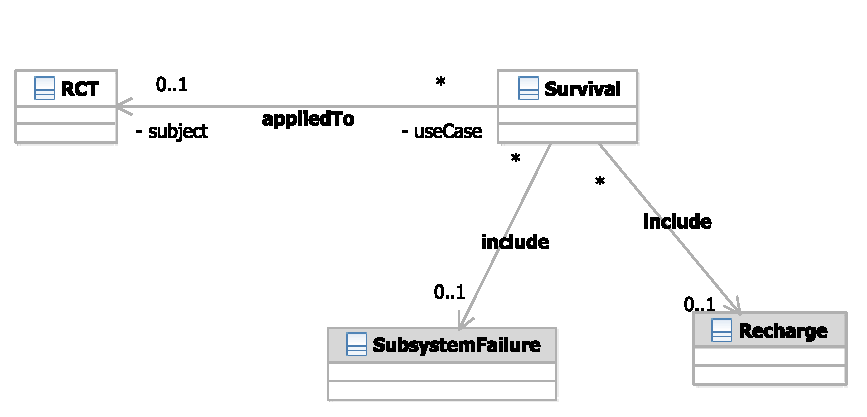
\includegraphics[width=0.85\textwidth]{RCT_RCTSurvivalUseCaseModel.pdf}}
\end{center}
\caption{RCT Survival UseCaseModel}
\label{survivalusecasemodel}
\end{figure}

It might be interesting to detail a particular \emph{UseCase} by paying attention to the \emph{Subsystem}s in the \emph{System}, to detail further \emph{Requirement}s. \emph{Subsystem}s identified in the RCT are the BasePlatform, the OnboardSystem, and the SupportingSystem. Focusing, for example, on the Navigation \emph{UseCase} previously defined, it is possible to identify additional \emph{Requirement}s for the \emph{Subsystem}s, in the form of a RCT Subsystem \emph{UseCaseModel} (Fig. \ref{rctnavigationsubsystemusecasemodel}).\\

\begin{figure}[htbp]
\begin{center}
 {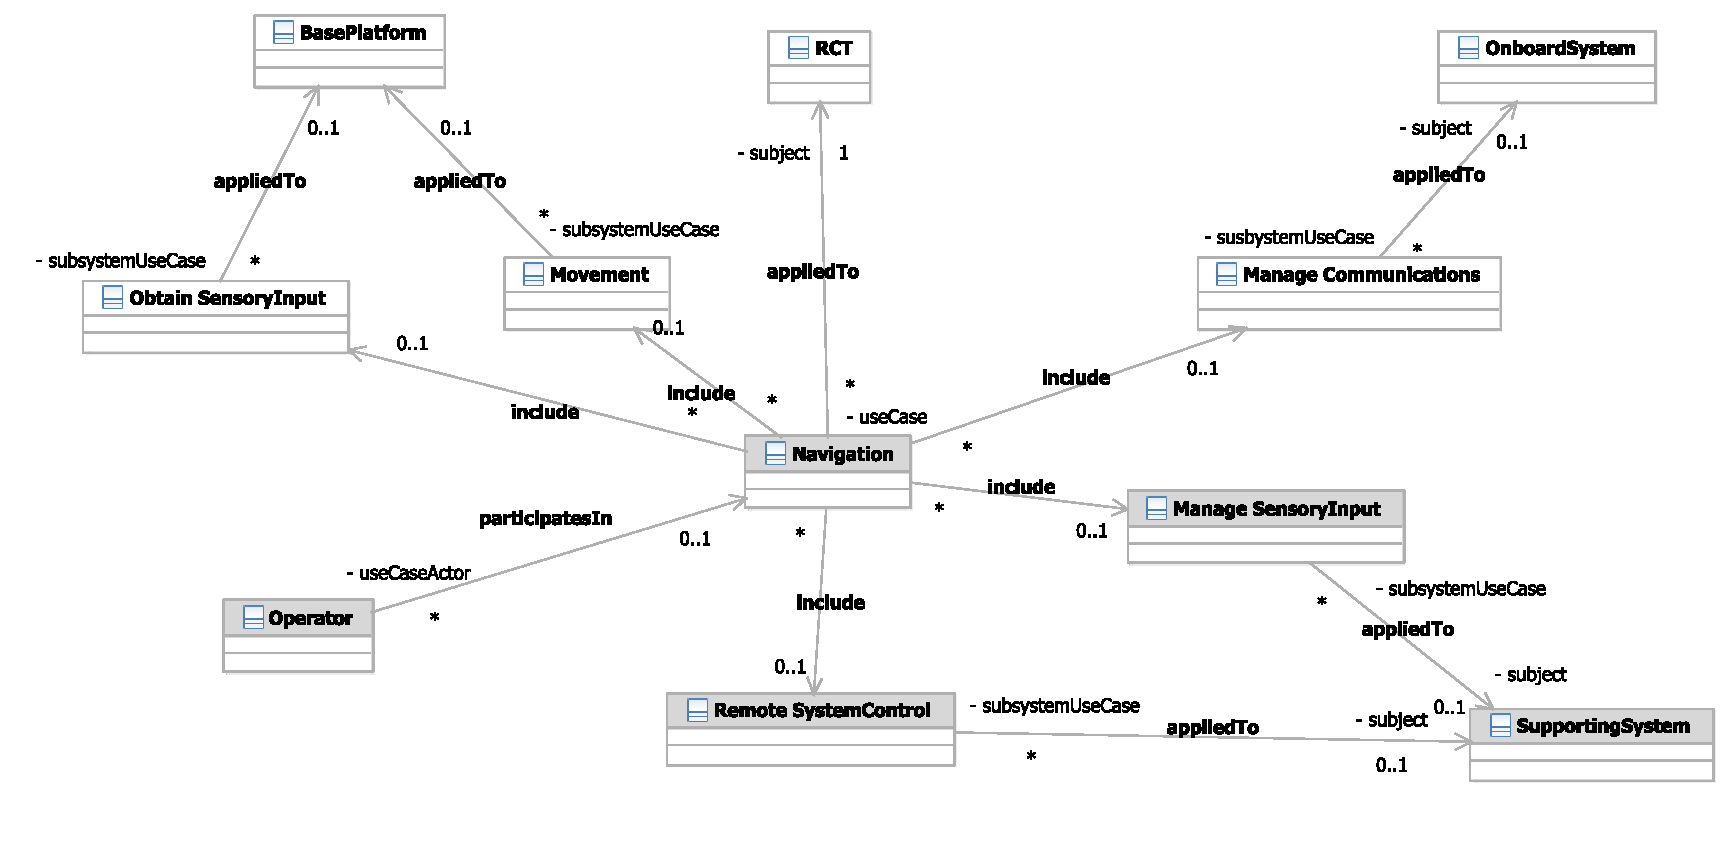
\includegraphics[width=0.95\textwidth]{RCT_SubsystemNavigationUseCaseModel.pdf}}
\end{center}
\caption{RCT Navigation UseCaseModel detailed for Subsystems}
\label{rctnavigationsubsystemusecasemodel}
\end{figure}

The \emph{UseCase Modelling Subtask} can also obtain a \emph{Subsystem UseCaseModel}, which gathers the \emph{Requirement} for a particular \emph{Subsystem}. In the case of the RCT, this subsystem usecasemodel was obtained for the BasePlatform (Fig. \ref{baseplatformusecasemodel}
 showing the instantiation of the original ontological elements) to detail the \emph{FunctionalRequirement} of movement; for the OnboardSystem to specify the \emph{FunctionalRequirement} of ManageCommunications (Fig. \ref{onboardusecasemodel}
); and for the SupportingSystem to clarify the Manage SensoryInput requirement (Fig. \ref{supportingsystemusecasemodel}).\\

\begin{figure}[htbp]
\begin{center}
 {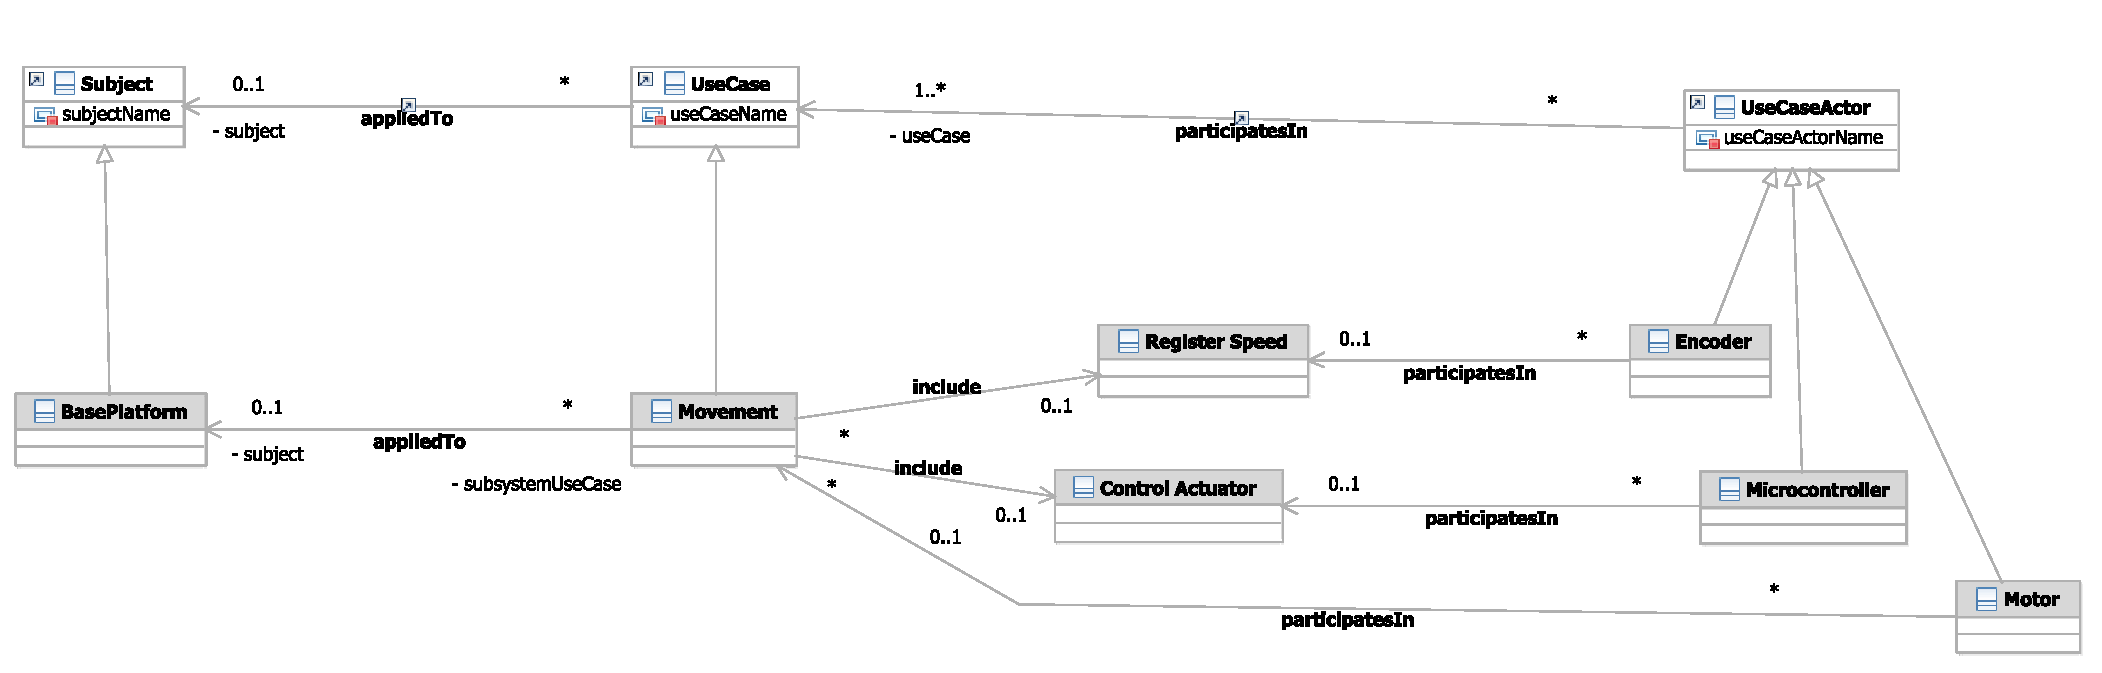
\includegraphics[width=0.85\textwidth]{RCT_BasePlatformMovementUseCaseModel.pdf}}
\end{center}
\caption{BasePlatform Subsystem UseCaseModel}
\label{baseplatformusecasemodel}
\end{figure}

\begin{figure}[htbp]
\begin{center}
 {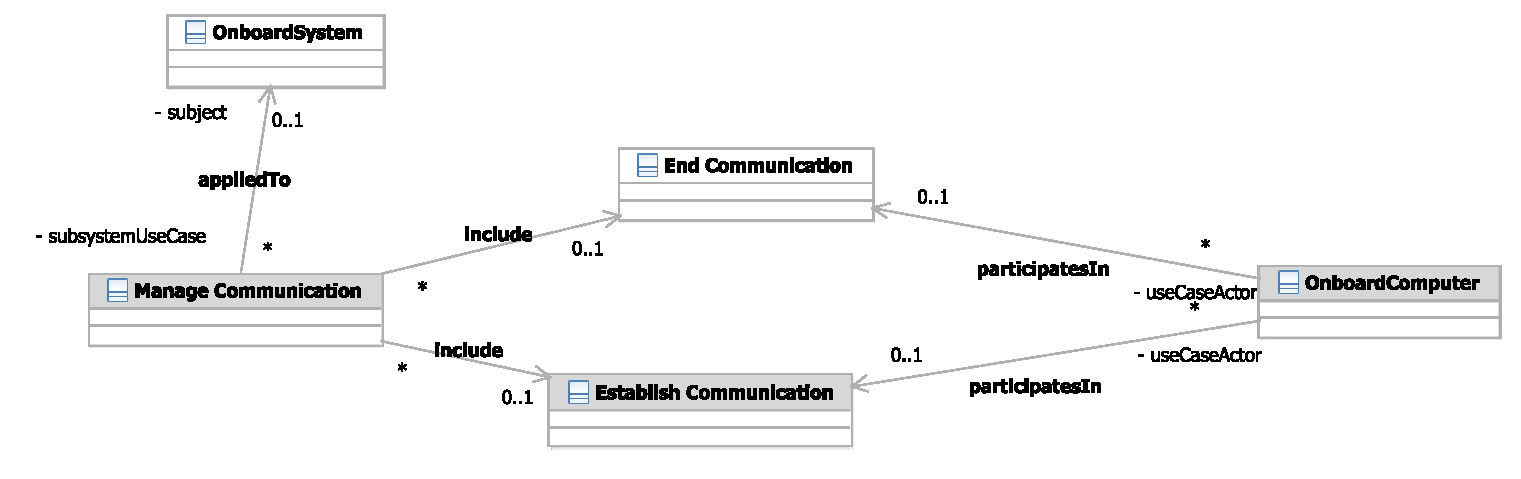
\includegraphics[width=0.85\textwidth]{RCT_OnBoardSystemManageCommunicationsUseCaseModel.pdf}}
\end{center}
\caption{OnboardSystem Subsystem UseCaseModel}
\label{onboardusecasemodel}
\end{figure}

\begin{figure}[htbp]
\begin{center}
 {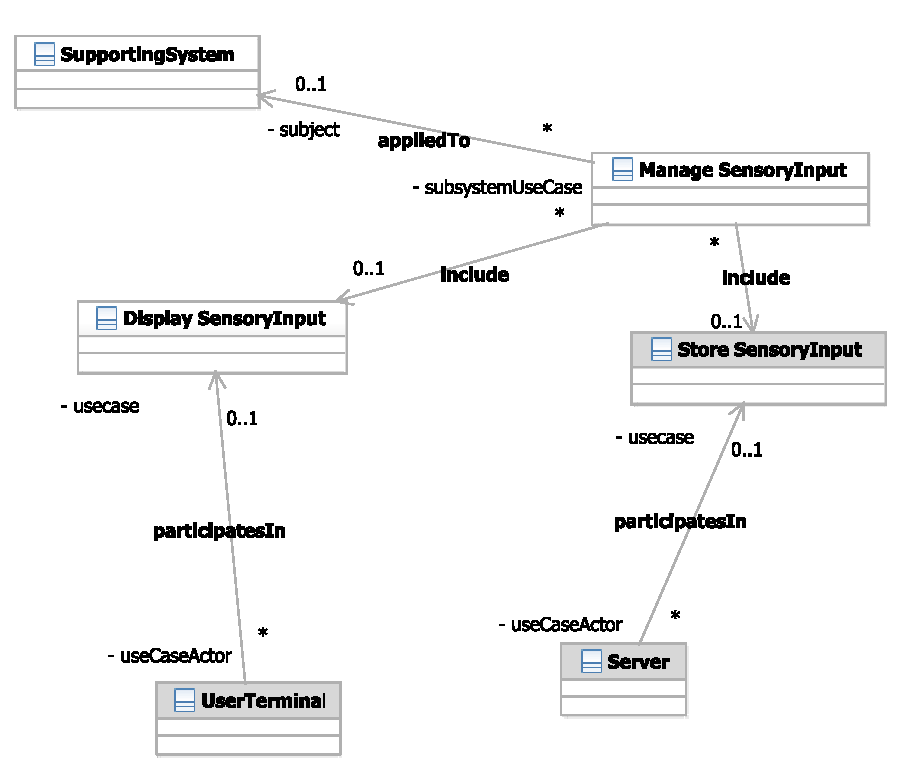
\includegraphics[width=0.75\textwidth]{RCT_SupportingSystemManageSensoryInputUseCaseModel.pdf}}
\end{center}
\caption{SupportingSystem Subsystem UseCaseModel}
\label{supportingsystemusecasemodel}
\end{figure}

The next \emph{Subtask} in the \emph{ASysRequirement Phase} is to detail each \emph{UseCaseModel} obtained during a \emph{UseCase Detailing Subtask}. This detail can be achieved by filling a pre--defined ASLab UseCase Pattern, with the relevant information in each field as required. This \emph{Subtask} was performed by the RCT developers, having as results different textual tables for the previous \emph{UseCase}s. For example, the detail for the Navigation requirement is shown in Fig. \ref{RCTnavigationdetailing}, and the Survival one in Fig. \ref{RCTsurvivaldetailing}.\\

\begin{figure}[htbp]
\begin{center}
 {\includegraphics[width=0.75\textwidth]{RCT-NavigationUseCaseDetailing.pdf}}
\end{center}
\caption{UseCase Detailing Subtask for the Navigation requirement}
\label{RCTnavigationdetailing}
\end{figure}

\begin{figure}[htbp]
\begin{center}
 {\includegraphics[width=0.75\textwidth]{RCT-SurvivalUseCaseDetailing.pdf}}
\end{center}
\caption{UseCase Detailing Subtask for the Survival requirement}
\label{RCTsurvivaldetailing}
\end{figure}


\item{Requirement Characterisation}

An additional \emph{Task} in this \emph{Phase} is to characterise the autonomous system's requirements, to obtain a \emph{RequirementCharacterisation}, as defined in the  ASys Engineering Process Package of the ASys Engineering Subontology. The taxonomies of concepts considered in the ASys Requirement Package can be described specifying a condition, a requirement criterion and a possible threshold. As a result, a \emph{Process Characterisation} and a \emph{System Characterisation} in the form of a textual description.\\ %look at MFESA book pp 374-375 to do this
\end{itemize}

\section{RCT ASys Analysis Phase}

As part of the ASys Analysis Phase consists of differents \emph{Tasks}, such as \emph{StructuralAnalysis}, \emph{BehaviouralAnalysis}, and \emph{FunctionalAnalysis}. The differents tasks have been carried out for the Robot Control Testbed, as described in following sections.\\

\begin{description}
\item \textbf{Structural Analysis}\\

The \emph{StructuralAnalysis Task} pays attention to the system under analysis from a \emph{StructuralViewpoint}, i.e., the analysis considering the system's structure in terms of subsystems and elements. As outcome of the task, a \emph{StructuralModel} for the RCT is obtained, consisting of \emph{StructureModel}s and\emph{Topology Model}s.\\

\begin{itemize}
\item System Modelling\\

The \emph{SystemModelling Subtask} carried out for the RCT has obtained the \emph{StructuralModel}, consisting of the \emph{StructureModel}s and the \emph{TopologyModel}s. For the RCT \emph{StructureModel}, the different subsystems part of it were determined according to the structural definition provided. Hence, three different kind of subsystem were identified: the platform, the onboard system attached to it, and the supporting system which are not physically part of the RCT but take part into its operation. The platform was further analysed to identify the subsystems or elements part of it. The different onboard systems were identified. Finally, the supporting systems were specified. The overall analysis result was formalised as a \emph{StructureModel} for the RCT (Fig. \ref{fig:RCTsystemmodel}). \\

\begin{figure}[htbp]
\begin{center}
 {\includegraphics[width=0.99\textwidth]{RCT_RCTStructureModel_1.pdf}}
\end{center}
\caption{RCT Structure Model}
\label{fig:RCTsystemmodel}
\end{figure}


The \emph{TopologyModel} allows representing the topological connections between a system's parts, by refining the Topology Package concepts. For the Robot Control Testbed, it was considered important to differentiate the topology from an informational and a physical aspects. The first one refers to the communication connections between parts, such as WiFi, Ethernet, etc. The latter, the physical connections among parts in a traditional way. Hence, two different topology models have been obtained for the RCT system: the RCT Informational Topology Model (Fig. \ref{fig:RCTinformationaltopologymodel}), and the RCT Physical Topology Model (Fig. \ref{fig:RCTphysicaltopologymodel}).\\

\begin{figure}[htbp]
\begin{center}
 {\includegraphics[width=0.75\textwidth]{RCT_RCTInformationalTopologyModel.pdf}}
\end{center}
\caption{RCT Topology Model: informational connections}
\label{fig:RCTinformationaltopologymodel}
\end{figure}

\begin{figure}[htbp]
\begin{center}
 {\includegraphics[width=0.99\textwidth]{RCT_RCTPhysicalTopologyModel.pdf}}
\end{center}
\caption{RCT Topology Model: physical connections}
\label{fig:RCTphysicaltopologymodel}
\end{figure}

Each one of the subsystems and elements identified in the \emph{StructureModel}, can be further detailed during a design phase to represent their characteristics and roles, by ontologically instantiating the concepts in the PhysicalDevice Package into a \emph{DeviceModel}. \\

%23 March 2010: I cannot longer use this, as I do not know how to make for the RSA does not show the values for the attributes
%An example is given in Fig. \ref{fig:RCTdevicemodel} for the Base Platform of the Robot Control Testbed. Additional attributes have been added as required, e.g. in the PowerSupply concept, to express specific design elements not included in the general ontological element. In a similar way, the computational devices and components can be detailed considering the Computational Device Package, to express software components, devices, and interfaces.\\

%\begin{figure}[htbp]
%\begin{center}
% {\includegraphics[width=0.90\textwidth]{RCT-DeviceModel.pdf}}
%\end{center}
%\caption{RCT Base Platform Device Model during design phase}
%\label{fig:RCTdevicemodel}
%\end{figure}


%TBD\item Knowledge Modelling

\end{itemize}
%TBD\item \textbf{Behavioural Analysis}

%TBD\item \textbf{Functional Analysis}

\end{description}




%===========================================================================
\chapter{Mission Specification}
%===========================================================================

%===========================================================================
\chapter{Higgs Webots Model}
%===========================================================================
 
\begin{figure}[htdp]
\begin{center}
 {\includegraphics[width=0.75\textwidth]{HiggsWebots.png}}
\end{center}
\caption{The Higgs virtualisation in Webots.}
\label{fig:HiggsWebots}
\end{figure}


%===========================================================================
\chapter{Model-based Synthesis}
%===========================================================================

This chapter will contains the description of the software synthesis process
from models.

%===========================================================================
\chapter{Higgs Self-Awareness}
%===========================================================================

This chapter will contains the description of the mechansisms for self-awareness
in Higgs.

\appendix
%===========================================================================
\chapter{CORBA Interface Definitions}
%===========================================================================


%===========================================================================
\chapter{XML Self-model}
%===========================================================================

The self-management system uses an XML model as the central repository of information on reflective knowledge. This is used by the self manager in the decision making concerning the functional operation of the robot.

What follows is the XML model concerning bandwidth-based reconfiguration of the robot perception system.

{\small
\begin{verbatim}
<?xml version="1.0" encoding="UTF-8"?>
<system xmlns="http://www.rcc.com/system"
    xmlns:xs="http://www.w3.org/2001/XMLSchema"
    xmlns:xsi="http://www.w3.org/2001/XMLSchema-instance"
    xsi:schemaLocation="http://www.rcc.com/system file:/C:/Users/raduadmin/Desktop/GPAC-0.13/metamodel/managedSystem.xsd">
    
    <name>BandwithControl</name>
    
    <resource>
        <ID>robot</ID>

		<!-- state parameter section -->
		
        <property>
            <ID>link_quality</ID>
            <propertyDataType>
                <xs:element name="link_quality" type="robotLink_quality" />
                <xs:simpleType name="robotLink_quality">
                    <xs:restriction base="xs:int"/>
                </xs:simpleType>
            </propertyDataType>
            <mutability>constant</mutability>
            <modifiability>read-only</modifiability>
            <subscribeability>false</subscribeability>
            <primaryKey>false</primaryKey>
        </property>
        <property>
            <ID>bit_rate</ID>
            <propertyDataType>
                <xs:element name="bit_rate" type="robotBit_rate" />
                <xs:simpleType name="robotBit_rate">
                    <xs:restriction base="xs:int"/>
                </xs:simpleType>
            </propertyDataType>
            <mutability>constant</mutability>
            <modifiability>read-only</modifiability>
            <subscribeability>false</subscribeability>
            <primaryKey>false</primaryKey>
        </property>
        <property>
            <ID>missed_beacons</ID>
            <propertyDataType>
                <xs:element name="missed_beacons" type="robotMissed_beacons" />
                <xs:simpleType name="robotMissed_beacons">
                    <xs:restriction base="xs:long"/>
                </xs:simpleType>
            </propertyDataType>
            <mutability>mutable</mutability>
            <modifiability>read-only</modifiability>
            <subscribeability>false</subscribeability>
            <primaryKey>false</primaryKey>
        </property>
        <property>
            <ID>video_fps</ID>
            <propertyDataType>
                <xs:element name="video_fps" type="robotVideo_fps" />
                <xs:simpleType name="robotVideo_fps">
                    <xs:restriction base="xs:double"/>
                </xs:simpleType>
            </propertyDataType>
            <mutability>constant</mutability>
            <modifiability>read-only</modifiability>
            <subscribeability>false</subscribeability>
            <primaryKey>false</primaryKey>
        </property>

		<!-- derived parameter section -->
		
		<property>
			<ID>bwidth_used</ID>
			<propertyDataType>
				<xs:element name="bwidth_used" type="robotBwidth_used" />
				<xs:simpleType name="robotBwidth_used">
					<xs:restriction base="xs:int"/>
				</xs:simpleType>
			</propertyDataType>
			<mutability>constant</mutability>
			<modifiability>read-only</modifiability>
			<subscribeability>false</subscribeability>
			<primaryKey>false</primaryKey>
		</property>


		<!-- configuration parameter section -->
		
		<property>
            <ID>video_rgb</ID>
            <propertyDataType>
                <xs:element name="video_rgb" type="robotVideo_rgb" />
                <xs:simpleType name="robotVideo_rgb">
                    <xs:restriction base="xs:int"/>
                </xs:simpleType>
            </propertyDataType>
            <mutability>constant</mutability>
            <modifiability>read-write</modifiability>
            <subscribeability>false</subscribeability>
            <primaryKey>false</primaryKey>
        </property>
        <property>
            <ID>video_width</ID>
            <propertyDataType>
                <xs:element name="video_width" type="robotVideo_width" />
                <xs:simpleType name="robotVideo_width">
                    <xs:restriction base="xs:int"/>
                </xs:simpleType>
            </propertyDataType>
            <mutability>constant</mutability>
            <modifiability>read-write</modifiability>
            <subscribeability>false</subscribeability>
            <primaryKey>false</primaryKey>
        </property>
        <property>
            <ID>video_trans</ID>
            <propertyDataType>
                <xs:element name="video_trans" type="robotVideo_trans" />
                <xs:simpleType name="robotVideo_trans">
                    <xs:restriction base="xs:int"/>
                </xs:simpleType>
            </propertyDataType>
            <mutability>constant</mutability>
            <modifiability>read-write</modifiability>
            <subscribeability>false</subscribeability>
            <primaryKey>false</primaryKey>
        </property>
        <property>
            <ID>laser_trans</ID>
            <propertyDataType>
                <xs:element name="laser_trans" type="robotLaser_trans" />
                <xs:simpleType name="robotLaser_trans">
                    <xs:restriction base="xs:int"/>
                </xs:simpleType>
            </propertyDataType>
            <mutability>constant</mutability>
            <modifiability>read-write</modifiability>
            <subscribeability>false</subscribeability>
            <primaryKey>false</primaryKey>
        </property>
        <property>
            <ID>sonars_trans</ID>
            <propertyDataType>
                <xs:element name="sonars_trans" type="robotSonars_trans" />
                <xs:simpleType name="robotSonars_trans">
                    <xs:restriction base="xs:int"/>
                </xs:simpleType>
            </propertyDataType>
            <mutability>constant</mutability>
            <modifiability>read-write</modifiability>
            <subscribeability>false</subscribeability>
            <primaryKey>false</primaryKey>
        </property>

		<!-- operational model section -->
		
		<property>
			<ID>operationalModel</ID>
			<propertyDataType>
				<xs:element name="operationalModel" type="robotOperationalModel"/>
				<xs:complexType name="robotOperationalModel">
					<xs:sequence>
						<xs:element name="modelElement" type="robotModelElement" maxOccurs="unbounded"/>
					</xs:sequence>
				</xs:complexType>
				<xs:complexType name="robotModelElement">
					<xs:sequence>
						<xs:element name="bwidth_used" type="robotBwidth_used" />
						<xs:element name="video_rgb" type="robotVideo_rgb" />
						<xs:element name="video_width" type="robotVideo_width" />
						<xs:element name="video_trans" type="robotVideo_trans" />
						<xs:element name="laser_trans" type="robotLaser_trans" />
						<xs:element name="sonars_trans" type="robotSonars_trans" />
						<xs:element name="video_fps" type="robotVideo_fps" />
					</xs:sequence>
				</xs:complexType>
			</propertyDataType>
			<mutability>constant</mutability>
			<modifiability>read-only</modifiability>
			<subscribeability>false</subscribeability>
			<primaryKey>false</primaryKey>
		</property>

	</resource>
</system>

\end{verbatim}
}

% ===============================================================================
% References
% ===============================================================================


\bibliography{bibliography}
\bibliographystyle{aslab}

\finalcover

\end{document}
